% Options for packages loaded elsewhere
\PassOptionsToPackage{unicode}{hyperref}
\PassOptionsToPackage{hyphens}{url}
\documentclass[
  12pt,
]{book}
\usepackage{xcolor}
\usepackage[margin=1in]{geometry}
\usepackage{amsmath,amssymb}
\setcounter{secnumdepth}{5}
\usepackage{iftex}
\ifPDFTeX
  \usepackage[T1]{fontenc}
  \usepackage[utf8]{inputenc}
  \usepackage{textcomp} % provide euro and other symbols
\else % if luatex or xetex
  \usepackage{unicode-math} % this also loads fontspec
  \defaultfontfeatures{Scale=MatchLowercase}
  \defaultfontfeatures[\rmfamily]{Ligatures=TeX,Scale=1}
\fi
\usepackage{lmodern}
\ifPDFTeX\else
  % xetex/luatex font selection
\fi
% Use upquote if available, for straight quotes in verbatim environments
\IfFileExists{upquote.sty}{\usepackage{upquote}}{}
\IfFileExists{microtype.sty}{% use microtype if available
  \usepackage[]{microtype}
  \UseMicrotypeSet[protrusion]{basicmath} % disable protrusion for tt fonts
}{}
\makeatletter
\@ifundefined{KOMAClassName}{% if non-KOMA class
  \IfFileExists{parskip.sty}{%
    \usepackage{parskip}
  }{% else
    \setlength{\parindent}{0pt}
    \setlength{\parskip}{6pt plus 2pt minus 1pt}}
}{% if KOMA class
  \KOMAoptions{parskip=half}}
\makeatother
\usepackage{color}
\usepackage{fancyvrb}
\newcommand{\VerbBar}{|}
\newcommand{\VERB}{\Verb[commandchars=\\\{\}]}
\DefineVerbatimEnvironment{Highlighting}{Verbatim}{commandchars=\\\{\}}
% Add ',fontsize=\small' for more characters per line
\newenvironment{Shaded}{}{}
\newcommand{\AlertTok}[1]{\textcolor[rgb]{1.00,0.00,0.00}{\textbf{#1}}}
\newcommand{\AnnotationTok}[1]{\textcolor[rgb]{0.38,0.63,0.69}{\textbf{\textit{#1}}}}
\newcommand{\AttributeTok}[1]{\textcolor[rgb]{0.49,0.56,0.16}{#1}}
\newcommand{\BaseNTok}[1]{\textcolor[rgb]{0.25,0.63,0.44}{#1}}
\newcommand{\BuiltInTok}[1]{\textcolor[rgb]{0.00,0.50,0.00}{#1}}
\newcommand{\CharTok}[1]{\textcolor[rgb]{0.25,0.44,0.63}{#1}}
\newcommand{\CommentTok}[1]{\textcolor[rgb]{0.38,0.63,0.69}{\textit{#1}}}
\newcommand{\CommentVarTok}[1]{\textcolor[rgb]{0.38,0.63,0.69}{\textbf{\textit{#1}}}}
\newcommand{\ConstantTok}[1]{\textcolor[rgb]{0.53,0.00,0.00}{#1}}
\newcommand{\ControlFlowTok}[1]{\textcolor[rgb]{0.00,0.44,0.13}{\textbf{#1}}}
\newcommand{\DataTypeTok}[1]{\textcolor[rgb]{0.56,0.13,0.00}{#1}}
\newcommand{\DecValTok}[1]{\textcolor[rgb]{0.25,0.63,0.44}{#1}}
\newcommand{\DocumentationTok}[1]{\textcolor[rgb]{0.73,0.13,0.13}{\textit{#1}}}
\newcommand{\ErrorTok}[1]{\textcolor[rgb]{1.00,0.00,0.00}{\textbf{#1}}}
\newcommand{\ExtensionTok}[1]{#1}
\newcommand{\FloatTok}[1]{\textcolor[rgb]{0.25,0.63,0.44}{#1}}
\newcommand{\FunctionTok}[1]{\textcolor[rgb]{0.02,0.16,0.49}{#1}}
\newcommand{\ImportTok}[1]{\textcolor[rgb]{0.00,0.50,0.00}{\textbf{#1}}}
\newcommand{\InformationTok}[1]{\textcolor[rgb]{0.38,0.63,0.69}{\textbf{\textit{#1}}}}
\newcommand{\KeywordTok}[1]{\textcolor[rgb]{0.00,0.44,0.13}{\textbf{#1}}}
\newcommand{\NormalTok}[1]{#1}
\newcommand{\OperatorTok}[1]{\textcolor[rgb]{0.40,0.40,0.40}{#1}}
\newcommand{\OtherTok}[1]{\textcolor[rgb]{0.00,0.44,0.13}{#1}}
\newcommand{\PreprocessorTok}[1]{\textcolor[rgb]{0.74,0.48,0.00}{#1}}
\newcommand{\RegionMarkerTok}[1]{#1}
\newcommand{\SpecialCharTok}[1]{\textcolor[rgb]{0.25,0.44,0.63}{#1}}
\newcommand{\SpecialStringTok}[1]{\textcolor[rgb]{0.73,0.40,0.53}{#1}}
\newcommand{\StringTok}[1]{\textcolor[rgb]{0.25,0.44,0.63}{#1}}
\newcommand{\VariableTok}[1]{\textcolor[rgb]{0.10,0.09,0.49}{#1}}
\newcommand{\VerbatimStringTok}[1]{\textcolor[rgb]{0.25,0.44,0.63}{#1}}
\newcommand{\WarningTok}[1]{\textcolor[rgb]{0.38,0.63,0.69}{\textbf{\textit{#1}}}}
\usepackage{graphicx}
\makeatletter
\newsavebox\pandoc@box
\newcommand*\pandocbounded[1]{% scales image to fit in text height/width
  \sbox\pandoc@box{#1}%
  \Gscale@div\@tempa{\textheight}{\dimexpr\ht\pandoc@box+\dp\pandoc@box\relax}%
  \Gscale@div\@tempb{\linewidth}{\wd\pandoc@box}%
  \ifdim\@tempb\p@<\@tempa\p@\let\@tempa\@tempb\fi% select the smaller of both
  \ifdim\@tempa\p@<\p@\scalebox{\@tempa}{\usebox\pandoc@box}%
  \else\usebox{\pandoc@box}%
  \fi%
}
% Set default figure placement to htbp
\def\fps@figure{htbp}
\makeatother
\setlength{\emergencystretch}{3em} % prevent overfull lines
\providecommand{\tightlist}{%
  \setlength{\itemsep}{0pt}\setlength{\parskip}{0pt}}
\usepackage[utf8]{inputenc} \usepackage[T1]{fontenc} \usepackage{textalpha} \usepackage{tikz} \usepackage{upquote} \usepackage{wrapfig} \usepackage{graphicx} \usepackage{amsmath} \usepackage{circuitikz} \usepackage{color}
\usepackage{bookmark}
\IfFileExists{xurl.sty}{\usepackage{xurl}}{} % add URL line breaks if available
\urlstyle{same}
% fallback for those not using the hyperref driver hyperxmp:
\makeatletter
\@ifundefined{xmpquote}{\newcommand{\xmpquote}[1]{#1}}{}
\makeatother
\hypersetup{
  pdftitle={The Nim programming language},
  pdfauthor={Victor Della-Vos; Proofreading -- Lecale, Marcus; Illustrations -- Priscila},
  hidelinks,
  pdfcreator={LaTeX via pandoc}}

\title{The Nim programming language}
\author{Victor Della-Vos \and Proofreading -- Lecale,
Marcus \and Illustrations -- Priscila}
\date{}

\begin{document}
\frontmatter
\maketitle

\mainmatter
\usetikzlibrary{backgrounds, positioning, %% Draw Y-chart
                     snakes, fit,       %% Draw Y-chart
                   3d,  arrows, automata, shapes.gates.logic.US,
                   shapes.gates.logic.IEC, calc, 
                    circuits.logic.US}

\mainmatter

\chapter{Hello, World!}\label{hello-world}

Since you are reading this tutorial, I assume that you want to learn the
Nim computer language. It is a long tradition in Computer Science to
start a tutorial concerning programming with a demo that shows how to
output messages to a terminal. However, you must learn many things
before actually being able to make such a demo work. Therefore, I
suggest that you call a geek who has majored in Computer Science to run
the applications presented in this first chapter, which will deal with
sending messages for printing on a terminal. I will use exercises
created by Kaushal Modi to get your attention, and entice you into Nim
programming. Here is the first program:

\begin{Shaded}
\begin{Highlighting}[]
\KeywordTok{import}\NormalTok{ os}\KeywordTok{,}\NormalTok{ std}\CommentTok{/}\NormalTok{terminal}

\DataTypeTok{styledEcho } \StringTok{"Hello, "}\KeywordTok{,}\NormalTok{ styleBright}\KeywordTok{,}\NormalTok{ fgCyan}\KeywordTok{,} \DataTypeTok{paramStr}\KeywordTok{(}\DecValTok{1}\KeywordTok{)}
\end{Highlighting}
\end{Shaded}

Let us assume that the geek, who you hired to coach you through this
demo, has discovered a way of writing the above program into the
\texttt{hi.nim} file. This time she uses SBEmacs. Open SBEmacs, press
\textbf{C-x C-f}, and type the path of \texttt{hi.nim} in your working
folder. Enter the following program:

\begin{Shaded}
\begin{Highlighting}[]
\KeywordTok{import}\NormalTok{ os}\KeywordTok{,}\NormalTok{ std}\CommentTok{/}\NormalTok{terminal}
\DataTypeTok{styledEcho} \StringTok{"Hi, "}\KeywordTok{,}\NormalTok{ styleItalic}\KeywordTok{,}\NormalTok{ fgBlue}\KeywordTok{,} \DataTypeTok{paramStr}\KeywordTok{(}\DecValTok{1}\KeywordTok{)}
\end{Highlighting}
\end{Shaded}

Press \textbf{SAVE} or \textbf{C-x C-s}. The program is visible in the
editor, so there is no need to use \texttt{cat} to check the file. Nim
mode colors the source and indents with two spaces when you press
\textbf{TAB}. If necessary, use \textbf{M-x load-mode}, enter
\textbf{nim}, and press Enter. The mode is distributed in the
repository's \texttt{sbemacs/nim-mode.lisp}; installation is explained
in \texttt{sbemacs/README.md}.

Finally, it is necessary to compile the program. This means that the
geek will convert the \texttt{hi.nim} source file into an executable
file, which the machine understands well enough in order to carry out
the instructions.

Choose \textbf{MORE}, then \textbf{Build}, or type \textbf{M-x
nim-build}. SBEmacs saves the source and calls the Nim compiler. The
lower window shows the compiler output. \textbf{C-x 1} closes this
window and returns to the source.

The final step is to execute the program to test whether it is
functioning correctly. Choose \textbf{MORE}, then \textbf{Run}, or type
\textbf{M-x nim-run}. At \textbf{Nim program arguments:} type
\texttt{Edward} and press Enter. This compiles and runs the current
file. Its output appears inside SBEmacs:

\begin{Shaded}
\begin{Highlighting}[]
\NormalTok{Hi, Edward}
\end{Highlighting}
\end{Shaded}

The shell output buffer displays plain text; it does not render the
terminal's blue italic styling. To obtain plain output you can also use
\texttt{echo\ "Hi,\ ",\ paramStr(1)}. No separate terminal window is
needed to edit, compile or run this example.

In chapter \ref{chap:tacit}, I will discuss knowledge. Then you will
learn that knowledge can be explicit, tacit and shared. To discover how
this can affect your study of the Nim programming language, let us see
what Socrates said about knowledge.

Calias had two sons. Of course, he spent a lot of money hiring teachers
for his sons. So, Socrates asked him: \emph{``Calias, if your sons were
colts or calves, we could find and engage a trainer for them who would
make them excel in their proper qualities, some horse breeder or farmer.
Now since they are men, whom do you have in mind to coach them? Who is
an expert in this kind of excellence, oratory and political debate? I
think you must have given thought to this since you have sons. Is there
such a person,''} Socrates asked, \emph{``or is there not?''}
\emph{``For sure there is,''} Calias said. \emph{``Who is he?''}
Socrates asked, \emph{``What is his name, where is he from? and what is
his fee?''} Calias replied: \emph{``The coach you are looking for, dear
Socrates, is Evenus, a citizen from Paras. His fee is five minas.''}

At the time of Socrates, the all important human activity was political
discussion, thus Evenus taught how to debate in assemblies and councils.
Nowadays, people are more interested in computer programming, since
these Weapons of Math Destruction, as Cathy O'Neil calls them, rule our
lives. However, let us make an analogy. Let us suppose that you have two
children, like Calias. If you wanted them to play the violin, instead of
programming, you will start out buying a violin primer, such as Suzuki's
Violin School, Volume 1, but you would not expect that your children
learn music just by reading a book. Therefore, you will hire a music
coach that will go to your house three times a week, in order to
supervise your children's progress. If the coach insists in explaining
only music theory, you will probably fire her, as you know one must
practice a lot to become a proficient musician.

You can use the same rules that apply to music for learning computer
programming. Then you need a book, a coach and a lot of practice, if you
want to learn how to write effective code. In consequence, it is a good
idea that you really hire a major in computer science to guide your
first steps in the computer world. The coach will explain the meaning of
such terminologies as compiler, library, terminal, files, source editors
and applications. Another thing that you can expect from the coach is
that she will perform many activities on the computer for you to observe
and repeat.

\chapter{State machines}\label{state-machines}

My private library has many books in Ancient Greek, Latin, German,
Esperanto, French, Japanese, Chinese, Guarany, Russian and other
languages that I don't speak. Even so, I read the first two pages of
these books, to know whether it was worthwhile to learn the language and
read until the end. War and Peace is written in French and Russian, thus
I read the French part of the first page and put the book back on the
shelf, where it remained over many years as a feast for cockroaches that
ate the glue on the cover.

Keeping with my bad reading habits, I read only the first page of
Wittgenstein's Tratactus Logico-Philosophicus, which has a title in
Latin, but is written in German. Here is the first line of the
Tratactus:

\begin{enumerate}
\def\labelenumi{\arabic{enumi}.}
\tightlist
\item
  Die Welt ist alles, was der Fall ist.

  \begin{itemize}
  \tightlist
  \item
    1.1. Die Welt ist die Gesamtheit der Tatsachen, nicht der Dinge.
  \end{itemize}
\end{enumerate}

On the first line, an English speaker can recognize a lot of words, for
instance, \emph{Welt} must mean \emph{World}, \emph{alles} can be
translated by \emph{all} and \emph{Fall} is \emph{fall}. There was that
Roman deity, Fortune, who decided the destiny of the World by throwing
dice. It seems that Wittgenstein is saying that the World is all that
the state of the Fortune's dice indicates that it is.

On the second line, Wittgenstein is saying that the World is the
totality of facts, not of things. Of course, things do exist, but the
World is something beyond a set of things. What is the entity, which is
beyond a mere collection of things? Let us read a little further to see
if the philosopher sheds light on the subject.

\begin{quote}
Was der Fall ist, die Tatsache, ist das Bestehen von Sachverhalten.
\end{quote}

David Pears translates the above line as

\begin{quote}
\emph{What is a case -- a fact -- is the existence of states of
affairs.}
\end{quote}

In Latin, the word \emph{STATUS} (Romans used to write only in uppercase
letters) means the temporary attributes of a person or thing. What is an
attribute? It is the position, station, place, posture, order,
arrangement, condition, characteristic, aspect, feature, quality or
trait that a thing can possess. An attribute has values, for instance,
the attribute \emph{color} can have values such as red, green, blue,
yellow, etc. The \emph{position} attribute can be given by the values of
the Cartesian coordinates of the object.

Computers are state machines, therefore they are good for modeling the
world and its evolution through change of states. Computers themselves
have registers, where they can store the values of the attributes that
the machine represents. Computer programs abstract the registers into
variables. Therefore, a program represents states by sets of values for
its variables. To understand this point, let us consider a concrete
problem.

\begin{Shaded}
\begin{Highlighting}[]
\CommentTok{\# File: zeller.nim}
\KeywordTok{import}\NormalTok{ os}\KeywordTok{,}\NormalTok{ strutils}

\KeywordTok{proc }\StringTok{roman\_order}\KeywordTok{(}\DataTypeTok{m} \KeywordTok{:} \DataTypeTok{int}\KeywordTok{):} \DataTypeTok{int}\CommentTok{=}
  \KeywordTok{let}\NormalTok{ wm}\CommentTok{=} \KeywordTok{(}\DecValTok{14} \CommentTok{{-}}\NormalTok{ m}\KeywordTok{)} \CommentTok{div} \DecValTok{12}
  \OtherTok{result}\CommentTok{=}\NormalTok{ m }\CommentTok{+}\NormalTok{ wm}\CommentTok{*}\DecValTok{12} \CommentTok{{-}} \DecValTok{2}

\KeywordTok{proc }\StringTok{zr}\KeywordTok{(}\NormalTok{y}\KeywordTok{:}\DataTypeTok{int}\KeywordTok{,}\NormalTok{ m}\KeywordTok{:}\DataTypeTok{int}\KeywordTok{,}\NormalTok{ day}\KeywordTok{:}\DataTypeTok{int}\KeywordTok{):} \DataTypeTok{int}\CommentTok{=}
  \KeywordTok{let}
\NormalTok{    roman\_month}\CommentTok{=} \DataTypeTok{roman\_order}\KeywordTok{(}\NormalTok{m}\KeywordTok{)}
\NormalTok{    roman\_year}\CommentTok{=}\NormalTok{ y }\CommentTok{{-}} \KeywordTok{(}\DecValTok{14} \CommentTok{{-}}\NormalTok{ m}\KeywordTok{)} \CommentTok{div} \DecValTok{12}
\NormalTok{    century}\CommentTok{=}\NormalTok{  roman\_year }\CommentTok{div} \DecValTok{100}
\NormalTok{    decade}\CommentTok{=}\NormalTok{ roman\_year }\CommentTok{mod} \DecValTok{100}
  \OtherTok{result}\CommentTok{=} \KeywordTok{(}\NormalTok{day }\CommentTok{+} \KeywordTok{(}\DecValTok{13}\CommentTok{*}\NormalTok{roman\_month }\CommentTok{{-}} \DecValTok{1}\KeywordTok{)} \CommentTok{div} \DecValTok{5} \CommentTok{+}
\NormalTok{                 decade }\CommentTok{+}\NormalTok{ decade }\CommentTok{div} \DecValTok{4} \CommentTok{+}
\NormalTok{                 century }\CommentTok{div} \DecValTok{4} \CommentTok{+}
\NormalTok{                 century }\CommentTok{*} \CommentTok{{-}}\DecValTok{2}\KeywordTok{)} \CommentTok{mod} \DecValTok{7}

\KeywordTok{proc }\StringTok{main}\CommentTok{ }\KeywordTok{()} \CommentTok{=}
  \KeywordTok{let}
\NormalTok{    year }\CommentTok{=} \DataTypeTok{paramStr}\KeywordTok{(}\DecValTok{1}\KeywordTok{).}\DataTypeTok{parseInt}
\NormalTok{    month }\CommentTok{=} \DataTypeTok{paramStr}\KeywordTok{(}\DecValTok{2}\KeywordTok{).}\DataTypeTok{parseInt}
\NormalTok{    day }\CommentTok{=} \DataTypeTok{paramStr}\KeywordTok{(}\DecValTok{3}\KeywordTok{).}\DataTypeTok{parseInt}
  \DataTypeTok{echo} \DataTypeTok{zr}\KeywordTok{(}\NormalTok{year}\KeywordTok{,}\NormalTok{ month}\KeywordTok{,}\NormalTok{ day}\KeywordTok{)}

\DataTypeTok{main}\KeywordTok{()}
\end{Highlighting}
\end{Shaded}

\begin{enumerate}
\def\labelenumi{(\arabic{enumi})}
\tightlist
\item
  Day of the week by Zeller's congruence
\end{enumerate}

You certainly know that the word \texttt{December} means the tenth
month; it comes from the Latin word for ten, as attested in words such
as:

\begin{itemize}
\tightlist
\item
  decimal -- base ten.
\item
  decimeter -- tenth part of a meter.
\item
  decimate -- the killing of every tenth Roman soldier that performed
  badly in battle.
\end{itemize}

October is named after the Latin numeral for \emph{eighth}. In fact, the
radical \emph{Oct-} can be translated as \emph{eight}, like in
\emph{octave}, \emph{octal}, and \emph{octagon}. One could continue with
this exercise, placing September in the seventh, and November in the
ninth position in the sequence of months. But everybody and his brother
know that December is the twelfth, and that October is the tenth month
of the year. Why did the Romans give misleading names to these months?

Rome was purportedly founded by Romulus, who designed a calendar. March
was the first month of the year in the Romulus calendar. In order to get
acquainted with programming and the accompanying concepts, let us follow
the Canadian programmer Nia Vardalos, while she explores the Nim
programming language and calendar calculations.

If Nia wants the order for a given month in this mythical calendar
created by Romulus, she must subtract 2 from the order in the Gregorian
calendar, which happens to be in current use in the Western World since
it was instituted by Pope Gregory XIII in 1582. After the subtraction,
September becomes the seventh month; October, the eight; November, the
ninth and December, therefore, the tenth month.

Farming and plunder were the main occupations of the Romans, and since
winter is not the ideal season for either of these activities, the
Romans did not care much for January and February. However, Sosigenes of
Alexandria, at the request of Cleopatra and Julius Cæsar, designed the
Julian calendar, where January and February, the two deep winter months,
appear in positions 1 and 2 respectively. Therefore, a need for a
formula that converts from the modern month numbering to the old
sequence has arisen. In listing 1, this is done by the following
algorithm:

\begin{Shaded}
\begin{Highlighting}[]

\KeywordTok{proc }\StringTok{roman\_order}\KeywordTok{(}\DataTypeTok{m} \KeywordTok{:} \DataTypeTok{int}\KeywordTok{):} \DataTypeTok{int}\CommentTok{=}
  \KeywordTok{let}\NormalTok{ wm}\CommentTok{=} \KeywordTok{(}\DecValTok{14} \CommentTok{{-}}\NormalTok{ m}\KeywordTok{)} \CommentTok{div} \DecValTok{12}
  \OtherTok{result}\CommentTok{=}\NormalTok{ m }\CommentTok{+}\NormalTok{ wm}\CommentTok{*}\DecValTok{12} \CommentTok{{-}} \DecValTok{2}
\end{Highlighting}
\end{Shaded}

In the above formula, the variable \texttt{wm} will pick the value 1 for
months 1 and 2, and 0 for months from 3 to 12. In fact, for months from
3 to 12, \texttt{(14-m)} produces a number less than 12, and
\texttt{(14-m)\ div\ 12} is equal to 0. Therefore, the state of the
program for all months from March through December is given by
\texttt{wm=0} and \texttt{result=m-2}. When the variable \texttt{wm=0},
the expression to calculate \texttt{result} is reduced from
\texttt{result=m+wm×12-2} to \texttt{result=m-2}. This means that March
will become the Roman month 1, and December will become the Roman month
10.

The variable \texttt{wm} models the state of the world for the winter
months. By the way, \texttt{wm} stands for \emph{winter months}. Since
January is month 1, and February is month 2 in the Gregorian calendar,
\texttt{wm} is equal to 1 for these two winter months. In the case of
January, the state is given by: \texttt{m=1}, \texttt{wm=1},
\texttt{result=11}. For February, the state becomes \texttt{m=2},
\texttt{wm=1}, \texttt{result=12}.

The program of the listing 1 calculates the day of the week through
Zeller's congruence. In the procedure \texttt{zr(y,\ m,\ day)}, the
let-statement binds values to the following state variables:
\texttt{roman\_month}, \texttt{roman\_year}, \texttt{century} and
\texttt{decade}. The listing 1 shows that a state variable avoids
recalculating values that appear more than once in a program. This is
the case of \texttt{roman\_year}, which appears four times in the
\texttt{zr(y,m,day)} procedure. Besides this, by identifying important
subexpressions with meaningful names, the program becomes clearer and
cleaner.

\section{Compile and run}\label{compile-and-run}

After compiling the program of listing 1, one can calculate the day of
the week as a number between 0 and 6, which correspond to Sunday,
Monday, Tuesday, Wednesday, Thursday, Friday and Saturday. Open
\texttt{zeller.nim} with \textbf{C-x C-f} in SBEmacs, and save the
program of listing 1. Choose \textbf{MORE → Run}, or \textbf{M-x
nim-run}. At \textbf{Nim program arguments:} enter \texttt{2016\ 8\ 31}.
The output window shows the result:

\begin{Shaded}
\begin{Highlighting}[]
\NormalTok{3}
\end{Highlighting}
\end{Shaded}

Use \textbf{C-x 1} to return to the source. Chapter 3 explains how to
submit the compiler command yourself through SBEmacs's shell.

This means that August 31 of 2016 fell on a Wednesday.

\section{Sequence of statement}\label{sequence-of-statement}

In linguistics, a statement is a declarative sentence that describes a
state or a state variable. In a program, one may need a sequence of
statements to determine all state variables. In the programming language
Nim, a sequence of statements is indicated by indentation, i.e., all
statements that start at the same column belong to the same sequence.

\section{Procedures}\label{procedures}

In computer programming, a procedure is a sequence of statements that
isolates and determines a state. In Nim, the procedure can cause change
of state by performing destructive assignment into variables introduced
by the key word \texttt{var}, but there is no way of changing the value
of variables introduced by the keyword \texttt{let}, such as the
variables that appear in listing 1.

\section{How to repeat a sequence of
statements}\label{how-to-repeat-a-sequence-of-statements}

During a programmer's life, he or she may need to repeat a sequence of
statements to generate a succession of steps that will approach an end
state or value. This repetition process is called iteration after the
Latin word for path.

Leonardo Bigollo Pisano, a.k.a. Fibonacci, was speculating on how fast
the reproduction of rabbits would be. His breeding of rabbits has the
interesting properties of mating at the age of one month, thus, at the
end of her second month, the female produces a new pair of rabbits, a
male and a female. Then she keeps producing two babies a month for one
year.

Fibonacci concluded that the number A\textsubscript{n} of adult pairs in
a given month is equal to the total number R\textsubscript{n-1} of
rabbits, both babies and adults, from the previous month. The clever
fellow also perceived that, since each adult pair produces two babies a
month, the number of baby pairs in a given month is the number of adult
pairs from the previous month, which is the total number of rabbits from
two months before. The total number of rabbit pairs, that is adults plus
babies, in any given month is the sum of the pairs from the previous two
months.

\begin{Shaded}
\begin{Highlighting}[]
\CommentTok{\# File: iterfib.nim}
\KeywordTok{import}\NormalTok{ os}\KeywordTok{,}\NormalTok{ strutils}

\KeywordTok{proc }\StringTok{fib}\KeywordTok{(}\NormalTok{n}\KeywordTok{:} \DataTypeTok{int}\KeywordTok{):} \DataTypeTok{int} \CommentTok{=}
  \KeywordTok{var} \KeywordTok{(}\NormalTok{r1}\KeywordTok{,}\NormalTok{ r2}\KeywordTok{)} \CommentTok{=} \KeywordTok{(}\DecValTok{2}\KeywordTok{,} \DecValTok{1}\KeywordTok{)}
  \DataTypeTok{for}\NormalTok{ i }\CommentTok{in} \DecValTok{2}\KeywordTok{..}\NormalTok{n}\KeywordTok{:}
    \KeywordTok{(}\NormalTok{r1}\KeywordTok{,}\NormalTok{ r2}\KeywordTok{)} \CommentTok{=} \KeywordTok{(}\NormalTok{r1}\CommentTok{+}\NormalTok{r2}\KeywordTok{,}\NormalTok{ r1}\KeywordTok{)}
  \OtherTok{result}\CommentTok{=}\NormalTok{ r1}

\DataTypeTok{echo} \DataTypeTok{fib}\KeywordTok{(}\DataTypeTok{paramStr}\KeywordTok{(}\DecValTok{1}\KeywordTok{).}\DataTypeTok{parseInt}\KeywordTok{)}
\end{Highlighting}
\end{Shaded}

In the above program, the iteration is controlled by the for-loop, that
repeats a change of state over generations from 2 through \texttt{n} of
rabbits. Here is how the program is compiled and executed:

Open \texttt{iterfib.nim} in SBEmacs, save it, and use \textbf{M-x
nim-run}. Enter \texttt{5} at the arguments prompt. The output is:

\begin{Shaded}
\begin{Highlighting}[]
\NormalTok{13}
\end{Highlighting}
\end{Shaded}

Use \textbf{C-x 1} to return to the source. Repeat with \texttt{12} to
obtain \texttt{377}, the number of pairs at the end of Fibonacci's year.

\section{Recursion}\label{recursion}

Another way to discover the number of pairs in the previous generation
is to sum the number of pairs from three generations ago to the number
of pairs from two generations ago. This reasoning does nothing more than
apply the rule of finding the total number of pairs in the present
generation over the previous generation. Here is a program that uses
this idea:

\begin{Shaded}
\begin{Highlighting}[]
\CommentTok{\#› nim c {-}{-}nimcache:xx {-}o:recfib.x {-}d:danger {-}{-}hints:off recfib.nim}
\KeywordTok{import}\NormalTok{ os}\KeywordTok{,}\NormalTok{ strutils}
\KeywordTok{proc }\StringTok{fib}\KeywordTok{(}\NormalTok{n}\KeywordTok{:} \DataTypeTok{int}\KeywordTok{):} \DataTypeTok{int} \CommentTok{=}
  \DataTypeTok{if}\NormalTok{ n}\CommentTok{\textless{}}\DecValTok{2}\KeywordTok{:} \OtherTok{result}\CommentTok{=}\NormalTok{ n}\CommentTok{+}\DecValTok{1}
  \DataTypeTok{elif}\NormalTok{ n}\CommentTok{\textless{}}\DecValTok{3}\KeywordTok{:} \OtherTok{result}\CommentTok{=} \DataTypeTok{fib}\KeywordTok{(}\NormalTok{n}\CommentTok{{-}}\DecValTok{1}\KeywordTok{)}\CommentTok{+}\DataTypeTok{fib}\KeywordTok{(}\NormalTok{n}\CommentTok{{-}}\DecValTok{2}\KeywordTok{)}
  \DataTypeTok{else}\KeywordTok{:} \OtherTok{result}\CommentTok{=} \DataTypeTok{fib}\KeywordTok{(}\NormalTok{n}\CommentTok{{-}}\DecValTok{3}\KeywordTok{)}\CommentTok{+}\DataTypeTok{fib}\KeywordTok{(}\NormalTok{n}\CommentTok{{-}}\DecValTok{2}\KeywordTok{)}\CommentTok{+}\DataTypeTok{fib}\KeywordTok{(}\NormalTok{n}\CommentTok{{-}}\DecValTok{2}\KeywordTok{)}

\DataTypeTok{echo} \DataTypeTok{fib}\KeywordTok{(}\DataTypeTok{paramStr}\KeywordTok{(}\DecValTok{1}\KeywordTok{).}\DataTypeTok{parseInt}\KeywordTok{)}
\end{Highlighting}
\end{Shaded}

\begin{enumerate}
\def\labelenumi{(\arabic{enumi})}
\setcounter{enumi}{1}
\tightlist
\item
  Recursive Fibonacci function
\end{enumerate}

Open \texttt{recfib.nim}, save the listing, and run \textbf{M-x nim-run}
with argument \texttt{5}. SBEmacs displays \texttt{13}. Repeat with
\texttt{12} to obtain \texttt{377}. You can visit the procedure with
\textbf{M-x nim-next-definition} and return to the previous one with
\textbf{M-x nim-previous-definition}.

The program of listing 2 has many novelties. The first one is the
conditional execution of a sequence of statements. For instance,
\texttt{result=n+1} sets \texttt{result} to \texttt{n+1}, but only if
the condition \texttt{n\textless{}2} is met. On the same token,
\texttt{result=fib(n-1)+fib(n-2)} sets \texttt{result} to
\texttt{fib(n-1)+fib(n-2)}, if \texttt{n\textless{}3}.

However, the strangest feature of listing 2, is the use of the
\texttt{fib} function in the definition of \texttt{fib}. In other words,
the definition of \texttt{fib} calls itself. When such a thing happens,
computer scientists say that the definition is recursive.

Typically a recursive definition has two kinds of conditions, which in
Nim are introduced by the if-statement:

\begin{itemize}
\tightlist
\item
  Trivial conditions, which can be resolved using primitive operations.
\item
  General conditions, which can be broken down into simpler cases.
\end{itemize}

In listing 2, the trivial condition is --

\begin{itemize}
\tightlist
\item
  \texttt{if\ n\textless{}2:\ result=n+1}
\end{itemize}

The general conditions are introduced by the \texttt{elif} and
\texttt{else} clauses for rewriting the expression \texttt{fib(n)} into
one of the following expressions:

\begin{Shaded}
\begin{Highlighting}[]
\DataTypeTok{elif}\NormalTok{ n}\CommentTok{\textless{}}\DecValTok{3}\KeywordTok{:} \OtherTok{result}\CommentTok{=} \DataTypeTok{fib}\KeywordTok{(}\NormalTok{n}\CommentTok{{-}}\DecValTok{1}\KeywordTok{)}\CommentTok{+}\DataTypeTok{fib}\KeywordTok{(}\NormalTok{n}\CommentTok{{-}}\DecValTok{2}\KeywordTok{)}
\DataTypeTok{else}\KeywordTok{:} \OtherTok{result}\CommentTok{=} \DataTypeTok{fib}\KeywordTok{(}\NormalTok{n}\CommentTok{{-}}\DecValTok{3}\KeywordTok{)}\CommentTok{+}\DataTypeTok{fib}\KeywordTok{(}\NormalTok{n}\CommentTok{{-}}\DecValTok{2}\KeywordTok{)}\CommentTok{+}\DataTypeTok{fib}\KeywordTok{(}\NormalTok{n}\CommentTok{{-}}\DecValTok{2}\KeywordTok{)}
\end{Highlighting}
\end{Shaded}

Where each occurrence of a call to \texttt{fib} is closer to the trivial
case than \texttt{fib(n)}, which was the original call.

The mathematician Peano invented a very interesting axiomatic theory for
natural numbers, that can be summarized thus:

\begin{enumerate}
\def\labelenumi{\arabic{enumi}.}
\tightlist
\item
  Zero is a natural number.
\item
  Every natural number has a successor: The successor of 0 is 1, the
  successor of 1 is 2, the successor of 2 is 3, and so on.
\item
  If a property is true for zero and, after assuming that it is true for
  n, you prove that it is true for n+1, then it is true for any natural
  number.
\end{enumerate}

Did you get the idea? For this very idea can be applied to many other
situations, even in programming a computer.

Luciano Lima and Roger Alan think that it is very important to reproduce
Peano's theory in the Latin original. However, I decided against meeting
their demands for many reasons. In his book, Arithmetices Principia,
Peano adopted a notation that is beyond the reach of most readers.
Besides this, the 1889 edition by the Fratres Bocca has many typos that
I need to fix before considering it for inclusion in this book.

Sergio Teixeira and Stephanie Bourdieu said that my implementation of
the Fibonacci procedure was not faithful to the 1228 edition of the
Liber Abaci. I changed the algorithms as recommended by them, and also
reproduced the fable of the 377 rabbits that appear in chapter 12 of
Fibonacci's book.

Readers who do not know Latin, or are not interested in Fibonacci's
original work, can skip the rest of this chapter without any loss of
important information.

\subsubsection*{Liber Abaci -- Chapter XII: The Fable of the
Rabbits}\label{LiberAbaci}
\addcontentsline{toc}{subsubsection}{Liber Abaci -- Chapter XII: The
Fable of the Rabbits}

A certain man keeps one pair of rabbits in an enclosed place. This man
wishes to know how many rabbits will be generated by the original pair
in a period of one year. It is the nature of this breed of rabbits in a
single month to bear another pair, and in the second month those born to
bear also.

Since the individuals of the first pair of rabbits are adults, in the
first month, they will bear a pair of kittens, therefore the number of
animals will double; so, there will be two pairs in one month. One of
these, namely the first, bears in the second month, and thus there are
in the second month 3 pairs; of these in one month two are pregnant, and
in the third month 2 pairs of rabbits are born, and thus there are 5
pairs in the month; in this month 3 pairs are pregnant, and in the
fourth month there are 8 pairs, of which 5 pairs bear another 5 pairs;
these are added to the 8 pairs making 13 pairs in the fifth month; these
5 pairs that are born in this month do not mate in this month, but
another 8 pairs are pregnant, and thus there are in the sixth month 21
pairs; to these are added the 13 pairs that are born in the seventh
month; there will be 34 pairs in this month; to this are added the 21
pairs that are born in the eighth month; there will be 55 pairs in this
month; to these are added the 34 pairs that are born in the ninth month;
there will be 89 pairs in this month; to these are added again the 55
pairs that are born in the tenth month; there will be 144 pairs in this
month; to these are added again the 89 pairs that are born in the
eleventh month; there will be 233 pairs in this month.

To these are still added the 144 pairs that are born in the last month;
there will be 377 pairs, and this many pairs are produced from the
aforementioned pair of rabbits in the enclosed place at the end of the
one year.

You can indeed see in the margin how we operated, namely that we added
the first number to the second, namely the 1 to the 2, and the second to
the third, and the third to the fourth, and the fourth to the fifth, and
thus one after another until we added the tenth to the eleventh, namely
the 144 to the 233, and we had the total sum of rabbits, i.e.~377. Thus,
you can systematically find the number of rabbits for an indeterminate
number of months.

\subsubsection*{Liber Abaci -- Capitulum XII: Fabula
Cuniculorim}\label{Liber}
\addcontentsline{toc}{subsubsection}{Liber Abaci -- Capitulum XII:
Fabula Cuniculorim}

Quot paria coniculorum in uno anno ex uno pario germinentur?

Quidam posuit unum par cuniculorum in quodam loco, qui erat undique
pariete circundatus, ut sciret, quot ex eo paria germinarentur in uno
anno: cum natura eorum sit per singulum mensem aliud par germinare; et
in secundo mense ab eorum nativitate germinant.

Quia suprascriptum par in primo mense germinat, duplicabis ipsum, erunt
paria duo in uno mense. Ex quibus unum, silicet primum, in secundo mense
geminat; et sic sunt in secundo mense paria 3; ex quibus in uno mense
duo pregnantur; et geminantur in tercio mense paria 2 coniculorum; et
sic sunt paria 5 in ipso mense; ex quibus in ipso pregnantur paria 3; et
sunt in quarto mense paria 8; ex quibus paria 5 geminant alia paria 5:
quibus additis cum pariis 8, faciunt paria 13 in quinto mense; ex quibus
paria 5, que geminata fuerunt in ipso mense, non concipiunt in ipso
mense, sed alia 8 paria pregnantur; et sic sunt in sexto mense paria 21;
cum quibus additis parijs 13, que geminantur in septimo, erunt in ipso
paria 34, cum quibus additis parijs 21, que geminantur in octavo mense,
erunt in ipso paria 55; cum quibus additis parijs 34, que geminantur in
nono mense, erunt in ipso paria 89; cum quibus additis rursum parijs 55,
que geminantur in decimo, erunt in ipso paria 144; cum quibus additis
rursum parijs 89, que geminantur in undecimo mense, erunt in ipso paria
233. Cum quibus etiam additis parijs 144, que geminantur in ultimo
mense, erunt paria 377, et tot paria peperit suprascriptum par in
prefato loco in capite unius anni. Potes enim videre in hac margine,
qualiter hoc operati fuimus, scilicet quod iunximus primum numerum cum
secundo, videlicet 1 cum 2; et secundum cum tercio; et tercium cum
quarto; et quartum cum quinto, et sic deinceps, donec iunximus decimum
cum undecimo, videlicet 144 cum 233; et habuimus suprascriptorum
cuniculorum summam, videlicet 377; et sic posses facere per ordinem de
infinitis numeris mensibus.

The farmer of Fibonacci's fable starts with a pair of addult rabbits.
Therefore, at the end of month 1, there were two pairs of rabbits. In
the instant zero of the experiment there was only the original pair.
Therefore, in listing 2, one has the following clause for
\texttt{n\textless{}2}:

\begin{Shaded}
\begin{Highlighting}[]
  \DataTypeTok{if}\NormalTok{ n}\CommentTok{\textless{}}\DecValTok{2}\KeywordTok{:} \OtherTok{result}\CommentTok{=}\NormalTok{ n}\CommentTok{+}\DecValTok{1}
\end{Highlighting}
\end{Shaded}

Since in the most general clause Stephanie needed three generations of
rabbits, she added a clause for the second month, to wit:

\begin{Shaded}
\begin{Highlighting}[]
  \DataTypeTok{elif}\NormalTok{ n}\CommentTok{\textless{}}\DecValTok{3}\KeywordTok{:} \OtherTok{result}\CommentTok{=} \DataTypeTok{fib}\KeywordTok{(}\NormalTok{n}\CommentTok{{-}}\DecValTok{1}\KeywordTok{)}\CommentTok{+}\DataTypeTok{fib}\KeywordTok{(}\NormalTok{n}\CommentTok{{-}}\DecValTok{2}\KeywordTok{)}
\end{Highlighting}
\end{Shaded}

From the second month onward Stephanie can use the most general clause:

\begin{Shaded}
\begin{Highlighting}[]
  \DataTypeTok{else}\KeywordTok{:} \OtherTok{result}\CommentTok{=} \DataTypeTok{fib}\KeywordTok{(}\NormalTok{n}\CommentTok{{-}}\DecValTok{3}\KeywordTok{)}\CommentTok{+}\DataTypeTok{fib}\KeywordTok{(}\NormalTok{n}\CommentTok{{-}}\DecValTok{2}\KeywordTok{)}\CommentTok{+}\DataTypeTok{fib}\KeywordTok{(}\NormalTok{n}\CommentTok{{-}}\DecValTok{2}\KeywordTok{)}
\end{Highlighting}
\end{Shaded}

In general, recursive calculation of Fibonacci's function is very
inefficient, and is often used in benchmarks. However, good compilers
succeed to optimize the recursion away, therefore the algorithm given by
listing 2 is very fast.

\chapter{Shell}\label{shell}

Nia, a young Greek woman, has an account on a well-known social network.
She visits her friends' postings on a daily basis, and when she finds an
interesting picture or video, she presses the \emph{Like}-button.
However, when she needs to discuss her upcoming holidays on the Saba
Island with her Argentinian boyfriend, she uses the live chat box. After
all, hitting buttons and icons offers only a very limited interaction
tool, and does not produce a highly detailed level of information that
is possible in a chat box.

Using a chat service needs to be very easy and fun, otherwise teenagers
would be doing something else. I am telling you this, because there are
two ways of commanding the operating system (OS) that the computer uses
to control mouse, keyboard, mass storage devices, etc. The first is
called Graphical User Interface (GUI) and consists of moving a mouse and
clicking over a menu option or an icon, such as the \texttt{Like}
button. As previously mentioned, a GUI often does not generate adequate
information for making a request to the OS. In addition, finding the
right object to press can become difficult in a labyrinth of menu
options.

The other method of interacting with the computer is known as Shell, and
is similar to a chat service. On a Shell interface, Nia issues
instructions that the operating system (OS) answers by fulfilling the
assigned tasks. The language that Nia uses to chat with the OS is called
\emph{bash}. Another option is \emph{zsh}, but it is so similar to
\emph{bash} that it does not require a separate tutorial. Languages such
as \emph{bash} and \emph{zsh} have commands to go through folders,
browser files, create new directories, copy objects from one place to
the other, configure the machine, install applications, change the
permissions of a file, etc. When accessing the OS through a text-based
terminal, a shell language is the main way of executing programs and
doing work on a computer.

SBEmacs provides a shell command window. From the file you are editing,
press \textbf{M-!} (Esc followed by the exclamation mark) or
\texttt{C-x\ @}. Write a command in the lower window, then press
\textbf{SEND} or \textbf{C-c s}. The result appears in
\texttt{*output*}. \textbf{C-x 1} closes the shell window and returns to
the file; \textbf{M-!} opens a fresh command window.

\section*{The prompt}\label{The}
\addcontentsline{toc}{section}{The prompt}

Files are stored in folders. Typically, the prompt shows the folder
where the user is currently working. The main duty of the operating
system is to maintain the content of the mass storage devices in a tree
structure of files and folders. Folders are also called
\emph{directories}, and like physical folders or cabinets, they organize
files. A folder can be put inside another folder. Your \texttt{HOME} is
your personal directory.

In SBEmacs, the shell command starts in the directory of the file from
which you pressed \textbf{M-!}. There is no persistent shell prompt.
Each \textbf{SEND} starts a new shell process: a \texttt{cd} command
does not change the directory of the next submission. Put \texttt{cd}
and the command that depends on it in the same submission:

\begin{Shaded}
\begin{Highlighting}[]
\FunctionTok{mkdir} \AttributeTok{{-}p} \StringTok{"}\VariableTok{$HOME}\StringTok{/wrk"} \KeywordTok{\&\&} \BuiltInTok{cd} \StringTok{"}\VariableTok{$HOME}\StringTok{/wrk"} \KeywordTok{\&\&} \BuiltInTok{pwd}
\end{Highlighting}
\end{Shaded}

The commands in this chapter are for the macOS/Linux shell. On Windows,
SBEmacs calls \texttt{cmd.exe}, whose commands and quoting are
different. On macOS/Linux it calls \texttt{/bin/sh}, rather than your
interactive zsh configuration.

Press \textbf{C-x 1}, then \textbf{C-x C-f}, to create
\texttt{\textasciitilde{}/wrk/hi.nim} in SBEmacs. Type and save this
program:

\begin{Shaded}
\begin{Highlighting}[]
\KeywordTok{import}\NormalTok{ os}
\NormalTok{stdout}\KeywordTok{.}\DataTypeTok{writeLine} \StringTok{"Hello "}\KeywordTok{,} \DataTypeTok{paramStr}\KeywordTok{(}\DecValTok{1}\KeywordTok{)}
\end{Highlighting}
\end{Shaded}

From this file, \textbf{M-!} starts in \texttt{\textasciitilde{}/wrk}.
Submit:

\begin{Shaded}
\begin{Highlighting}[]
\FunctionTok{ls} \KeywordTok{\&\&} \FunctionTok{cat}\NormalTok{ hi.nim}
\end{Highlighting}
\end{Shaded}

The \texttt{ls} command lists the files stored inside the folder. In
general, people use \texttt{cat} for printing the contents of a file. We
edit the file in SBEmacs and use \texttt{cat} here only to inspect it.

SBEmacs joins entered lines as command continuations. They do not become
separate shell commands automatically. Use \texttt{\&\&} to run the next
command only if the preceding one succeeds, or \texttt{;} when the next
command should run regardless. Keep each example on one line when
possible. Do not copy a printed shell prompt such as
\texttt{\textasciitilde{}/wrk\$}, or the program's output, into the
command window.

The shell window captures output and supplies empty standard input. It
is suitable for compiler commands and programs receiving arguments or
files. For a program that reads standard input, supply a pipe or
redirection, such as
\texttt{printf\ \textquotesingle{}3\ 4\ +\textbackslash{}n\textquotesingle{}\ \textbar{}\ ./rdwrt.x};
it cannot accept interactive keystrokes. A command runs synchronously,
so the editor waits until that command ends.

\subsection*{pwd}\label{pwd}
\addcontentsline{toc}{subsection}{pwd}

The \texttt{pwd} command informs the cursor prompt position in the file
tree. A folder can be placed inside another folder. For example, in a
Macintosh, the \texttt{HOME} folder is inside the \texttt{/Users}
directory, therefore, if Nia issues the \texttt{pwd} command from her
\texttt{HOME} folder, she obtains the result that is shown below.

\begin{Shaded}
\begin{Highlighting}[]
\NormalTok{$ pwd}
\NormalTok{/Users/nia/wrk}
\end{Highlighting}
\end{Shaded}

One uses a path to identify a nest of folders. In a path, a sub-folder
is separated from the parent folder by a slash bar. If one needs to know
the path to the current folder, there is the \texttt{pwd} command.

When Nia issues a command, she may add comments to it, so her boyfriend
that does not know the Bourne-again shell (\emph{bash}) can understand
what is going on and learn something in the process. Just like in Nim,
comments are prefixed with the \texttt{\#} hash char, as you can see in
the above chat. Therefore, when the computer sees a \texttt{\#} hash
char, it ignores everything to the end of the line.

The noninteractive \texttt{/bin/sh} used by SBEmacs recognizes
\texttt{\#} comments without a setup command. Avoid a trailing comment
in a multiline submission: it can hide the commands joined after it.

\subsection*{mkdir wrk}\label{mkdir}
\addcontentsline{toc}{subsection}{mkdir wrk}

The command \textbf{mkdir wrk} creates a \texttt{wrk} folder inside the
current directory, where \texttt{wrk} can be replaced with any other
name. Therefore, if Nia issues the \texttt{mkdir\ wrk} command from her
\texttt{HOME} directory, she creates a new folder with the
\texttt{Users/nia/wrk} path.

\subsection*{cd wrk}\label{cd}
\addcontentsline{toc}{subsection}{cd wrk}

One can use the \texttt{cd\ \textless{}folder\ name\textgreater{}}
command to enter the named directory. The \texttt{cd\ ..} command takes
Nia to the parent of the current directory. You also learned that
\texttt{cd\ \textasciitilde{}} sends the prompt to the \texttt{HOME}
directory. Thanks to the \texttt{cd} command, one can navigate through
the tree of folders and directories.

\subsection*{Tab}\label{Tab}
\addcontentsline{toc}{subsection}{Tab}

SBEmacs completes filenames with \textbf{TAB} in \textbf{C-x C-f}. Its
shell command buffer is an editable buffer, not an interactive shell;
TAB there does not provide shell filename completion. Open the file with
\textbf{C-x C-f} to choose the working directory, or write its path
explicitly in the command.

\subsection*{Home directory}\label{Home}
\addcontentsline{toc}{subsection}{Home directory}

A \texttt{\textasciitilde{}} tilde represents the home directory. For
instance, \texttt{cd\ \textasciitilde{}} will send Nia to her personal
folder. The \texttt{cd\ \$HOME} has exactly the same effect.

\begin{Shaded}
\begin{Highlighting}[]
\NormalTok{\textasciitilde{}/wrk$ ls}
\NormalTok{hi.nim}
\NormalTok{\textasciitilde{}/wrk$ cd \textasciitilde{}}
\NormalTok{\textasciitilde{}$ cd wrk}
\NormalTok{\textasciitilde{}/wrk$ cd $HOME}
\NormalTok{\textasciitilde{}$}
\end{Highlighting}
\end{Shaded}

\subsection*{echo and cat}\label{echo}
\addcontentsline{toc}{subsection}{echo and cat}

The \texttt{echo} command prints its arguments. Therefore,
\texttt{echo\ \$HOME} prints the contents of the \texttt{HOME}
environment variable. Environment variables store the terminal
configuration. For instance, the \texttt{HOME} variable contains the
user's personal directory identifier. One needs to prefix environment
variables with the \texttt{\$} char to access their contents:

\begin{Shaded}
\begin{Highlighting}[]
\NormalTok{\textasciitilde{}$ echo $HOME}
\NormalTok{/Users/nia}
\end{Highlighting}
\end{Shaded}

The instruction
\texttt{echo\ "import\ os,\ strutils"\ \textgreater{}\ fb.nim} creates a
\texttt{fb.nim} file and writes the argument of the \texttt{echo}
command there. If the file exists, this command supersedes it.

The command
\texttt{echo\ "\#\ Fibonacci\ function"\ \textgreater{}\textgreater{}\ ifib.nim}
appends a string to a text file. It does not erase the previous content
of the \texttt{ifib.nim} file. Of course, you should replace the string
or the file name, as necessity dictates.

\subsection*{Extended example of cat}\label{Extended}
\addcontentsline{toc}{subsection}{Extended example of cat}

For source code, Nia uses SBEmacs instead of assembling a file with
\texttt{echo} or a here-document. Press \textbf{C-x C-f}, open
\texttt{ifib.nim}, and write the iterative Fibonacci program from
Chapter 2. Save with \textbf{C-x C-s}. Use \textbf{M-!} and submit
\texttt{cat\ ifib.nim} to inspect the saved file. The \texttt{cat}
output should match the text in the editor.

\subsection*{ls}\label{ls}
\addcontentsline{toc}{subsection}{ls}

By convention, a file name has two parts, the \emph{id} and the
\emph{extension}. The id is separated from the extension by a dot. The
\texttt{ls} command lists all files and sub-folders present in the
current folder. The \texttt{ls\ *.nim} prints only files with the
\texttt{.txt} extension.

The \texttt{*.nim} pattern is called wild card. In a wild card, the
\texttt{*} asterisk matches any sequence of chars, while the \texttt{?}
interrogation mark matches a single char. The command
\texttt{ls\ -lia\ *.nim} prints detailed information about the
\texttt{.nim} files, like date of creation, size, etc.

\begin{Shaded}
\begin{Highlighting}[]
\ExtensionTok{\textasciitilde{}/wrk$}\NormalTok{ ls }\AttributeTok{{-}lia} \PreprocessorTok{*}\NormalTok{.nim}
\ExtensionTok{1291} \AttributeTok{{-}rw{-}r{-}{-}r{-}{-}}\NormalTok{  1 ed  staff   49 Nov  2 08:44 hi.nim}
\ExtensionTok{1292} \AttributeTok{{-}rw{-}r{-}{-}r{-}{-}}\NormalTok{  1 ed  staff  163 Nov  2 10:44 ifib.nim}
\end{Highlighting}
\end{Shaded}

Files starting with a dot are called hidden files, due to the fact that
the \texttt{ls} command does not normally show them. All the same, the
\texttt{ls\ -a} option includes the hidden files in the listing.

In the preceding examples, the first character in each list entry is
either a dash \texttt{(-)} or the letter \texttt{d}. A dash \texttt{(-)}
indicates that the file is a regular file. The letter \texttt{d}
indicates that the entry is a folder. A special file type that might
appear in a \texttt{ls\ -la} command is the \texttt{symlink}. It begins
with a lowercase \texttt{l}, and points to another location in the file
system. Directly after the file classification comes the permissions,
represented by the following letters:

\begin{itemize}
\tightlist
\item
  \texttt{r} -- read permission.
\item
  \texttt{w} -- write permission.
\item
  \texttt{x} -- execute permission.
\end{itemize}

The transcripts below retain the printed prompts to show the working
folder and results. In SBEmacs, submit only commands. For sequences that
change directory, join commands with \texttt{\&\&} in one submission;
for example
\texttt{cd\ "\$HOME/wrk"\ \&\&\ cp\ ifib.nim\ fib.nim\ \&\&\ ls}.

\subsection*{cp}\label{cp}
\addcontentsline{toc}{subsection}{cp}

The \texttt{cp\ ifib.nim\ fib.nim} makes a copy of a file. You can copy
a whole directory with the \texttt{-rf} options, as shown below.

\begin{Shaded}
\begin{Highlighting}[]
\ExtensionTok{\textasciitilde{}/wrk$}\NormalTok{ ls}
\ExtensionTok{hi.nim}\NormalTok{   ifib.nim}
\ExtensionTok{\textasciitilde{}/wrk$}\NormalTok{ cp ifib.nim fib.nim}
\ExtensionTok{\textasciitilde{}/wrk$}\NormalTok{ ls}
\ExtensionTok{fib.nim}\NormalTok{  hi.nim   ifib.nim}
\ExtensionTok{\textasciitilde{}/wrk$}\NormalTok{ cd ..}
\ExtensionTok{\textasciitilde{}$}\NormalTok{ cp }\AttributeTok{{-}rf}\NormalTok{ wrk discard}
\ExtensionTok{\textasciitilde{}$}\NormalTok{ cd discard}
\ExtensionTok{\textasciitilde{}/discard$}\NormalTok{ ls}
\ExtensionTok{fib.nim}\NormalTok{  hi.nim   ifib.nim}
\end{Highlighting}
\end{Shaded}

\subsection*{rm}\label{rm}
\addcontentsline{toc}{subsection}{rm}

The \texttt{rm\ ifb.nim} command removes a file. The \texttt{-rf} option
removes a whole folder.

\begin{Shaded}
\begin{Highlighting}[]
\ExtensionTok{\textasciitilde{}/discard$}\NormalTok{ ls}
\ExtensionTok{fib.nim}\NormalTok{  hi.nim   ifib.nim}
\ExtensionTok{\textasciitilde{}/discard$}\NormalTok{ ls}
\ExtensionTok{fib.nim}\NormalTok{  hi.nim   ifib.nim}
\ExtensionTok{\textasciitilde{}/discard$}\NormalTok{ rm ifib.nim}
\ExtensionTok{\textasciitilde{}/discard$}\NormalTok{ ls}
\ExtensionTok{fib.nim}\NormalTok{ hi.nim}
\ExtensionTok{\textasciitilde{}/discard$}\NormalTok{ cd ..}
\ExtensionTok{\textasciitilde{}$}\NormalTok{ rm }\AttributeTok{{-}rf}\NormalTok{ discard}
\ExtensionTok{\textasciitilde{}$}\NormalTok{ ls discard}
\ExtensionTok{ls:}\NormalTok{ discard: No such file or directory}
\end{Highlighting}
\end{Shaded}

\subsection*{mv}\label{mv}
\addcontentsline{toc}{subsection}{mv}

The \texttt{mv\ wrk\ work} command changes the name of a file or folder,
or even permits the moving of a file or folder to another location. By
the way, the \texttt{cp\ bkp/ifib.nim\ .} copies the \texttt{ifib.nim}
file to the current directory, which is represented by a \texttt{(.)}
dot. You can use a \texttt{(.)} dot to represent the current directory
with any shell command.

\begin{Shaded}
\begin{Highlighting}[]
\ExtensionTok{\textasciitilde{}\#}\NormalTok{ mv wrk work}
\ExtensionTok{\textasciitilde{}$}\NormalTok{ cd work}
\ExtensionTok{\textasciitilde{}/work$}\NormalTok{ ls}
\ExtensionTok{fib.nim}\NormalTok{  hi.nim   ifib.nim}
\ExtensionTok{\textasciitilde{}/work$}\NormalTok{ mkdir bkp}
\ExtensionTok{\textasciitilde{}/work$}\NormalTok{ mv ifib.nim bkp}
\ExtensionTok{\textasciitilde{}/work$}\NormalTok{ ls}
\ExtensionTok{bkp}\NormalTok{     fib.nim hi.nim}
\ExtensionTok{\textasciitilde{}/work$}\NormalTok{ ls bkp}
\ExtensionTok{ifib.nim}
\ExtensionTok{\textasciitilde{}/work$}\NormalTok{ cp bkp/ifib.nim .}
\ExtensionTok{\textasciitilde{}/work$}\NormalTok{ ls}
\ExtensionTok{bkp}\NormalTok{      fib.nim  hi.nim   ifib.nim}
\end{Highlighting}
\end{Shaded}

\subsection*{Pen drive}\label{Pen}
\addcontentsline{toc}{subsection}{Pen drive}

In most Linux distributions, the pen drive is seen as a folder inside
the \texttt{/media/nia/} directory, where you should replace
\texttt{nia} with your user name. However, in the Macintosh, the pen
drive appears at the \texttt{/Volumes/} folder. The commands
\texttt{cp}, \texttt{rm} and \texttt{ls} see the pen drive as a normal
folder.

\subsection*{Nim distribution package}\label{Nim}
\addcontentsline{toc}{subsection}{Nim distribution package}

The distribution package for a piece of software such as Nim is called
archive, since it contains many files stored together in a compact way,
that you will need to decompress and extract.

A popular tool for decompressing an archive is \texttt{tar} that accepts
files with extensions \texttt{.tar.xz}, \texttt{.bz2} or \texttt{tar.xz}
depending on the method of compression. Extraction is performed by the
\texttt{tar} application.

You will learn in this book that it is impossible to write down all
details of a craft. For becoming really proficient, you need practice.
In any case, I will provide some guidance on the installation of the Nim
compiler, but you will learn to get the thing done if you put in some
efforts of your own. Ask for help from a computer science major, if you
think that the task is above your station.

Follow the installation instructions at
\url{https://nim-lang.org/install.html}. Installation may require an
external installer or a system password; the SBEmacs shell command
buffer cannot answer a password prompt. Once Nim is installed, open
\textbf{M-!} in SBEmacs and submit:

\begin{Shaded}
\begin{Highlighting}[]
\ExtensionTok{nim} \AttributeTok{{-}{-}version}
\end{Highlighting}
\end{Shaded}

Finally, you should test the installation with the \texttt{hi.nim}
program from Chapter 1. Open that file in SBEmacs and choose
\textbf{MORE → Run}, with argument \texttt{Ed}. The output should greet
Ed. During compilation, Nim creates auxiliary files in its cache
directory. If you want to choose that directory explicitly, submit this
command from \texttt{hi.nim}:

\begin{Shaded}
\begin{Highlighting}[]
\ExtensionTok{nim}\NormalTok{ c }\AttributeTok{{-}r} \AttributeTok{{-}{-}hints:off} \AttributeTok{{-}{-}nimcache:xx}\NormalTok{ hi.nim Ed}
\end{Highlighting}
\end{Shaded}

\chapter{SBEmacs}\label{sbemacs}

You can create source files by using the \texttt{cat} command. However,
for serious work, you need a text editor such as SBEmacs, an Emacs-like
editor driven by Common Lisp. The Nim mode provides coloring,
indentation, definition navigation, and Build/Run commands. Install the
current SBEmacs and the mode as explained in \texttt{sbemacs/README.md}
in this repository.

In the following cheat sheet for SBEmacs, \texttt{C-} is the
\texttt{Ctrl} key, \texttt{M-} denotes the \texttt{Alt} key, \(\kappa\)
can be any key, and \texttt{Spc} represents the space bar. Thus,
\texttt{C-}\(\kappa\) means: Press and release the \texttt{Ctrl} key and
the \(\kappa\) key simultaneously.

\begin{itemize}
\tightlist
\item
  \texttt{C-s} -- search for a string of text. Press \texttt{C-s}, then
  type in the text you want to find
\item
  \texttt{C-s} again -- After the first occurrence, press \texttt{C-s}
  again to find other text instances
\item
  C-r -- reverse search
\item
  \texttt{C-k} -- kill the text from the cursor, until the end of the
  line
\item
  \texttt{Backspace} -- erase the char before the cursor and move
  backwards
\item
  \texttt{C-h} -- show the keybinding help page
\item
  \texttt{C-d} -- delete char under the cursor
\item
  \texttt{C-Spc} then move the cursor -- select a region
\item
  \texttt{M-w} -- save selected region in the kill ring
\item
  \texttt{C-w} -- kill region, but save its contents in the kill ring
\item
  \texttt{C-y} -- insert killed/saved region at current cursor position
\item
  \texttt{C-g} -- cancel minibuffer reading
\item
  \texttt{C-a} -- go to beginning of line
\item
  \texttt{C-e} -- go to end of line
\item
  \texttt{C-/} -- undo
\item
  \texttt{INS} -- toggle overwrite mode
\item
  \texttt{C-b} -- move back one character
\item
  \texttt{C-f} -- move forward one character
\item
  \texttt{C-n} -- move cursor to the next line
\item
  \texttt{C-p} -- move cursor to the previous line
\item
  ←↑↓→ -- the arrow keys also move the cursor
\end{itemize}

\subsection*{Ctrl-x commands}\label{Ctrl-x}
\addcontentsline{toc}{subsection}{Ctrl-x commands}

The convention \texttt{C-x\ C-κ} means that you should keep the
\texttt{Ctrl} key down and press \texttt{x} and \texttt{κ} in sequence.
You must try to issue the commands in a way that is ergonomic and
comfortable. Keep the \texttt{Ctrl} key pressed with the index finger of
the left hand, and use the index finger of the right hand to press the
keys \texttt{x} and \texttt{κ}, one after the other.

\begin{itemize}
\tightlist
\item
  \texttt{C-x\ C-f} -- open a file into a new buffer
\item
  \texttt{C-x\ C-w} -- write file with new name
\item
  \texttt{C-x\ C-s} -- save the current file
\item
  \texttt{C-x\ C-c} -- exit the SBEmacs source editor
\item
  \texttt{C-x\ C-i} -- indent the selected region
\end{itemize}

The \texttt{C-x\ ?} command -- describes a key stroke. Press the
\texttt{Ctrl} key and the \texttt{x} key at the same time, release both
keys, then press the \texttt{?} question mark. The one-line buffer at
the bottom of the page is called the minibuffer. The command
\texttt{C-x\ C-f} that finds a file reads the name of the file from the
minibuffer. This time, the minibuffer will prompt you with the
\texttt{describe-key} invitation. If you type \texttt{C-x\ C-f}, the
following description shows up:

\begin{itemize}
\tightlist
\item
  \texttt{describe-key:\ C-x\ C-f\ find-file}
\end{itemize}

The \texttt{C-x\ @} command opens the shell command window. Keep the
\texttt{Ctrl} key down, then press \texttt{x}. Release both keys, then
press \texttt{@}. Type \texttt{ls} in the command window and press
\textbf{C-c s} or \textbf{SEND}. The output window shows the file names.
\textbf{C-x 1} returns to the source.

\begin{itemize}
\tightlist
\item
  \texttt{C-x\ C-f} -- reads the file name from the minibuffer.
\item
  \texttt{C-s} -- reads the text sample you want to search for.
\item
  \texttt{M-x\ nim-run} -- reads program arguments from the minibuffer.
\end{itemize}

You must type \texttt{C-g}, whenever you want to cancel any command that
needs to read a complement from the minibuffer.

\subsection*{Window commands}\label{Window}
\addcontentsline{toc}{subsection}{Window commands}

One can have more than one window on the screen at any given moment. In
the list below, you will find commands that deal with this situation. In
commands of the form \texttt{C-x\ κ} -- keep the \texttt{Ctrl} key down
and press \texttt{x}, then release both keys and hit the \texttt{κ} key.

\begin{itemize}
\tightlist
\item
  \texttt{C-x\ b} -- next buffer
\item
  \texttt{C-x\ C-b} -- list buffers available
\item
  \texttt{C-x\ k} -- kill current buffer
\item
  \texttt{C-x\ 2} -- split window into cursor window and other window
\item
  \texttt{C-x\ o} -- jump to the other window
\item
  \texttt{C-x\ 1} -- close the other window
\item
  \texttt{C-x\ 0} -- close the cursor window
\end{itemize}

You can maintain many files open at the same time. I mean, when you open
a new file with the \texttt{C-x\ C-f} command, the buffer on which you
were working is not discarded, but remains in the background. When you
type \texttt{C-x\ b}, SBEmacs takes the cursor to the minibuffer, where
you can use the arrow keys to scroll and choose the next buffer you want
to edit. If you press \texttt{C-x\ C-b}, SBEmacs provides a list of all
buffers available, so you can choose one. In this case, issue a
\texttt{C-x\ o} command so that the cursor switches to the buffer list
window, from where you can choose the destination buffer.

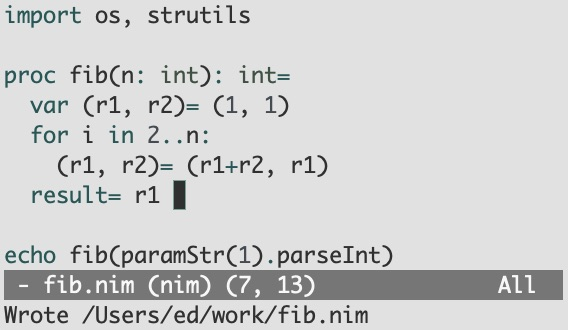
\includegraphics[width=2.60417in,height=\textheight,keepaspectratio]{figs-prefix/minibuffer.jpg}

\begin{enumerate}
\def\labelenumi{(\arabic{enumi})}
\setcounter{enumi}{2}
\tightlist
\item
  Fibonacci Function
\end{enumerate}

The figure above shows the original editor used for this tutorial.
SBEmacs uses the same style of minibuffer. In the figure you can read
the following message that was left there as the byproduct of a
\texttt{C-x\ C-s} save file command:

\begin{quote}
\texttt{Wrote\ /Users/ed/work/fib.nim}
\end{quote}

Let us test the editor. In SBEmacs, open
\texttt{\textasciitilde{}/wrk/fib.nim} with \textbf{C-x C-f}. Type the
iterative Fibonacci program from Chapter 2, then save with \textbf{C-x
C-s}. Choose \textbf{MORE → Run}, enter \texttt{5} at the arguments
prompt, and read \texttt{13} in the output window. \textbf{C-x 1}
returns to the source; \textbf{QUIT} or \textbf{C-x C-c} exits the
editor.

\subsection*{Meta keys}\label{Meta}
\addcontentsline{toc}{subsection}{Meta keys}

To issue commands in the \texttt{M-κ} form, keep the \texttt{Alt} key
down and press the \texttt{κ} key.

\begin{itemize}
\tightlist
\item
  \texttt{M-b} -- move back one word
\item
  \texttt{M-f} -- move forward one word
\item
  \texttt{M-g} -- go to the line given on the minibuffer
\item
  \texttt{M-\textgreater{}} -- go to the end of buffer
\item
  \texttt{M-\textless{}} -- go to the beginning of buffer
\end{itemize}

On a Mac, you can use Esc followed by the next key for Meta. SBEmacs
reads optional personal settings from
\texttt{\textasciitilde{}/.sbemacs/init.lisp}. For instance, the
following settings provide two alternative keys:

\begin{Shaded}
\begin{Highlighting}[]
\NormalTok{(}\KeywordTok{in{-}package}\NormalTok{ \#:sbemacs{-}user)}
\NormalTok{(global{-}set{-}key }\StringTok{"M{-}p"}\NormalTok{ (}\KeywordTok{lambda}\NormalTok{ () (run{-}key{-}as{-}typed }\StringTok{"M{-}\textless{}"}\NormalTok{)))}
\NormalTok{(global{-}set{-}key }\StringTok{"M{-}n"}\NormalTok{ (}\KeywordTok{lambda}\NormalTok{ () (run{-}key{-}as{-}typed }\StringTok{"M{-}\textgreater{}"}\NormalTok{)))}
\end{Highlighting}
\end{Shaded}

Next time you enter SBEmacs, \textbf{M-p} goes to the beginning of the
buffer and \textbf{M-n} to its end.

\subsection*{Search}\label{Search}
\addcontentsline{toc}{subsection}{Search}

If you press \texttt{C-s}, the computer enters into search mode. First,
SBEmacs prompts you for the text snippet S that you want it to find in
the current buffer. While you are still typing, the cursor jumps to the
first occurrence of the text snippet S. To repeat the search, all you
need to do is press \texttt{C-s} again. Finally, you must type
\texttt{C-r} to reverse the direction of the search.

\subsection*{Go to line}\label{Go}
\addcontentsline{toc}{subsection}{Go to line}

When you try to compile code containing errors, the compiler usually
reports the line number where the error occurred. If you press
\texttt{M-g}, SBEmacs prompts for a line number. As soon as you type the
number and press the \texttt{Enter} key, the cursor jumps to the line
where the error occurred.

\subsection*{Transport and Copy}\label{Transport}
\addcontentsline{toc}{subsection}{Transport and Copy}

To transport a region from one place to another, Nia presses
\texttt{C-Spc} to start the selection process and moves the cursor to
select the region. Then she presses \texttt{C-w} to kill her selection.
Finally, she moves the cursor to the insertion place, and presses the
\texttt{C-y} shortcut.

To copy a region, Nia presses \texttt{C-Spc} and moves the cursor to
select the region. Then she presses \texttt{M-w} to save the selection
into the kill ring. Finally, she takes the cursor to the destination
where the copy is to be inserted and issues the \texttt{C-y} command.

\chapter{The Nim computer language}\label{the-nim-computer-language}

\begin{Shaded}
\begin{Highlighting}[]
\CommentTok{\# nim c {-}d:release {-}{-}nimcache:lixo {-}o:rd.x rd.nim}
\KeywordTok{import}\NormalTok{ os}\KeywordTok{,}\NormalTok{ strutils}\KeywordTok{,}\NormalTok{ sequtils}\KeywordTok{,}\NormalTok{ sugar}
\KeywordTok{proc }\StringTok{avg}\KeywordTok{(}\NormalTok{xs}\KeywordTok{:} \DataTypeTok{seq}\KeywordTok{[}\DataTypeTok{float}\KeywordTok{]):} \DataTypeTok{float} \CommentTok{=}
  \OtherTok{result}\CommentTok{=} \DecValTok{0}\FloatTok{.}\DecValTok{0}
  \KeywordTok{var}\NormalTok{ n}\CommentTok{=} \DecValTok{0}\FloatTok{.}\DecValTok{0}
  \DataTypeTok{for}\NormalTok{ x }\CommentTok{in}\NormalTok{ xs}\KeywordTok{:}
    \OtherTok{result}\CommentTok{=} \OtherTok{result} \CommentTok{+}\NormalTok{ x}
\NormalTok{    n}\CommentTok{=}\NormalTok{ n}\CommentTok{+}\DecValTok{1}\FloatTok{.}\DecValTok{0}
  \OtherTok{result}\CommentTok{=} \OtherTok{result}\CommentTok{/}\NormalTok{n}

\KeywordTok{proc }\StringTok{main}\KeywordTok{()} \CommentTok{=}
  \DataTypeTok{if} \DataTypeTok{paramCount}\KeywordTok{()} \CommentTok{\textless{}} \DecValTok{1}\KeywordTok{:} \DataTypeTok{quit}\KeywordTok{(}\StringTok{"Usage: "} \CommentTok{\&} \DataTypeTok{paramStr}\KeywordTok{(}\DecValTok{0}\KeywordTok{)} \CommentTok{\&} \StringTok{" \textless{}filename.data\textgreater{}"}\KeywordTok{)}
  \KeywordTok{let}\NormalTok{ s }\CommentTok{=} \DataTypeTok{readFile}\KeywordTok{(}\DataTypeTok{paramStr}\KeywordTok{(}\DecValTok{1}\KeywordTok{)).}\DataTypeTok{splitWhitespace}\KeywordTok{.}\DataTypeTok{map}\KeywordTok{(}\NormalTok{x }\CommentTok{=\textgreater{}}\NormalTok{ x}\KeywordTok{.}\DataTypeTok{parseFloat}\KeywordTok{)}
  \DataTypeTok{echo} \StringTok{"Sum= "}\KeywordTok{,}\NormalTok{ s}\KeywordTok{.}\DataTypeTok{foldl}\KeywordTok{(}\NormalTok{a }\CommentTok{+}\NormalTok{ b}\KeywordTok{),} \StringTok{" / Average= "}\KeywordTok{,} \DataTypeTok{avg}\KeywordTok{(}\NormalTok{s}\KeywordTok{)}

\DataTypeTok{main}\KeywordTok{()}
\end{Highlighting}
\end{Shaded}

\begin{enumerate}
\def\labelenumi{(\arabic{enumi})}
\setcounter{enumi}{3}
\tightlist
\item
  Read and process a file
\end{enumerate}

Let us find out how many students graduate from medical schools in
California. The \texttt{grad.data} file gives the number of graduates
from each school. The \texttt{rd.nim} program prints the addition and
the average. Here is how to compile and run the program of listing 4:

\begin{verbatim}
src> nim c -o:rd.x -d:release rd.nim  # Compile 
src> cat nums.data                    # Check the data
190   45 23 34 89 96 78
97 14 17 54 345 3 42

src> ./rd.x nums.data                 # Run the program
Sum= 1127.0 / Average= 80.5
\end{verbatim}

\pagebreak

The predicate \texttt{paramCount()\ \textless{}\ 1} checks whether the
file name is present on the command line. If it is not, the program
quits with a request for the file name. In the snippet below, taken from
application 4, the \texttt{paramStr(0)} string contains the application
name.

\begin{verbatim}
  if paramCount() < 1:
    quit("Usage: " & paramStr(0) & " <filename.data>")
\end{verbatim}

The local variable \texttt{s} receives the result of a sequence of
operations concerning the file contents.

The \texttt{readFile(paramStr(1))} operation reads the file whose name
is on the command line. The \texttt{nums.data} file contains space
separated numbers that \texttt{.splitWhitespace} parses and produces a
sequence of strings.

Finally, \texttt{map(x\ =\textgreater{}\ x.parseFloat)} transforms this
sequence into floating point numbers that \texttt{foldl(a+b)} adds
together. The \texttt{avg(xs:\ seq{[}float{]})} sums the floating point
numbers together into the \texttt{result} variable and calculates the
length of the sequence into \texttt{n}. The average is
\texttt{result/n}.

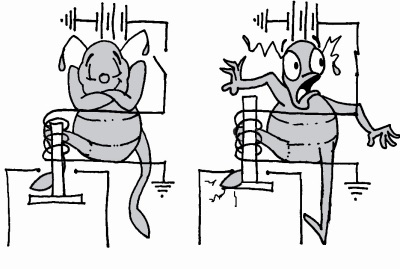
\includegraphics[width=2.60417in,height=\textheight,keepaspectratio]{figs-prefix/bugcerto.jpg}

The first computer was constructed by Konrad Zuse, a German civil
engineer, and his assistant, Ms.~Ursula Walk, née Hebekeuser. Ancient
computers, like those of Zuse and Walk, were based on relays. These are
bulky electrical devices, typically incorporating an electromagnet,
which is activated by a current in one circuit to turn on or off another
circuit. Computers made of such a contrivance were enormous, slow, and
unreliable. Therefore, on September 9th, 1945, a moth flew into one of
the relays of the Harvard Mark II computer and jammed it. From that time
on, \emph{bug} became the standard word to indicate an error that
prevents a computer from working as intended.

Due to bugs, compilers of languages like Nim and Haskell frequently
return error messages, instead of generating code and running the
corresponding programs. The Steel Bank Common Lisp language does not
interrupt code generation when the compiler spots a bug, all the same it
does issue warnings that help find the problem before the embarassment
of failure is manifest on the client's terminal.

\chapter{Comma separated values}\label{comma-separated-values}

\begin{Shaded}
\begin{Highlighting}[]
\CommentTok{\# nim c {-}d:release {-}o:csv.x {-}{-}nimcache:lixo csv.nim}
\KeywordTok{import}\NormalTok{ os}\KeywordTok{,}\NormalTok{ strutils}\KeywordTok{,}\NormalTok{ sequtils}\KeywordTok{,}\NormalTok{ sugar}

\KeywordTok{proc }\StringTok{main}\KeywordTok{()} \CommentTok{=}
  \DataTypeTok{if} \DataTypeTok{paramCount}\KeywordTok{()} \CommentTok{\textless{}} \DecValTok{1}\KeywordTok{:} \DataTypeTok{quit}\KeywordTok{(}\StringTok{"Usage: "} \CommentTok{\&} \DataTypeTok{paramStr}\KeywordTok{(}\DecValTok{0}\KeywordTok{)} \CommentTok{\&} \StringTok{"fname.data"}\KeywordTok{)}
  \KeywordTok{let}
\NormalTok{    s }\CommentTok{=} \DataTypeTok{readFile}\KeywordTok{(}\DataTypeTok{paramStr}\KeywordTok{(}\DecValTok{1}\KeywordTok{)).}\DataTypeTok{split}\KeywordTok{(}\DataTypeTok{Whitespace}\CommentTok{+}\KeywordTok{\{}\CharTok{\textquotesingle{},\textquotesingle{}}\KeywordTok{\})}
\NormalTok{    xs}\CommentTok{=}\NormalTok{ s}\KeywordTok{.}\DataTypeTok{filter}\KeywordTok{(}\NormalTok{x }\CommentTok{=\textgreater{}}\NormalTok{ x}\KeywordTok{.}\DataTypeTok{len} \CommentTok{\textgreater{}} \DecValTok{0}\KeywordTok{).}\DataTypeTok{map}\KeywordTok{(}\NormalTok{x }\CommentTok{=\textgreater{}}\NormalTok{ x}\KeywordTok{.}\DataTypeTok{parseFloat}\KeywordTok{)}
  \DataTypeTok{echo} \StringTok{"Average= "}\KeywordTok{,}\NormalTok{ xs}\KeywordTok{.}\DataTypeTok{foldl}\KeywordTok{(}\NormalTok{a}\CommentTok{+}\NormalTok{b}\KeywordTok{)}\CommentTok{/}\DataTypeTok{float}\KeywordTok{(}\NormalTok{xs}\KeywordTok{.}\DataTypeTok{len}\KeywordTok{)}

\DataTypeTok{main}\KeywordTok{()}

\CommentTok{\#[ }
\CommentTok{   Compile:  nim c {-}d:release {-}o:csv.x {-}{-}nimcache:lixo csv.nim}
\CommentTok{   src\textgreater{} cat csv.data}
\CommentTok{   190, 180, 170, 160, 120,  100}
\CommentTok{   100,90  }

\CommentTok{   src\textgreater{} ./csv.x csv.data}
\CommentTok{   Average= 138.75}
\CommentTok{]\#}
\end{Highlighting}
\end{Shaded}

The above program calculates the average of comma separated values.
Everything that comes between \texttt{\#{[}} and \texttt{{]}\#} is a
comment. In the listing above, the comments provide an example of how to
compile and use the program. Text that comes after \texttt{\#} and the
end of a line is also a comment. This second kind of comment is very
common in shell commands. The
\texttt{split(Whitespace+\{\textquotesingle{},\textquotesingle{}\})}
operation splits a string with values that can be separated by any
combination of chars that belong to the
\texttt{Whitespace+\{\textquotesingle{},\textquotesingle{}\}} set. Since
\texttt{split} produces empty \texttt{""} strings, the program applies
\texttt{filter(x\ =\textgreater{}\ x.len\ \textgreater{}\ 0)} to the
result, in order to eliminate zero-length strings from the sequence.

\section{Iterators}\label{iterators}

\begin{Shaded}
\begin{Highlighting}[]
\CommentTok{\# nim c {-}d:release {-}o:ird.x {-}{-}nimcache:lixo ird.nim}
\KeywordTok{import}\NormalTok{ os}\KeywordTok{,}\NormalTok{ strutils}

\KeywordTok{iterator }\StringTok{valid}\KeywordTok{[}\DataTypeTok{T}\KeywordTok{](}\NormalTok{a}\KeywordTok{:} \DataTypeTok{seq}\KeywordTok{[}\DataTypeTok{T}\KeywordTok{]):} \DataTypeTok{T}\CommentTok{=}
  \DataTypeTok{for}\NormalTok{ x }\CommentTok{in}\NormalTok{ a}\KeywordTok{:}
     \DataTypeTok{if}\NormalTok{ x}\KeywordTok{.}\DataTypeTok{len} \CommentTok{!=} \DecValTok{0}\KeywordTok{:} \DataTypeTok{yield}\NormalTok{ x}

\KeywordTok{proc }\StringTok{avg}\KeywordTok{(}\NormalTok{xs}\KeywordTok{:} \DataTypeTok{seq}\KeywordTok{[}\DataTypeTok{string}\KeywordTok{]):} \DataTypeTok{float} \CommentTok{=}
  \OtherTok{result}\CommentTok{=} \DecValTok{0}\FloatTok{.}\DecValTok{0}
  \KeywordTok{var}\NormalTok{ n}\CommentTok{=} \DecValTok{0}\FloatTok{.}\DecValTok{0}
  \DataTypeTok{for}\NormalTok{ x }\CommentTok{in} \DataTypeTok{valid}\KeywordTok{(}\NormalTok{xs}\KeywordTok{):}
\NormalTok{    n}\CommentTok{=}\NormalTok{ n}\CommentTok{+}\DecValTok{1}
    \OtherTok{result}\CommentTok{=} \OtherTok{result}\CommentTok{+}\NormalTok{x}\KeywordTok{.}\DataTypeTok{parseFloat}
  \OtherTok{result}\CommentTok{=} \OtherTok{result}\CommentTok{/}\NormalTok{n}

\KeywordTok{proc }\StringTok{main}\KeywordTok{()} \CommentTok{=}
  \DataTypeTok{if} \DataTypeTok{paramCount}\KeywordTok{()} \CommentTok{\textless{}} \DecValTok{1}\KeywordTok{:} \DataTypeTok{quit}\KeywordTok{(}\StringTok{"Usage: "} \CommentTok{\&} \DataTypeTok{paramStr}\KeywordTok{(}\DecValTok{0}\KeywordTok{)} \CommentTok{\&} \StringTok{" fname"}\KeywordTok{)}
  \KeywordTok{let}
\NormalTok{    s }\CommentTok{=} \DataTypeTok{readFile}\KeywordTok{(}\DataTypeTok{paramStr}\KeywordTok{(}\DecValTok{1}\KeywordTok{)).}\DataTypeTok{split}\KeywordTok{(}\DataTypeTok{Whitespace}\CommentTok{+}\KeywordTok{\{}\CharTok{\textquotesingle{},\textquotesingle{}}\KeywordTok{\})}
  \DataTypeTok{echo} \DataTypeTok{avg}\KeywordTok{(}\NormalTok{s}\KeywordTok{)}

\DataTypeTok{main}\KeywordTok{()}

\CommentTok{\#[}
\CommentTok{src\textgreater{} nim c {-}o:ird.x {-}d:release {-}{-}nimcache:./lixo ird.nim}
\CommentTok{src\textgreater{} ./ird.x csv.data}
\CommentTok{138.75}
\CommentTok{]\#}
\end{Highlighting}
\end{Shaded}

In the procedure that reads a file and splits it into an \texttt{int}
sequence, the split function generates empty strings at the end of the
file and possibly at the end of each line as well. Therefore, I designed
an iterator that feeds a \texttt{for-loop} with valid strings that can
be parsed into floats, which one can use to calculate the average of a
sequence of values.

In Nim, iterators are as easy to design as normal functions. In fact,
iterators are functions that produce values more than once. They are
defined like procedures, but the keyword \emph{iterator} replaces the
keyword \emph{proc} that defines procedures. Another difference between
iterators and functions is that an iterator uses the keyword
\emph{yield}, instead of the keyword \emph{return} to produce a value.
In general, iterators are used to feed a \texttt{for-loop} with a
sequence of values. After yielding a value, the iterator can resume the
computation to produce the next value. In the example, the iterator
\texttt{valid} yields a sequence of strings that can be parsed to
produce floating point numbers.

\chapter{Exceptions}\label{exceptions}

\begin{Shaded}
\begin{Highlighting}[]
\CommentTok{\# nim c {-}d:release {-}o:xrd.x rd.nim}

\KeywordTok{import}\NormalTok{ os}\KeywordTok{,}\NormalTok{ strutils}\KeywordTok{,}\NormalTok{ sequtils}\KeywordTok{,}\NormalTok{ sugar}
\KeywordTok{proc }\StringTok{main}\KeywordTok{()} \CommentTok{=}
  \KeywordTok{proc }\StringTok{avg}\KeywordTok{(}\NormalTok{xs}\KeywordTok{:} \DataTypeTok{seq}\KeywordTok{[}\DataTypeTok{string}\KeywordTok{]):} \DataTypeTok{float}\CommentTok{=}
     \KeywordTok{var}\NormalTok{ sm}\KeywordTok{,}\NormalTok{ n }\CommentTok{=} \DecValTok{0}\FloatTok{.}\DecValTok{0}
     \DataTypeTok{for}\NormalTok{ i}\KeywordTok{,}\NormalTok{ x }\CommentTok{in}\NormalTok{ xs}\KeywordTok{:}
       \DataTypeTok{try}\KeywordTok{:}
\NormalTok{          sm }\CommentTok{=}\NormalTok{ sm }\CommentTok{+}\NormalTok{ x}\KeywordTok{.}\DataTypeTok{strip}\KeywordTok{.}\DataTypeTok{parseFloat}
\NormalTok{          n}\CommentTok{=}\NormalTok{ n }\CommentTok{+} \DecValTok{1}\FloatTok{.}\DecValTok{0}
       \DataTypeTok{except}\KeywordTok{:} \DataTypeTok{discard}
       \DataTypeTok{finally}\KeywordTok{:} \OtherTok{result}\CommentTok{=}\NormalTok{ sm}\CommentTok{/}\NormalTok{n}

  \DataTypeTok{if} \DataTypeTok{paramCount}\KeywordTok{()} \CommentTok{\textless{}} \DecValTok{1}\KeywordTok{:} \DataTypeTok{quit}\KeywordTok{(}\StringTok{"Usage: "} \CommentTok{\&} \DataTypeTok{paramStr}\KeywordTok{(}\DecValTok{0}\KeywordTok{)} \CommentTok{\&} \StringTok{" filename"}\KeywordTok{)}
  \KeywordTok{let}\NormalTok{ xs }\CommentTok{=} \DataTypeTok{readFile}\KeywordTok{(}\DataTypeTok{paramStr}\KeywordTok{(}\DecValTok{1}\KeywordTok{)).}\DataTypeTok{split}\KeywordTok{(}\DataTypeTok{Whitespace}\CommentTok{+}\KeywordTok{\{}\CharTok{\textquotesingle{},\textquotesingle{}}\KeywordTok{\})}
  \DataTypeTok{echo} \DataTypeTok{avg}\KeywordTok{(}\NormalTok{xs}\KeywordTok{)}

\DataTypeTok{main}\KeywordTok{()}
\end{Highlighting}
\end{Shaded}

You will find \texttt{exceptions} in many languages, therefore I believe
that the above program will not pose difficulties. The \texttt{avg}
procedure does not try to eliminate invalid strings from the sequence.
Since the program is not sure that the string represents a valid
floating point number, it tries to parse it. If the \texttt{avg}
procedure fails to parse a string, the error is captured in an exception
section and immediately discarded. Let us compile and test it:

\begin{verbatim}
› nim c -o:excrd.x -d:release --nimcache:del --hints:off excrd.nim

~/nim/tutorial/src
› ./excrd.x csv.data
138.75
\end{verbatim}

\pagebreak

I defined the \texttt{avg} procedure inside the \texttt{main} procedure,
just to demonstrate that this is possible. The procedure \texttt{strip}
eliminates blanks surrounding the string, before parsing it to floating
point numbers. This is not strictly necessary, but I did it just to be
on the safe side.

\section{Ready}\label{ready}

If you installed Nim and tested the programs on the previous pages of
this tutorial, you are ready for action. Listing 5 shows an
implementation of an rpn calculator.

\pandocbounded{
\includegraphics[keepaspectratio]{figs-prefix/readyforaction.jpg}}

\begin{Shaded}
\begin{Highlighting}[]
\CommentTok{\# nim c {-}d:release {-}o:rpn.x {-}{-}nimcache:lixo rpn.nim}
\KeywordTok{import}\NormalTok{ os}\KeywordTok{,}\NormalTok{ strutils}
\KeywordTok{type }\DataTypeTok{LL}\CommentTok{=} \DataTypeTok{ref} \KeywordTok{object }\DataTypeTok{of}\CommentTok{ }\DataTypeTok{RootObj}
\NormalTok{    car}\KeywordTok{:} \DataTypeTok{float}
\NormalTok{    cdr}\KeywordTok{:} \DataTypeTok{LL}

\KeywordTok{template }\StringTok{car}\KeywordTok{(}\NormalTok{a}\KeywordTok{:}\DataTypeTok{untyped}\KeywordTok{)} \KeywordTok{:} \DataTypeTok{untyped}\CommentTok{=}
  \DataTypeTok{if}\NormalTok{ a }\CommentTok{==} \FloatTok{nil}\KeywordTok{:} \DataTypeTok{quit}\KeywordTok{(}\StringTok{"Empty stack"}\KeywordTok{)}
  \DataTypeTok{else}\KeywordTok{:}\NormalTok{ a}\KeywordTok{.}\DataTypeTok{car}
\KeywordTok{template }\StringTok{\textasciigrave{}\textgreater{}\textgreater{}\textasciigrave{}}\CommentTok{ }\KeywordTok{(}\NormalTok{a}\KeywordTok{,}\NormalTok{b}\KeywordTok{:}\DataTypeTok{untyped}\KeywordTok{):} \DataTypeTok{untyped}\CommentTok{=} \DataTypeTok{LL}\KeywordTok{(}\NormalTok{car}\KeywordTok{:}\NormalTok{ a}\KeywordTok{,}\NormalTok{ cdr}\KeywordTok{:}\NormalTok{ b}\KeywordTok{)}

\KeywordTok{proc }\StringTok{eval}\KeywordTok{(}\NormalTok{x}\KeywordTok{:} \DataTypeTok{string}\KeywordTok{,}\NormalTok{ s}\KeywordTok{:} \KeywordTok{var} \DataTypeTok{LL}\KeywordTok{)}\CommentTok{=}
  \DataTypeTok{try}\KeywordTok{:}\NormalTok{ s}\CommentTok{=}\NormalTok{ x}\KeywordTok{.}\DataTypeTok{strip}\KeywordTok{.}\DataTypeTok{parseFloat} \CommentTok{\textgreater{}\textgreater{}}\NormalTok{ s}
  \DataTypeTok{except}\KeywordTok{:}
    \DataTypeTok{case}\NormalTok{  x}\KeywordTok{:}
      \CommentTok{of} \StringTok{"+"}\KeywordTok{:}\NormalTok{ s}\CommentTok{=} \KeywordTok{(}\DataTypeTok{car}\NormalTok{ s}\KeywordTok{)} \CommentTok{+} \KeywordTok{(}\DataTypeTok{car}\NormalTok{ s}\KeywordTok{.}\DataTypeTok{cdr}\KeywordTok{)} \CommentTok{\textgreater{}\textgreater{}}\NormalTok{ s}\KeywordTok{.}\DataTypeTok{cdr}\KeywordTok{.}\DataTypeTok{cdr}
      \CommentTok{of} \StringTok{"x"}\KeywordTok{:}\NormalTok{ s}\CommentTok{=} \KeywordTok{(}\DataTypeTok{car}\NormalTok{ s}\KeywordTok{)} \CommentTok{*} \KeywordTok{(}\DataTypeTok{car}\NormalTok{ s}\KeywordTok{.}\DataTypeTok{cdr}\KeywordTok{)} \CommentTok{\textgreater{}\textgreater{}}\NormalTok{ s}\KeywordTok{.}\DataTypeTok{cdr}\KeywordTok{.}\DataTypeTok{cdr}
      \CommentTok{of} \StringTok{"/"}\KeywordTok{:}\NormalTok{ s}\CommentTok{=} \KeywordTok{(}\DataTypeTok{car}\NormalTok{ s}\KeywordTok{.}\DataTypeTok{cdr}\KeywordTok{)} \CommentTok{/} \KeywordTok{(}\DataTypeTok{car}\NormalTok{ s}\KeywordTok{)} \CommentTok{\textgreater{}\textgreater{}}\NormalTok{ s}\KeywordTok{.}\DataTypeTok{cdr}\KeywordTok{.}\DataTypeTok{cdr}
      \CommentTok{of} \StringTok{"{-}"}\KeywordTok{:}\NormalTok{ s}\CommentTok{=} \KeywordTok{(}\DataTypeTok{car}\NormalTok{ s}\KeywordTok{.}\DataTypeTok{cdr}\KeywordTok{)} \CommentTok{{-}} \KeywordTok{(}\DataTypeTok{car}\NormalTok{ s}\KeywordTok{)} \CommentTok{\textgreater{}\textgreater{}}\NormalTok{ s}\KeywordTok{.}\DataTypeTok{cdr}\KeywordTok{.}\DataTypeTok{cdr}
      \CommentTok{of} \StringTok{"neg"}\KeywordTok{:}\NormalTok{ s}\CommentTok{=} \CommentTok{{-}}\KeywordTok{(}\DataTypeTok{car}\NormalTok{ s}\KeywordTok{)} \CommentTok{\textgreater{}\textgreater{}}\NormalTok{ s}\KeywordTok{.}\DataTypeTok{cdr}
      \DataTypeTok{else}\KeywordTok{:} \DataTypeTok{quit}\KeywordTok{(}\StringTok{"Error in eval"}\KeywordTok{)}

\KeywordTok{var}\NormalTok{ stk}\KeywordTok{:} \DataTypeTok{LL} \CommentTok{=} \FloatTok{nil}
\DataTypeTok{for}\NormalTok{ i }\CommentTok{in} \DataTypeTok{1} \KeywordTok{..} \DataTypeTok{paramCount}\KeywordTok{():} \DataTypeTok{eval}\KeywordTok{(}\DataTypeTok{paramStr}\KeywordTok{(}\NormalTok{i}\KeywordTok{),}\NormalTok{ stk}\KeywordTok{)}
\DataTypeTok{while}\NormalTok{ stk }\CommentTok{!=} \FloatTok{nil}\KeywordTok{:}
  \DataTypeTok{echo}\NormalTok{ stk}\KeywordTok{.}\DataTypeTok{car}
\NormalTok{  stk}\CommentTok{=}\NormalTok{ stk}\KeywordTok{.}\DataTypeTok{cdr}
\end{Highlighting}
\end{Shaded}

\begin{enumerate}
\def\labelenumi{(\arabic{enumi})}
\setcounter{enumi}{4}
\tightlist
\item
  Implementation of an rpn calculator
\end{enumerate}

\pagebreak

Before trying to understand the program of listing 5, let us see how to
use it. The program is an emulator of the famous hp calculators.

In pre-algebra, students learn to place arithmetic operators, such as
(+, -, × and ÷), between their operands; e.g.~345+47. However, when
doing sums and subtractions on paper, they stack the operands.

\pandocbounded{
\includegraphics[keepaspectratio]{figs-prefix/stackshark.jpg}}

\begin{enumerate}
\def\labelenumi{(\arabic{enumi})}
\setcounter{enumi}{5}
\tightlist
\item
  Adding to numbers
\end{enumerate}

Accountants and engineers use the operator itself to separate the result
from the operands, instead of drawing a line under the last operand.

\pandocbounded{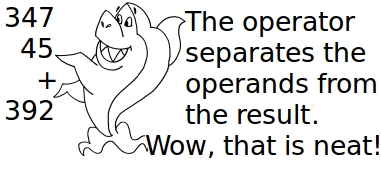
\includegraphics[keepaspectratio]{figs-prefix/neatsum.jpg}}

Here is the story of a Texan who went on vacation to a beach in Mexico.
While he was freely dallying with the local beauties, unbeknownst to him
a blackmailer took some rather incriminating photos.

After a week long gallivanting, the Texan returns to his ranch in a
small town near Austin. Arriving at his door shortly after is the
blackmailer full of bad intentions.

Unaware of any malice, the Texan allows the so called photographer to
enter and sit in front of his desk. Without delay, the blackmailer
spread out a number of photos on the desk, along with his demands: ``For
the photo in front of the hotel, that will cost you \$25,320.00. Well,
the one on the beach that's got to be \$ 56,750.00. Finally, this
definitively I can't let go for less than \$136,000.00.''

Once finished with his presentation, the blackmailer snaps up the
photos, and looks to the Texan with a sinister grin, awaiting his reply.

Delighted with the selection of pictures, the Texan in an elated voice
says: ``I thought I would have no recollection of my wonderful time. I
want 3 copies of the hotel shot, half a dozen of the beach. And the last
one, I need two copies for myself, and please, send one to my ex-wife.
Make sure you leave me your contact details; I might need some more.

In order to calculate how much the Texan should pay his supposed
blackmailer, his bookkeeper needs to perform the following operations:

\begin{verbatim}
3×25320+6×56750+2×136000+136000 
\end{verbatim}

Below, you can see how the Texan's bookkeeper calculates the
blackmailer's payment with the calculator from listing 5.

\begin{verbatim}
src> ./rpn.x 3 25320 x  6 56750 x + 3 136000 x +
824460.0
\end{verbatim}

\section{Nimscript}\label{nimscript}

Up to this point, you have used the command line to call the Nim
compiler. A better approach to manage compilation is to create a
nimscript as the one suggested by SolitudeSF and RSDuck.

\begin{Shaded}
\begin{Highlighting}[]
\CommentTok{\#!/usr/bin/env {-}S nim {-}{-}hints:off}
\NormalTok{mode }\CommentTok{=} \DataTypeTok{ScriptMode.Silent}
\DataTypeTok{from} \DataTypeTok{os} \KeywordTok{import}\NormalTok{ \textasciigrave{}}\CommentTok{/}\NormalTok{\textasciigrave{}}
\DataTypeTok{if} \DataTypeTok{paramCount}\KeywordTok{()} \CommentTok{\textgreater{}} \DecValTok{2} \CommentTok{and} \DataTypeTok{fileExists}\KeywordTok{(}\DataTypeTok{paramStr}\KeywordTok{(}\DecValTok{3}\KeywordTok{)} \CommentTok{\&} \StringTok{".nim"}\KeywordTok{):} 
  \KeywordTok{let}
\NormalTok{    app }\CommentTok{=} \DataTypeTok{paramStr}\KeywordTok{(}\DecValTok{3}\KeywordTok{)}
\NormalTok{    src }\CommentTok{=}\NormalTok{ app }\CommentTok{\&} \StringTok{".nim"}
\NormalTok{    exe }\CommentTok{=}\NormalTok{ app }\CommentTok{\&} \StringTok{".x"}
\NormalTok{    c }\CommentTok{=} \StringTok{"nim c {-}{-}hints:off {-}{-}nimcache:xx {-}d:danger {-}o:"}

  \DataTypeTok{exec}\NormalTok{ c }\CommentTok{\&}\NormalTok{ exe }\CommentTok{\&} \StringTok{" "} \CommentTok{\&}\NormalTok{ src}
  \DataTypeTok{echo}\NormalTok{ c }\CommentTok{\&}\NormalTok{ exe }\CommentTok{\&} \StringTok{" "} \CommentTok{\&}\NormalTok{ src}
  \DataTypeTok{mvFile}\NormalTok{ exe}\KeywordTok{,} \StringTok{"bin"} \CommentTok{/}\NormalTok{ exe}
\DataTypeTok{else}\KeywordTok{:} \DataTypeTok{echo} \StringTok{"Usage: ./build.nims \textless{}app without extension\textgreater{}"}
\end{Highlighting}
\end{Shaded}

\begin{enumerate}
\def\labelenumi{(\arabic{enumi})}
\setcounter{enumi}{6}
\tightlist
\item
  A Nimscript for building small applications
\end{enumerate}

A nimscript contains rules for building programs and managing files. The
rules state how to make or remake certain files that are called the rule
targets. A variable in nimscript has the same meaning as in Nim,
therefore variables are ids defined in a script to represent a string of
text, called value. When you call a script, for instance
\texttt{./build.nims\ rpn}, to build a program, you can specify the
value of the \texttt{app} variable through \texttt{paramStr(3)}.

In the script of listing 7, the variables \texttt{src}, \texttt{exe} and
\texttt{c} contain parts of the command line that will be passed to
\texttt{exec} and build the application. The first line of the script,
which is prefixed by \texttt{\#!} (she bang), will call the \texttt{nim}
compiler to execute the script. Thus, the command below executes the
\texttt{build.nims} of the previous page and compiles the
\texttt{rpn.nim} program.

\begin{Shaded}
\begin{Highlighting}[]
\NormalTok{src› chmod a+x build.nims}
\NormalTok{src› ./build.nims rpn}
\NormalTok{CC: rpn.nim}
\NormalTok{src\textgreater{} }
\end{Highlighting}
\end{Shaded}

In the above example, the \texttt{chmod} command will give permission to
execute the script.

When you call \texttt{./build.nims\ rpn} from the command line, the
\texttt{app} variable receives the \texttt{rpn} value, which will be
expanded into the recipe below:

\begin{Shaded}
\begin{Highlighting}[]
\DataTypeTok{exec} \DataTypeTok{nim}\NormalTok{ c }\CommentTok{{-}{-}}\NormalTok{hints}\KeywordTok{:}\FloatTok{off} \CommentTok{{-}{-}}\NormalTok{nimcache}\KeywordTok{:}\NormalTok{xx }\CommentTok{{-}}\NormalTok{d}\KeywordTok{:}\NormalTok{danger }\CommentTok{{-}}\NormalTok{o}\KeywordTok{:}\NormalTok{rpn}\KeywordTok{.}\DataTypeTok{x}\NormalTok{ rpn}\KeywordTok{.}\DataTypeTok{nim}
\end{Highlighting}
\end{Shaded}

The result of the expansion will compile the \texttt{rpn.nim} program,
and output the \texttt{rpn.x} executable code.

\section{Linked List}\label{linked-list}

Let us understand the program of listing 5. A list is a sequence of
connected links, like a chain. In listing 5, links are represented by
the \texttt{LL(car:\ a,\ cdr:\ b)} type.

\begin{verbatim}
CL-USER> (draw-cons-tree::draw-tree (list 2 4 8 16))
[o|o]---[o|o]---[o|o]---[o|/]
 |       |       |       |
 2       4       8       16
\end{verbatim}

In the Lisp community, where the idea of linked list gained momentum,
links have two parts, the \texttt{car} field contains the datum and the
\texttt{cdr} field contains the address of the next link. In order to
facilitate the creation of a sequence of links, listing 5 defines the
\texttt{a\ \textgreater{}\textgreater{}\ b} template, which assigns the
\texttt{a} value to the \texttt{car} field, and the \texttt{b} address
to the \texttt{cdr} field.

The \texttt{eval(x:\ string,\ s:\ var\ LL)} tries to parse \texttt{x}
into a float pointing number. If it succeeds, the result is linked to
the \texttt{stk} var. If \texttt{x} does not parse, \texttt{eval} checks
whether it is an arithmetic operator through the \texttt{except} branch
of the case-command. Let us suppose that it is the \texttt{"+"}
operator. In this case, \texttt{"+"} fetches its two arguments from the
stack, adds them, and pushes the result to the stack. The first argument
is given by the \texttt{(car\ s)} template, and the second argument is
given by \texttt{(car\ s.cdr)}.

In the \texttt{eval(x:\ string,\ s:var\ LL)} procedure, \texttt{s} is
declared as \texttt{var}, which means that it can destructively assign
values to the \texttt{stk} var, in the \texttt{eval(paramStr(i),\ stk)}
call.

\section{Symbolic computation}\label{symbolic-computation}

The concept of linked list was introduced in the Lisp language for
symbolic computation, i.e., modeling mechanical machinery in Computer
Aid Design, performing algebraic manipulations and constructing
syntactical trees for analysing natural, etc. The name list give the
misleading impression that this data structure represent mainly
sequences. In fact, lists represent trees.

I will make a few statements about lists that you will accept for its
face value. As you gain experience with computers, you will see that
they are indeed true. The first statement is that lists represents
trees.

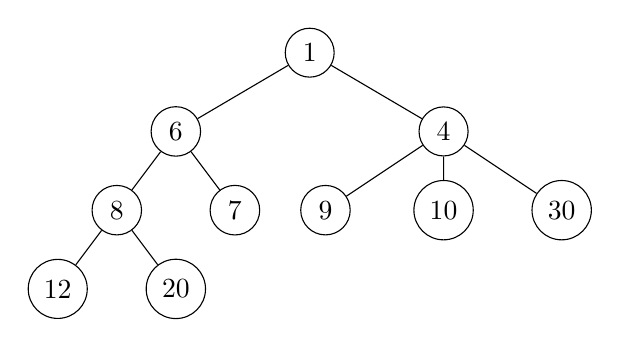
\begin{tikzpicture}
 \node [circle,draw]{1} [level distance=10mm,sibling distance=34mm]
child { node [circle,draw]{6} [level distance=10mm ,sibling distance=15mm]
child {node [circle,draw] {8}
child {node [circle,draw] {12}}
child {node [circle,draw]{20}}}
child {node [circle,draw]{7}}
}
child {node [circle,draw] {4} [level distance=10mm ,sibling distance=15mm]
child {node [circle,draw] {9}}
child {node [circle,draw] {10}}
child {node [circle,draw]{30}}
};
\end{tikzpicture}

\begin{enumerate}
\def\labelenumi{(\arabic{enumi})}
\setcounter{enumi}{7}
\tightlist
\item
  A small tree
\end{enumerate}

Consider the tree on figure 8. You can represent each node as list,
where the first element is the node label, and the other elements are
branches. Therefore, the subtree that branches from node 8 is
represented thus:

\begin{Shaded}
\begin{Highlighting}[]
\NormalTok{(}\DecValTok{8} \DecValTok{12} \DecValTok{20}\NormalTok{)}
\end{Highlighting}
\end{Shaded}

The subtree that starts at node 6 has two branches, and can be
represented as shown below:

\begin{Shaded}
\begin{Highlighting}[]
\NormalTok{(}\DecValTok{6}\NormalTok{ (}\DecValTok{8} \DecValTok{12} \DecValTok{20}\NormalTok{) }\DecValTok{7}\NormalTok{)}
\end{Highlighting}
\end{Shaded}

The list representation for the whole tree of figure 8 is shown below:

\begin{Shaded}
\begin{Highlighting}[]
\NormalTok{(}\DecValTok{1}\NormalTok{ (}\DecValTok{6}\NormalTok{ (}\DecValTok{8} \DecValTok{12} \DecValTok{20}\NormalTok{)}
      \DecValTok{7}\NormalTok{)}
\NormalTok{   (}\DecValTok{4}\NormalTok{ (}\DecValTok{9} \DecValTok{10} \DecValTok{30}\NormalTok{)))}
\end{Highlighting}
\end{Shaded}

The best way to go through such a tree is by using recursion together
with the car/cdr selectors, as you will see in chapter
\ref{chp:Lisp-like-macro}.

\chapter{Web pages}\label{web-pages}

In this chapter, you will learn how to write a web application in pure
Nim. But firstly, let us learn what cloud computing is.

Cloud computing is an Internet based computer that provides shared
processing on demand for those people connected to a service provider.
When a company adheres to cloud computing, it avoids infrastructure
costs, such as purchasing servers, and keeping them in working order.

At the time of this writing, fees for cloud computing can be pretty
steep. However, one can hire a normal hosting service and use it for
creating pages that are able to run quite interesting applications.

When you hire a hosting service, you will receive a user name and will
be requested to buy a domain name. Let us assume that a resident owns
the \texttt{medicina.tips} domain, where \emph{medicina} means health
care in Latin. The domain may be any sequence of chars, but it is a good
idea to choose names that raise interest in Web users. Since doctors
usually know some Latin, if one wants to offer expert medical
consultancy, \texttt{medicina.tips} is a good name. Now that our
resident physician has a user name and a domain, he must install a few
programs in his cloud machine. Here is how he enters the shell:

\begin{Shaded}
\begin{Highlighting}[]
\NormalTok{\textasciitilde{}$ ssh {-}p2222 nia@medicina.tips}
\NormalTok{nia@medicina.tips\textquotesingle{}s password: ***}
\end{Highlighting}
\end{Shaded}

The 2222 port is used in the secure shell protocol that connects the
administrator of the page to the cloud computer. The administrator needs
a password to complete the connection.

\begin{Shaded}
\begin{Highlighting}[]
\NormalTok{Last login: Sep 25 18:03:00 2022 from 179.155.71.6}
\NormalTok{\textasciitilde{}$ cd public\_html}
\NormalTok{\textasciitilde{}/public\_html$ mkdir nim}
\NormalTok{\textasciitilde{}/public\_html$ cd nim}
\NormalTok{\textasciitilde{}/public\_html/nim$ echo "Addhandler cgi{-}script .cgi .s .k .n" \textgreater{} .htaccess}
\end{Highlighting}
\end{Shaded}

The \texttt{.htaccess} file specifies an extension for running Nim
applications on the web. It is possible that, in your cloud machine, the
protocol for running Nim programs is different from what is described in
this tutorial. You must ask the vendor for details.

\begin{Shaded}
\begin{Highlighting}[]
\CommentTok{\# File: web.nim}
\KeywordTok{import}\NormalTok{ strutils}\KeywordTok{,}\NormalTok{ os}\KeywordTok{,}\NormalTok{ strscans}\KeywordTok{,}\NormalTok{ unicode}\KeywordTok{,}\NormalTok{ uri}

\KeywordTok{let}\NormalTok{ input }\CommentTok{=} \DataTypeTok{open}\KeywordTok{(}\StringTok{"rage.md"}\KeywordTok{)}
\KeywordTok{let}\NormalTok{ form }\CommentTok{=} \StringTok{"""}
\StringTok{   \textless{}form name=\textquotesingle{}form\textquotesingle{} method=\textquotesingle{}get\textquotesingle{}\textgreater{}}
\StringTok{       Visitor: \textless{}input type=\textquotesingle{}type=\textquotesingle{}text\textquotesingle{} name=\textquotesingle{}$\#\textquotesingle{}/\textgreater{}}
\StringTok{    \textless{}/form\textgreater{} \textless{}br/\textgreater{}}
\StringTok{  """}

\DataTypeTok{echo} \StringTok{"Content{-}type: text/html}\NormalTok{\textbackslash{}n\textbackslash{}n}\StringTok{\textless{}html\textgreater{}"}
\DataTypeTok{echo} \StringTok{"""}
\StringTok{  \textless{}head\textgreater{}}
\StringTok{    \textless{}meta http{-}equiv= \textquotesingle{}Content{-}type\textquotesingle{}}
\StringTok{      content= \textquotesingle{}text/html; charset=utf{-}8\textquotesingle{} /\textgreater{}}
\StringTok{  \textless{}/head\textgreater{}}
\StringTok{\textless{}body\textgreater{}  }
\StringTok{"""}

\KeywordTok{proc }\StringTok{tl}\KeywordTok{(}\NormalTok{input}\KeywordTok{:} \DataTypeTok{string}\KeywordTok{;}\NormalTok{ match}\KeywordTok{:} \KeywordTok{var} \DataTypeTok{string}\KeywordTok{,}\NormalTok{ start}\KeywordTok{:} \DataTypeTok{int}\KeywordTok{):} \DataTypeTok{int} \CommentTok{=}
\NormalTok{  match }\CommentTok{=}\NormalTok{ input}\KeywordTok{[}\DataTypeTok{start} \KeywordTok{..}\NormalTok{ input}\KeywordTok{.}\DataTypeTok{high}\KeywordTok{]}
  \OtherTok{result} \CommentTok{=} \DataTypeTok{max}\KeywordTok{(}\DecValTok{1}\KeywordTok{,}\NormalTok{ input}\KeywordTok{.}\DataTypeTok{len} \CommentTok{{-}}\NormalTok{ start}\KeywordTok{)}

\KeywordTok{var}\NormalTok{ html}\KeywordTok{:} \DataTypeTok{string}
\DataTypeTok{for}\NormalTok{ line }\CommentTok{in}\NormalTok{ input}\KeywordTok{.}\DataTypeTok{lines}\KeywordTok{:}
  \DataTypeTok{if} \DataTypeTok{scanf}\KeywordTok{(}\NormalTok{line}\KeywordTok{,} \StringTok{"\#\# $\{tl\}"}\KeywordTok{,}\NormalTok{ html}\KeywordTok{):} \DataTypeTok{echo} \StringTok{"\textless{}h2\textgreater{} $1 \textless{}/h2\textgreater{}"} \CommentTok{\%} \DataTypeTok{html} 
  \DataTypeTok{elif} \DataTypeTok{scanf}\KeywordTok{(}\NormalTok{line}\KeywordTok{,} \StringTok{"\# $\{tl\}"}\KeywordTok{,}\NormalTok{ html}\KeywordTok{):} \DataTypeTok{echo} \StringTok{"\textless{}h1\textgreater{}$1\textless{}/h1\textgreater{}"} \CommentTok{\%}\NormalTok{ html}
  \DataTypeTok{elif} \DataTypeTok{scanf}\KeywordTok{(}\NormalTok{line}\KeywordTok{,} \StringTok{"in: $\{tl\}"}\KeywordTok{,}\NormalTok{ html}\KeywordTok{):} \DataTypeTok{echo} \DataTypeTok{form} \CommentTok{\%}\NormalTok{ html}
  \DataTypeTok{elif} \DataTypeTok{scanf}\KeywordTok{(}\NormalTok{line}\KeywordTok{,} \StringTok{"$\{tl\}"}\KeywordTok{,}\NormalTok{ html}\KeywordTok{):} \DataTypeTok{echo} \StringTok{"$\#\textless{}br/\textgreater{}"} \CommentTok{\%}\NormalTok{ html}

\KeywordTok{let}\NormalTok{ qs }\CommentTok{=} \DataTypeTok{getEnv}\KeywordTok{(}\StringTok{"QUERY\_STRING"}\KeywordTok{,} \StringTok{"none"}\KeywordTok{)}
\DataTypeTok{if}\NormalTok{ qs }\CommentTok{!=} \StringTok{"none"} \CommentTok{and}\NormalTok{ qs}\KeywordTok{.}\DataTypeTok{len} \CommentTok{\textgreater{}} \DecValTok{0}\KeywordTok{:}
  \KeywordTok{let}\NormalTok{ vs }\CommentTok{=} \DataTypeTok{open}\KeywordTok{(}\StringTok{"visitors.txt"}\KeywordTok{,}\NormalTok{ fmAppend}\KeywordTok{)}
  \DataTypeTok{if} \DataTypeTok{scanf}\KeywordTok{(}\NormalTok{qs}\KeywordTok{,} \StringTok{"N=$\{tl\}"}\KeywordTok{,}\NormalTok{ html}\KeywordTok{):}
     \KeywordTok{let}\NormalTok{ n}\CommentTok{=} \StringTok{"$\#"} \CommentTok{\%}\NormalTok{ html}
     \DataTypeTok{if}\NormalTok{ n }\CommentTok{!=} \StringTok{""} \CommentTok{and} \CommentTok{not} \DataTypeTok{isSpace}\KeywordTok{(}\NormalTok{n}\KeywordTok{):} \DataTypeTok{write}\KeywordTok{(}\NormalTok{vs}\KeywordTok{,}\NormalTok{ n}\KeywordTok{.}\DataTypeTok{decodeUrl}\KeywordTok{(}\FloatTok{true}\KeywordTok{)} \CommentTok{\&} \StringTok{"}\NormalTok{\textbackslash{}n}\StringTok{"}\KeywordTok{)}
\NormalTok{  vs}\KeywordTok{.}\DataTypeTok{close}

\KeywordTok{let}\NormalTok{ inputVisitors}\CommentTok{=} \DataTypeTok{open}\KeywordTok{(}\StringTok{"visitors.txt"}\KeywordTok{)}
\DataTypeTok{for}\NormalTok{ line }\CommentTok{in}\NormalTok{ inputVisitors}\KeywordTok{.}\DataTypeTok{lines}\KeywordTok{:} \DataTypeTok{echo}\NormalTok{ line}\CommentTok{\&}\StringTok{"\textless{}br/\textgreater{}"}
\NormalTok{inputVisitors}\KeywordTok{.}\DataTypeTok{close}
\DataTypeTok{echo} \StringTok{"\textless{}/body\textgreater{}\textless{}/html\textgreater{}"}
\NormalTok{input}\KeywordTok{.}\DataTypeTok{close}
\end{Highlighting}
\end{Shaded}

\begin{enumerate}
\def\labelenumi{(\arabic{enumi})}
\setcounter{enumi}{8}
\tightlist
\item
  A web application
\end{enumerate}

The idea is to run the program of listing 9 from the Internet. However,
it is not enough to compile the program in your home computer and
install it in the cloud machine, since the two computers are likely
different. You need to install a tool chain of the cloud computer in
your home computer, then use the \texttt{nim.cfg} file to inform where
it is located:

\begin{Shaded}
\begin{Highlighting}[]
\NormalTok{amd64}\KeywordTok{.}\DataTypeTok{linux}\KeywordTok{.}\DataTypeTok{gcc}\KeywordTok{.}\DataTypeTok{path}\KeywordTok{:}\StringTok{"/usr/local/Cellar/musl{-}cross/0.9.8/bin"}
\NormalTok{amd64}\KeywordTok{.}\DataTypeTok{linux}\KeywordTok{.}\DataTypeTok{gcc}\KeywordTok{.}\DataTypeTok{exe}\KeywordTok{:}\StringTok{"x86\_64{-}linux{-}musl{-}gcc"}
\NormalTok{amd64}\KeywordTok{.}\DataTypeTok{linux}\KeywordTok{.}\DataTypeTok{gcc}\KeywordTok{.}\DataTypeTok{linkerexe}\KeywordTok{:}\StringTok{"x86\_64{-}linux{-}musl{-}gcc"}
\end{Highlighting}
\end{Shaded}

\begin{enumerate}
\def\labelenumi{(\arabic{enumi})}
\setcounter{enumi}{9}
\tightlist
\item
  The \texttt{nim.cfg} file
\end{enumerate}

\subsection*{Script for cross compiling}\label{ScriptFor}
\addcontentsline{toc}{subsection}{Script for cross compiling}

Of course, this \texttt{nim.cfg} file refers to my tool chain
installation. If necessary, ask for the help of a computer science major
to install an adequate tool chain.

The task of compiling a web application in your home computer is called
cross compilation, and needs a special script.

\begin{Shaded}
\begin{Highlighting}[]
\CommentTok{\#!/usr/bin/env {-}S nim {-}{-}hints:off}
\NormalTok{mode }\CommentTok{=} \DataTypeTok{ScriptMode.Silent}
\DataTypeTok{if} \DataTypeTok{paramCount}\KeywordTok{()} \CommentTok{\textgreater{}} \DecValTok{2} \CommentTok{and} \DataTypeTok{fileExists}\KeywordTok{(}\DataTypeTok{paramStr}\KeywordTok{(}\DecValTok{3}\KeywordTok{)} \CommentTok{\&} \StringTok{".nim"}\KeywordTok{):} 
  \KeywordTok{let}
\NormalTok{    app }\CommentTok{=} \DataTypeTok{paramStr}\KeywordTok{(}\DecValTok{3}\KeywordTok{)}
\NormalTok{    src }\CommentTok{=}\NormalTok{ app }\CommentTok{\&} \StringTok{".nim"}
\NormalTok{    exe }\CommentTok{=} \StringTok{"nim"} \CommentTok{\&}\NormalTok{ app }\CommentTok{\&} \StringTok{".k "}
\NormalTok{    c }\CommentTok{=} \StringTok{"nim c {-}{-}nimcache:xx {-}{-}os:linux {-}{-}cpu:amd64 {-}d:release {-}o:"}
\NormalTok{    cc}\CommentTok{=} \StringTok{" {-}{-}passL:}\NormalTok{\textbackslash{}"}\StringTok{{-}static}\NormalTok{\textbackslash{}"}\StringTok{"}
  \DataTypeTok{exec}\NormalTok{ c }\CommentTok{\&}\NormalTok{ exe }\CommentTok{\&} \StringTok{" "} \CommentTok{\&}\NormalTok{ cc }\CommentTok{\&} \StringTok{" "} \CommentTok{\&}\NormalTok{ src}
  \DataTypeTok{echo}\NormalTok{ c }\CommentTok{\&}\NormalTok{ exe }\CommentTok{\&} \StringTok{" "} \CommentTok{\&}\NormalTok{ cc }\CommentTok{\&} \StringTok{" "} \CommentTok{\&}\NormalTok{ src}
\DataTypeTok{else}\KeywordTok{:} \DataTypeTok{echo} \StringTok{"Usage: ./build.nims \textless{}app without extension\textgreater{}"}
\end{Highlighting}
\end{Shaded}

\begin{enumerate}
\def\labelenumi{(\arabic{enumi})}
\setcounter{enumi}{10}
\tightlist
\item
  Script for cross compilation: \texttt{cross.nims}
\end{enumerate}

It is advisable to place the three components of the cross compilation
in the same directory, say \texttt{\textasciitilde{}/nim/os}. Then you
can use the script to compile the program, as shown below.

\begin{Shaded}
\begin{Highlighting}[]
\NormalTok{\textasciitilde{}/nim/os› ./cross.nims web}
\NormalTok{Hint: used config file \textquotesingle{}/etc/nim/nim.cfg\textquotesingle{} [Conf]}
\NormalTok{Hint: used config file \textquotesingle{}/Users/ed/nim/os/nim.cfg\textquotesingle{} [Conf]}
\NormalTok{Hint: web [Processing]}
\NormalTok{CC: stdlib\_os.nim}
\NormalTok{CC: web.nim}
\NormalTok{Hint:  [Link]}
\NormalTok{Hint: operation successful (Release Build) [SuccessX]}
\NormalTok{nim c {-}{-}nimcache:xx {-}{-}os:linux {-}{-}cpu:amd64\textbackslash{}}
\NormalTok{  {-}d:release {-}o:nimweb.n   {-}{-}passL:"{-}static" web.nim}
\end{Highlighting}
\end{Shaded}

The last step is to send the compiled program to the cloud machine,
which can be done through the \texttt{scp} command, a version of the
\texttt{cp} command that can send files from a point in the cloud to
another.

\begin{Shaded}
\begin{Highlighting}[]
\NormalTok{scp {-}P2222 nimweb.n strue028@medicina.tips:\textasciitilde{}/public\_html/nim/}
\end{Highlighting}
\end{Shaded}

\subsection*{How the application works}\label{HowWorks}
\addcontentsline{toc}{subsection}{How the application works}

Let us analyse how the application of listing 9 works. The
\texttt{rage.md} file contain a few lines of a poem without any
structure. The idea is to write it in html, so the poem can be
visualized through a web browser. The \texttt{open} command does what
its name indicates, it opens a file and place the descriptor in the
\texttt{input} variable.

The \texttt{input.lines} iterator feeds the file lines to the code that
will format them. Basically, if the line has a sharp \texttt{"\#"}
prefix, it is marked as title.

\pandocbounded{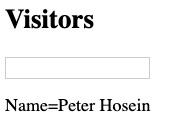
\includegraphics[keepaspectratio]{figs-prefix/webpage.jpg}}

If a visitor types his or her name on the \texttt{Name} field, the name
is captured by the \texttt{"QUERY\_STRING"} variable and saved in the
\texttt{visitors.txt} file.

I hope you will be able to modify the program of listing 9, and use its
concept in your own applications. You can use the web for opinion
polling, collecting and processing data, e-commerce, or just to spread
your ideas. In the last case, you can use Nim to count how many people
visited your site.

\chapter{Macros}\label{macros}

\begin{Shaded}
\begin{Highlighting}[]
\CommentTok{\# ./build.nims quoteLoop}
\KeywordTok{import}\NormalTok{ macros}\KeywordTok{,}\NormalTok{ strutils}\KeywordTok{,}\NormalTok{ os}

\KeywordTok{macro }\StringTok{magicWord}\KeywordTok{(}\NormalTok{statments}\KeywordTok{:} \DataTypeTok{untyped}\KeywordTok{):} \DataTypeTok{untyped} \CommentTok{=}
    \DocumentationTok{\#\# Designed by Steve Kellock}
    \OtherTok{result} \CommentTok{=}\NormalTok{ statments}
    \DataTypeTok{for}\NormalTok{ st }\CommentTok{in}\NormalTok{ statments}\KeywordTok{:}
          \DataTypeTok{for}\NormalTok{ node }\CommentTok{in}\NormalTok{ st}\KeywordTok{:}
                \DataTypeTok{if}\NormalTok{ node}\KeywordTok{.}\DataTypeTok{kind} \CommentTok{==}\NormalTok{ nnkStrLit}\KeywordTok{:}
\NormalTok{                     node}\KeywordTok{.}\DataTypeTok{strVal} \CommentTok{=}\NormalTok{ node}\KeywordTok{.}\DataTypeTok{strVal} \CommentTok{\&} \StringTok{", Please."}

\KeywordTok{macro }\StringTok{rpt}\KeywordTok{(}\NormalTok{ix}\KeywordTok{:} \DataTypeTok{untyped}\KeywordTok{,}\NormalTok{ cnt}\KeywordTok{:} \DataTypeTok{int}\KeywordTok{,}\NormalTok{ statements}\KeywordTok{:} \DataTypeTok{untyped}\KeywordTok{)}\CommentTok{=}
  \DataTypeTok{quote} \DataTypeTok{do}\KeywordTok{:}
    \DataTypeTok{for}\NormalTok{ \textasciigrave{}ix\textasciigrave{} }\CommentTok{in} \DecValTok{1}\KeywordTok{..}\NormalTok{\textasciigrave{}cnt\textasciigrave{}}\KeywordTok{:}
\NormalTok{      \textasciigrave{}statements\textasciigrave{}}

\DataTypeTok{rpt}\NormalTok{ j}\KeywordTok{,} \DataTypeTok{paramStr}\KeywordTok{(}\DecValTok{1}\KeywordTok{).}\DataTypeTok{parseInt} \KeywordTok{:}
\NormalTok{  magicWord}\KeywordTok{:}
     \DataTypeTok{echo}\NormalTok{ j}\KeywordTok{,} \StringTok{"{-} Give me some beer"}
     \DataTypeTok{echo} \StringTok{"Now"}
\end{Highlighting}
\end{Shaded}

\begin{enumerate}
\def\labelenumi{(\arabic{enumi})}
\setcounter{enumi}{11}
\tightlist
\item
  My first macro
\end{enumerate}

Until not long ago, Lisp was the only language that had macros. Not any
more. Nim macros will allow you to design new commands for the language.

The first thing to understand about macros is that they don't belong to
the application that you wrote, but are part of the compiler.

\section{Domain Specific Language:
DSL}\label{domain-specific-language-dsl}

A macro rewrites a form from a Domain Specific Language that is
convenient for solving a given problem into something that the compiler
understands. In listing 12, before compilation even starts, the macro
\texttt{rpt} will rewrite the macro form below \ldots

\begin{Shaded}
\begin{Highlighting}[]
\DataTypeTok{rpt}\NormalTok{ j}\KeywordTok{,} \DataTypeTok{paramStr}\KeywordTok{(}\DecValTok{1}\KeywordTok{).}\DataTypeTok{parseInt} \KeywordTok{:}
\NormalTok{  magicWord}\KeywordTok{:}
     \DataTypeTok{echo}\NormalTok{ j}\KeywordTok{,} \StringTok{"{-} Give me some beer"}
     \DataTypeTok{echo} \StringTok{"Now"}
\end{Highlighting}
\end{Shaded}

\ldots into the following:

\begin{Shaded}
\begin{Highlighting}[]
\DataTypeTok{for}\NormalTok{ j }\CommentTok{in} \DecValTok{1}\KeywordTok{..}\DataTypeTok{paramStr}\KeywordTok{(}\DecValTok{1}\KeywordTok{):}
\NormalTok{  magicWord}\KeywordTok{:}
    \DataTypeTok{echo}\NormalTok{ j}\KeywordTok{,} \StringTok{"{-} Give me some beer"}
    \DataTypeTok{echo} \StringTok{"Now"}
\end{Highlighting}
\end{Shaded}

Then, the \texttt{magicWord} macro will add \texttt{",\ Please"} to the
\texttt{echo} statements:

\begin{Shaded}
\begin{Highlighting}[]
\DataTypeTok{for}\NormalTok{ j }\CommentTok{in} \DecValTok{1}\KeywordTok{..}\DataTypeTok{paramStr}\KeywordTok{(}\DecValTok{1}\KeywordTok{):}
\NormalTok{  magicWord}\KeywordTok{:}
    \DataTypeTok{echo}\NormalTok{ j}\KeywordTok{,} \StringTok{"{-} Give me some beer, Please."}
    \DataTypeTok{echo} \StringTok{"Now, Please."}
\end{Highlighting}
\end{Shaded}

Only at this point, after the two macros have finished their work, will
the compilation process start. The \texttt{rpt} macro inserts
\verb|`ix`|, \verb|`count`| and \verb|`statements`| into a
\emph{for-pattern} introduced by the quote statement.

The \texttt{magicWord} macro does not work by filling in gaps into a
pattern, as the \texttt{rpt} macro. The first step of compilation
transform your program into a branching data structure known as the
\emph{Abstract Syntax Tree}, or \texttt{AST} for short. The argument of
the AST is a sequence of statements. The first loop of the
\texttt{magicWord} macro goes through all statements. The second
\texttt{for}-loop examines all nodes of each statement. If there is a
node of the \texttt{nnkStrLit} kind, the macro concatenates
\texttt{",\ Please"} to it. Here below is how the program works:

\begin{Shaded}
\begin{Highlighting}[]
\NormalTok{\textasciitilde{}/nim/nimacros/src master ×}
\NormalTok{› ./build.nims quoteLoop}
\NormalTok{CC: quoteLoop.nim}
\NormalTok{nim c {-}{-}hints:off {-}{-}nimcache:xx {-}d:danger {-}o:quoteLoop.x quoteLoop.nim}

\NormalTok{\textasciitilde{}/nim/nimacros/src master ×}
\NormalTok{› bin/quoteLoop.x 2}
\NormalTok{1{-} Give me some beer, Please.}
\NormalTok{Now, Please.}
\NormalTok{2{-} Give me some beer, Please.}
\NormalTok{Now, Please.}
\end{Highlighting}
\end{Shaded}

\section{\texorpdfstring{Dealing with the \texttt{AST}
directly}{Dealing with the AST directly}}\label{dealing-with-the-ast-directly}

\begin{Shaded}
\begin{Highlighting}[]
\CommentTok{\# ./build.nims rep}
\CommentTok{\# Based on a model by Juan Carlos Paco}
\KeywordTok{import}\NormalTok{ macros}

\KeywordTok{macro }\StringTok{iter}\KeywordTok{(}\NormalTok{i}\KeywordTok{:}\DataTypeTok{untyped}\KeywordTok{,}\NormalTok{ c1}\KeywordTok{:}\DataTypeTok{untyped}\KeywordTok{,}
\NormalTok{            c2}\KeywordTok{:}\DataTypeTok{untyped}\KeywordTok{,}\NormalTok{ stm}\KeywordTok{:}\DataTypeTok{untyped}\KeywordTok{):} \DataTypeTok{untyped} \CommentTok{=}
  \OtherTok{result} \CommentTok{=} \DataTypeTok{newNimNode}\KeywordTok{(}\NormalTok{nnkStmtList}\KeywordTok{)}  \CommentTok{\# creates an empty result}
  \KeywordTok{var}\NormalTok{ for\_loop}\CommentTok{=}
    \DataTypeTok{newNimNode}\KeywordTok{(}\NormalTok{nnkForStmt}\KeywordTok{)} \CommentTok{\# creates a for{-}loop}
\NormalTok{  for\_loop}\KeywordTok{.}\DataTypeTok{add}\KeywordTok{(}\NormalTok{i}\KeywordTok{)} \CommentTok{\# adds index \textasciigrave{}i\textasciigrave{} to the for{-}loop}

  \KeywordTok{var}\NormalTok{ rng }\CommentTok{=} \CommentTok{\# creates a range}
    \DataTypeTok{newNimNode}\KeywordTok{(}\NormalTok{nnkInfix}\KeywordTok{).}\DataTypeTok{add}\KeywordTok{(}\DataTypeTok{ident}\KeywordTok{(}\StringTok{".."}\KeywordTok{)).}\DataTypeTok{add}\KeywordTok{(}\NormalTok{c1}\KeywordTok{,}\NormalTok{c2}\KeywordTok{)}
\NormalTok{  for\_loop}\KeywordTok{.}\DataTypeTok{add}\KeywordTok{(}\NormalTok{rng}\KeywordTok{)}  \CommentTok{\# inserts the range into for\_loop}
  \KeywordTok{let}\NormalTok{ spc}\CommentTok{=} \DataTypeTok{newLit}\KeywordTok{(}\StringTok{"{-} "}\KeywordTok{)} \CommentTok{\# Creates a space string Lit}
  \KeywordTok{var}\NormalTok{ wrt }\CommentTok{=} \DataTypeTok{newCall}\KeywordTok{(}\DataTypeTok{ident}\KeywordTok{(}\StringTok{"write"}\KeywordTok{),}\DataTypeTok{ident}\KeywordTok{(}\StringTok{"stdout"}\KeywordTok{),}\NormalTok{ i}\KeywordTok{,}\NormalTok{ spc}\KeywordTok{)}
  \KeywordTok{var}\NormalTok{ stmList}\CommentTok{=} \DataTypeTok{newNimNode}\KeywordTok{(}\NormalTok{nnkStmtList}\KeywordTok{)}
\NormalTok{  stmList}\KeywordTok{.}\DataTypeTok{add}\KeywordTok{(}\NormalTok{wrt}\KeywordTok{)}
  \DataTypeTok{for}\NormalTok{ s }\CommentTok{in}\NormalTok{ stm}\KeywordTok{:}\NormalTok{ stmList}\KeywordTok{.}\DataTypeTok{add}\KeywordTok{(}\NormalTok{s}\KeywordTok{)}
\NormalTok{  for\_loop}\KeywordTok{.}\DataTypeTok{add}\KeywordTok{(}\NormalTok{stmList}\KeywordTok{)}
  \OtherTok{result}\KeywordTok{.}\DataTypeTok{add}\KeywordTok{(}\NormalTok{for\_loop}\KeywordTok{)} \CommentTok{\# insert for\_loop into result}

\DataTypeTok{iter}\KeywordTok{(}\NormalTok{i}\KeywordTok{,} \DecValTok{0}\KeywordTok{,} \DecValTok{3}\KeywordTok{):}
  \DataTypeTok{echo} \StringTok{"Hello, world."}
\end{Highlighting}
\end{Shaded}

\begin{enumerate}
\def\labelenumi{(\arabic{enumi})}
\setcounter{enumi}{12}
\tightlist
\item
  Tinkering with the AST
\end{enumerate}

Professional programmers, such as the Argentinean Juan Carlos Paco,
don't use a quote pattern to define a macro, they prefer to tinker with
the \texttt{AST} tree data structure directly. Listing 13 shows how to
define a macro to iterate through a list of commands, which in the
example contains only echo statements.

\begin{verbatim}
› ./build.nims quoteLoop
nim c -o:quoteLoop.x -d:danger --hints:off --nimcache:lixo quoteLoop.nim
CC: stdlib_io.nim
CC: stdlib_system.nim

~/nim/tutorial/src
› bin/quoteLoop.x 3
1- Give me some beer, Please.
2- Give me some beer, Please.
3- Give me some beer, Please.
\end{verbatim}

\pagebreak

Let us describe the macro of Listing 13. It starts by creating a
\texttt{nnkForStmt} and stores it in the \texttt{for\_loop} variable.
The next step is to add the \texttt{i} index to the \texttt{for\_loop}
variable. Then it creates a range for the variable \texttt{i} and adds
it into the \texttt{for\_loop} variable. Finally, the macro creates a
\texttt{stmList} (statement list) that will be repeated in the loop. The
macro starts by inserting \texttt{stdout.write\ i} into the
\texttt{stmList} var, then proceeds to insert the remaining \texttt{stm}
commands. The last step is to insert \texttt{stmList} into the
\texttt{for\_loop} variable, and the \texttt{for\_loop} variable into
the \texttt{result}.

It seems that I have a lot of space for explaining Juan's macro. I
promise that I will come back here, when I have time and answer all
questions you have about tinkering with the Abstract Syntactic Tree. For
the time being, you will need to be content with the examples, which
Juan Carlos left here and there.

\chapter{An improved rpn calculator}\label{an-improved-rpn-calculator}

Now, let us revisit the problem of writing an rpn calculator. The
previous calculator had a serious problem, it quitted the program
between one calculation and the next, and the values stored on the stack
were consequently lost. This problem was solved in the version shown in
listing 14. The calculators of listing 5 and 14 are quite similar, and I
believe that you will be able to figure out what is going on in listing
14 without further explanations.

The novelty in listing 14 is the \texttt{stdin.readLine(s)} function
that tries to read a line into \texttt{s} from \texttt{stdin} and
produces a Boolean \texttt{true} in case of success. Then, the
\texttt{s} var is tokenized and each token \texttt{x} is presented to
\texttt{eval(x,\ stk)} to be evaluated, as before.

\section{Future value}\label{future-value}

Suppose that you wanted to buy a \$ 100,000 red Ferrari, and the
forecourt salesperson gives you the following two payment options:

\begin{itemize}
\tightlist
\item
  \$ 100,000 now \emph{or}
\item
  \$ 115,000 at the end of three years.
\end{itemize}

What to do when facing an increase in price to cover postponement of
payment? The best policy is to ask your banker how much interest she is
willing to pay you over your granted grace period.

Since the economy performance is far from spectacular, your banker
offers you an interest rate of 2.5\%, compound annually. She explains
that compound interest arises when interest is paid on both the
principal and also on any interest from past years.

The value of money changes with time. Therefore, the longer you keep
control of your money, the higher its value becomes, as it can earn
interest. Time Value of Money, or TVM for short, is a concept that
conveys the idea that money available now is worth more than the same
amount in the future.

\begin{Shaded}
\begin{Highlighting}[]
\KeywordTok{import}\NormalTok{ os}\KeywordTok{,}\NormalTok{ strutils}\KeywordTok{,}\NormalTok{ math}

\KeywordTok{type }\DataTypeTok{LL}\CommentTok{=} \DataTypeTok{ref} \KeywordTok{object }\DataTypeTok{of}\CommentTok{ }\DataTypeTok{RootObj}
\NormalTok{    car}\KeywordTok{:} \DataTypeTok{float}
\NormalTok{    cdr}\KeywordTok{:} \DataTypeTok{LL}

\KeywordTok{template }\StringTok{car}\KeywordTok{(}\NormalTok{a}\KeywordTok{:}\DataTypeTok{untyped}\KeywordTok{)} \KeywordTok{:} \DataTypeTok{untyped}\CommentTok{=}
  \DataTypeTok{if}\NormalTok{ a }\CommentTok{==} \FloatTok{nil}\KeywordTok{:} \DataTypeTok{quit}\KeywordTok{(}\StringTok{"Empty stack"}\KeywordTok{)}
  \DataTypeTok{else}\KeywordTok{:}\NormalTok{ a}\KeywordTok{.}\DataTypeTok{car}

\KeywordTok{template }\StringTok{\textasciigrave{}\textgreater{}\textgreater{}\textasciigrave{}}\CommentTok{ }\KeywordTok{(}\NormalTok{a}\KeywordTok{,}\NormalTok{b}\KeywordTok{:}\DataTypeTok{untyped}\KeywordTok{):} \DataTypeTok{untyped}\CommentTok{=} \DataTypeTok{LL}\KeywordTok{(}\NormalTok{car}\KeywordTok{:}\NormalTok{ a}\KeywordTok{,}\NormalTok{ cdr}\KeywordTok{:}\NormalTok{ b}\KeywordTok{)}

\KeywordTok{proc }\StringTok{eval}\KeywordTok{(}\NormalTok{x}\KeywordTok{:} \DataTypeTok{string}\KeywordTok{,}\NormalTok{ s}\KeywordTok{:} \KeywordTok{var} \DataTypeTok{LL}\KeywordTok{)}\CommentTok{=}
  \DataTypeTok{try}\KeywordTok{:}\NormalTok{ s}\CommentTok{=}\NormalTok{ x}\KeywordTok{.}\DataTypeTok{strip}\KeywordTok{.}\DataTypeTok{parseFloat} \CommentTok{\textgreater{}\textgreater{}}\NormalTok{ s}
  \DataTypeTok{except}\KeywordTok{:}
    \DataTypeTok{case}\NormalTok{  x}\KeywordTok{:}
      \CommentTok{of} \StringTok{"+"}\KeywordTok{:}\NormalTok{ s}\CommentTok{=} \KeywordTok{(}\DataTypeTok{car}\NormalTok{ s}\KeywordTok{)} \CommentTok{+} \KeywordTok{(}\DataTypeTok{car}\NormalTok{ s}\KeywordTok{.}\DataTypeTok{cdr}\KeywordTok{)} \CommentTok{\textgreater{}\textgreater{}}\NormalTok{ s}\KeywordTok{.}\DataTypeTok{cdr}\KeywordTok{.}\DataTypeTok{cdr}
      \CommentTok{of} \StringTok{"x"}\KeywordTok{:}\NormalTok{ s}\CommentTok{=} \KeywordTok{(}\DataTypeTok{car}\NormalTok{ s}\KeywordTok{)} \CommentTok{*} \KeywordTok{(}\DataTypeTok{car}\NormalTok{ s}\KeywordTok{.}\DataTypeTok{cdr}\KeywordTok{)} \CommentTok{\textgreater{}\textgreater{}}\NormalTok{ s}\KeywordTok{.}\DataTypeTok{cdr}\KeywordTok{.}\DataTypeTok{cdr}
      \CommentTok{of} \StringTok{"/"}\KeywordTok{:}\NormalTok{ s}\CommentTok{=} \KeywordTok{(}\DataTypeTok{car}\NormalTok{ s}\KeywordTok{.}\DataTypeTok{cdr}\KeywordTok{)} \CommentTok{/} \KeywordTok{(}\DataTypeTok{car}\NormalTok{ s}\KeywordTok{)} \CommentTok{\textgreater{}\textgreater{}}\NormalTok{ s}\KeywordTok{.}\DataTypeTok{cdr}\KeywordTok{.}\DataTypeTok{cdr}
      \CommentTok{of} \StringTok{"{-}"}\KeywordTok{:}\NormalTok{ s}\CommentTok{=} \KeywordTok{(}\DataTypeTok{car}\NormalTok{ s}\KeywordTok{.}\DataTypeTok{cdr}\KeywordTok{)} \CommentTok{{-}} \KeywordTok{(}\DataTypeTok{car}\NormalTok{ s}\KeywordTok{)} \CommentTok{\textgreater{}\textgreater{}}\NormalTok{ s}\KeywordTok{.}\DataTypeTok{cdr}\KeywordTok{.}\DataTypeTok{cdr}
      \CommentTok{of} \StringTok{"expt"}\KeywordTok{:}\NormalTok{ s}\CommentTok{=} \DataTypeTok{pow}\KeywordTok{(}\NormalTok{s}\KeywordTok{.}\DataTypeTok{cdr}\KeywordTok{.}\DataTypeTok{car}\KeywordTok{,}\NormalTok{ s}\KeywordTok{.}\DataTypeTok{car}\KeywordTok{)}  \CommentTok{\textgreater{}\textgreater{}}\NormalTok{ s}\KeywordTok{.}\DataTypeTok{cdr}\KeywordTok{.}\DataTypeTok{cdr}
      \CommentTok{of} \StringTok{"fv"}\KeywordTok{:}\NormalTok{ s}\CommentTok{=} \DataTypeTok{pow}\KeywordTok{(}\DecValTok{1}\FloatTok{.}\DecValTok{0} \CommentTok{+}\NormalTok{ s}\KeywordTok{.}\DataTypeTok{cdr}\KeywordTok{.}\DataTypeTok{car}\CommentTok{/}\DecValTok{100}\KeywordTok{,}\NormalTok{ s}\KeywordTok{.}\DataTypeTok{car}\KeywordTok{)} \CommentTok{*}
\NormalTok{                      s}\KeywordTok{.}\DataTypeTok{cdr}\KeywordTok{.}\DataTypeTok{cdr}\KeywordTok{.}\DataTypeTok{car} \CommentTok{\textgreater{}\textgreater{}}\NormalTok{ s}\KeywordTok{.}\DataTypeTok{cdr}\KeywordTok{.}\DataTypeTok{cdr}\KeywordTok{.}\DataTypeTok{cdr}
      \CommentTok{of} \StringTok{"neg"}\KeywordTok{:}\NormalTok{ s}\CommentTok{=} \CommentTok{{-}}\KeywordTok{(}\DataTypeTok{car}\NormalTok{ s}\KeywordTok{)} \CommentTok{\textgreater{}\textgreater{}}\NormalTok{ s}\KeywordTok{.}\DataTypeTok{cdr}
      \DataTypeTok{else}\KeywordTok{:} \DataTypeTok{quit}\KeywordTok{(}\StringTok{"Error in eval"}\KeywordTok{)}

\KeywordTok{var}\NormalTok{ s}\CommentTok{=}  \StringTok{""}
\KeywordTok{var}\NormalTok{ stk}\KeywordTok{:} \DataTypeTok{LL}\CommentTok{=} \FloatTok{nil}
\KeywordTok{var}\NormalTok{ stack}\KeywordTok{:} \DataTypeTok{LL}\CommentTok{=} \FloatTok{nil}

\NormalTok{stdout}\KeywordTok{.}\DataTypeTok{write} \StringTok{"\textgreater{} "}
\DataTypeTok{while}\NormalTok{ stdin}\KeywordTok{.}\DataTypeTok{readline}\KeywordTok{(}\NormalTok{s}\KeywordTok{)} \CommentTok{and}\NormalTok{ s }\CommentTok{!=} \StringTok{"quit"}\KeywordTok{:}
  \DataTypeTok{for}\NormalTok{ x }\CommentTok{in}\NormalTok{ s}\KeywordTok{.}\DataTypeTok{splitWhitespace}\KeywordTok{:}
    \DataTypeTok{eval}\KeywordTok{(}\NormalTok{x}\KeywordTok{,}\NormalTok{ stk}\KeywordTok{)}
\NormalTok{  stack}\CommentTok{=}\NormalTok{ stk}
  \DataTypeTok{while}\NormalTok{ stack }\CommentTok{!=} \FloatTok{nil}\KeywordTok{:}
    \DataTypeTok{echo}\NormalTok{ stack}\KeywordTok{.}\DataTypeTok{car}
\NormalTok{    stack}\CommentTok{=}\NormalTok{ stack}\KeywordTok{.}\DataTypeTok{cdr}
\NormalTok{  stdout}\KeywordTok{.}\DataTypeTok{write} \StringTok{"\textgreater{} "}
\end{Highlighting}
\end{Shaded}

\begin{enumerate}
\def\labelenumi{(\arabic{enumi})}
\setcounter{enumi}{13}
\tightlist
\item
  An improved calculator
\end{enumerate}

\section{Expression for calculating the future
value}\label{expression-for-calculating-the-future-value}

If you have \$ 100,000.00 in a savings account now, that amount is
called \emph{present value}, since it is what your investment would give
you, if you were to spend it today.

Future value of an investment is the amount you have today plus the
interest that your investment will bring at the end of a specified
period. Here is the relationship between the present value and the
future value: \begin{equation}
FV= PV\times (1+i/100)^n
\label{eq:future-value}
\end{equation} where \(FV\) is the future value, \(PV\) is the present
value, \(i\) is the interest rate, and \(n\) is the number of periods.

In the case of postponing the payment of a \$ 100,000.00 car for 3
years, at an interest rate of 0.025, the future value of the money would
be 107,689.06; therefore, I stongly recomend against postponing the
payment in this case. Let us use the calculator of listing 14 to check
these amounts:

\begin{verbatim}
~/nim/tutorial/src
› ./build.nims rdwrt
nim c -o:rdwrt.x -d:danger --hints:off --nimcache:lixo rdwrt.nim

~/nim/tutorial/src
› bin/rdwrt.x
> 2.5 100 /
0.025
> 1 +
1.025
> 3 expt
1.076890625
> 100_000.00 x
107689.0625
\end{verbatim}

\section{The Texan strikes again}\label{the-texan-strikes-again}

Our Texan decides he needs a break. Thus he walks into a New York City
bank and asks for the loan officer. He tells a story of how through his
doctor's recommendation he was taking it easy at his property in the
south of France for two whole years and for such a medical emergency he
needs a \$ 10,000.00 loan.

The loan officer said that the interest was a compound 8\% a year, but
the bank would need some collateral for the loan.

\begin{quote}
\emph{``Well, I have a 60 year old car that I like very much. Of course,
I cannot take it with me to France. Would you accept it as
collateral?''}
\end{quote}

Unsure whether or not the old car was worth the amount of the loan, the
officer summons the bank manager. The manager inspects the vehicle that
was parked on the street in front of the bank. After a close
examination, he gives a nod of approval: ``\emph{It's a Tucker Torpedo.
Give him the loan.}'' Two years later the Texan returned, and asked how
much he owed the bank. The loan officer started the rpn calculator, and
calculated the total debt as \$ 11,664.00.

\begin{verbatim}
~/nim/tutorial/src
› ./rdwrt.x
> 1.0 0.08 + 2 expt 10000 x
11664.0
> quit
\end{verbatim}

After receiving the full amount due, the loan officer said: ``\emph{We
appreciated doing business with you, but I am a little perplexed. I
checked that a Tucker Torpedo in mint conditions is worth more than 10
million dollars. Therefore, you must be a very rich man. Why you would
bother to borrow \$10,000?}'' The Texan replied: ``\emph{Where else in
New York City could I park my car for a whole two years for just a litle
over one grand?}''

Future value calculations are so important that I have included it in
the rpn calculator of listing 14, as you can check.

\begin{verbatim}
~/nim/tutorial/src
› ./rdwrt.x
> 10_000.00 8 2 fv
11664.0
\end{verbatim}

\chapter{Anthropology of Money}\label{anthropology-of-money}

In order to build a computer able to perform medical diagnoses, launch
the Luna 3 to photograph the far side of the Moon, or even apply for
medical residency programs in 110 hospitals, you need three things:
Money, training and collaboration. If I had not obtained the
collaboration of Vindaar and Juan Carlos Paco, I would not be able to
write about Nim macros. If the members of the Della-Vos group were not
trained in such fields as biotechnologies, microelectronics and
medicine, they would not be able to build bioFETs or measure ion-drifts
in the ionosphere. Later, I will elaborate on training and
collaboration. For the time being, let us learn the basics of money.

Money is a tool that provides three functions or services: Medium of
exchange, store of value and unit of account.

To understand medium of exchange, let us perform a thought experiment.
What does the economy in an Indian tribe of Brazil look like,
considering that the tribe has lived without any significant contact
with modern global civilization? Let us give this tribe a name-- Awa,
since I lived among the Awaians for almost three years and could observe
their customs, and became a friend to many members of the tribe.

There are people among the Awaians that I will call croppers, because
they work in agriculture: they plant manioc, corn, rice and beans. There
are also breeders that raise poultry for the eggs. The artisans produce
artifacts like bows, arrows, wicker baskets, hammocks, etc. A potter
provides ceramic ware, and also cups carved from wood. The healer knows
the secrets of manufacturing medicines and alkaloids for arrow poisons.
There are also the hunter-gatherers that obtain food and other goods by
foraging, i.e., collecting plants from the forest and pursuing wild
animals.

A hunter-gatherer girl, my friend Jurema, uses a blowdart for capturing
small animals and defending herself. Curare is a common name for various
arrow poisons that cause muscle weakness by competitively inhibiting one
of the acetylcholine receptors. Let us assume that Jurema needs this
concoction for her blowdarts that she uses for defending herself against
the illegal gold panners that often invade the Awaian territory in the
eastern Amazon rainforest. She goes to the healer and barters a parrot
chick that she captured in the forest for a small quantity of curare. If
the healer needs a ceramic cauldron for preparing chemicals and herbs,
he may go to the potter's tent and trade a quinine based malaria
medication in exchange for the ceramics. A cropper can provide corn to
the artisan and barters it for a hammock that she needs at home.

The aforementioned social organization is what anthropologists call a
barter economy. The idea behind such an economy is that goods or
services are exchanged directly and immediately, without delay. Of
course, long term barter societies do not exist, and never did, although
they can appear for short periods in countries plagued with rampant
inflation.

To understand why a barter society would face serious economic crisis,
let us suppose that the healer arrives with the quinine at the potter's
tent, but the potter already has all the quinine he needs for the time
being:

\begin{quote}
``\emph{I am sorry my friend, but I still have the whole lot of quinine
that you provided me the last time we bartered. Since Madam Tu Youyou
discovered artemisin and Chinese merchants are providing us with the
drug, quinine is not much in demand anymore.}''
\end{quote}

In this case, he would not provide the cauldron that the healer needs so
badly. It is also possible that Jurema will not be able to get the
curare in exchange for the parrot chick: The healer may not like parrot
chicks, or his daughter may already have five parrot chicks, and he does
not want to humor her and add a sixth chick to her collection.

The problem with a barter economy is that the buyer pays with a very
specific item that the seller may not need or cannot store at that
particular moment. A small improvement to the barter economy that could
make it viable would be a gift exchange system, where the buyer pays
with a debt of gratitude. In such a social organization, Jurema goes to
the healer and obtains the needed curare without any immediate exchange
of goods. This therefore means that she now owes a favor to the healer,
which is better known as a debt of gratitude. How does one pay a debt of
gratitude? In this case, in the future, when the healer needs feathers
for ceremonial dress in a ritual, he can order Jurema to collect
feathers of the colors and type he needs during her next forage in the
forest. On the other hand, the healer would receive the cauldron from
the potter without immediate payment. When the potter needs a mosquito
repellent from the healer, all he needs to do in order to obtain it is
to remind the healer of the cauldron received as a gift.

The Awa tribe actually exists as a gift culture. This is only possible
due to the fact that the Awaian population consists of few individuals.
Awaians can remember the persons to whom they owe favors, and who owes
favors to them. If a society becomes large, it is difficult for a seller
to track the many people who have debts of gratitude to pay. It is also
difficult to decide what could be considered as equal payment between
debts of gratitude. How many times does the healer need to provide
medicine for a cauldron? Is a repellent for mosquitoes equivalent to a
bottle of quinine? How many feathers are necessary to pay for a portion
of curare?

Therefore, large human populations created tokens to remind people of
their debts of gratitude. For instance, Mayans used cocoa beans as debt
reminders. The advantage of such a system is that a Mayan did not have
to receive the debt only from the person to whom he provided a service.
In such an organization, a Mayan healer could take the cocoa beans that
he received from the hunter-gatherer girl and use them to pay the potter
for the cauldron.

Cocoa beans as a medium of exchange also have a problem: It is very easy
to cheat the system. For instance, a Mayan crook could find a cocoa
tree, harvest a lot of cocoa beans, and tell the potter, the healer or
the hunter-gather girl that they owe him that many favors. To avoid this
kind of dishonest behavior, most civilizations replaced simple tokens,
such as cocoa beans, with something harder to falsify, the likes of
coins made of gold, silver and other rare metals.

Of course, falsifications continued even after the introduction of metal
coins. People minted coins of tin, and gold plated them. Therefore, the
gypsies used to bite the gold coins to check that they had the
consistency of gold. Another trick to cheat the system was to scrape
some gold from the edge of a coin. To prevent this, minters added ridges
to the edges. Now you know why coins have ridged edges.

Coin is the name that experts give to metallic tokens for debts of
gratitude. Gold and silver provides a good method of preventing people
from counterfeiting coins. However, governments decided to replace gold
with a less expensive token. The substitution has the added advantage of
liberating gold reserves for other uses, such as manufacturing gold nano
particles for biomedical diagnostic assays. In fact, gold is very good
for building a device called lateral flow assay, since it has low
toxicity. Besides this, there exist simple synthesis methods for
producing Gold Nano Particles quickly and inexpensively. If you don't
find a discussion of the subject in this book, get in touch with the
authors and ask for a chapter on the subject.

For the reasons stated above, gold and silver coins were replaced by
banknotes. In order to counteract forgery, tampering and counterfeiting,
manufacturers of banknotes introduced many technological security
measures, such as special types of paper, micro printing, intaglio
printing, watermarks, guilloché, holograms, security threads, magnetic
ink, etc. One of the most famous experts in security printing, who
helped in the creation of these technologies, was Thomas de la Rue (1793
-- 1866). He founded the De La Rue plc, which today sells high-security
paper and printing technology for over 150 national currencies.

The function of banknotes, which a citizen holds in his or her
possession, is to remind society that its members owe a certain value of
services and goods to that particular citizen. It was introduced when
the number of citizens became so large that a person, like the Awaian
girl, could not remember who should pay her a debt of gratitude. The
advent of computers permitted the storing of commercial transaction
records in a database. The buyer and seller can access the database
through a smart card personalized to the buyer. This new technology is
known as digital currency.

It is easy to forecast the type of technology that the future holds for
money: The seller and the banking system will not need the smart card,
in order to identify the buyer, since they can easily be identified
through their DNA.

\chapter{A syntax changing macro}\label{a-syntax-changing-macro}

\begin{Shaded}
\begin{Highlighting}[]
\CommentTok{\# A syntax changing macro by Vindaar}
\KeywordTok{import}\NormalTok{ macros}\KeywordTok{,}\NormalTok{ strutils}\KeywordTok{,}\NormalTok{ os}

\KeywordTok{proc }\StringTok{parseArgs}\KeywordTok{(}\NormalTok{cmd}\KeywordTok{:} \DataTypeTok{NimNode}\KeywordTok{):} \KeywordTok{(}\DataTypeTok{NimNode}\KeywordTok{,} \DataTypeTok{NimNode}\KeywordTok{)} \CommentTok{=}
  \DataTypeTok{doAssert}\NormalTok{ cmd}\KeywordTok{.}\DataTypeTok{len} \CommentTok{==} \DecValTok{2}
  \DataTypeTok{expectKind}\KeywordTok{(}\NormalTok{cmd}\KeywordTok{[}\DecValTok{1}\KeywordTok{],}\NormalTok{ nnkInfix}\KeywordTok{)}
  \DataTypeTok{expectKind}\KeywordTok{(}\NormalTok{cmd}\KeywordTok{[}\DecValTok{1}\KeywordTok{][}\DecValTok{0}\KeywordTok{],}\NormalTok{ nnkIdent}\KeywordTok{)}
  \DataTypeTok{expectKind}\KeywordTok{(}\NormalTok{cmd}\KeywordTok{[}\DecValTok{1}\KeywordTok{][}\DecValTok{1}\KeywordTok{],}\NormalTok{ nnkIdent}\KeywordTok{)}
  \DataTypeTok{expectKind}\KeywordTok{(}\NormalTok{cmd}\KeywordTok{[}\DecValTok{1}\KeywordTok{][}\DecValTok{2}\KeywordTok{],}\NormalTok{ nnkIdent}\KeywordTok{)}
  \DataTypeTok{doAssert}\NormalTok{ cmd}\KeywordTok{[}\DecValTok{1}\KeywordTok{][}\DecValTok{0}\KeywordTok{].}\DataTypeTok{strVal} \CommentTok{==} \StringTok{"{-}\textgreater{}"}
  \DataTypeTok{doAssert}\NormalTok{ cmd}\KeywordTok{[}\DecValTok{1}\KeywordTok{][}\DecValTok{1}\KeywordTok{].}\DataTypeTok{strVal} \CommentTok{==} \StringTok{"times"}
  \OtherTok{result} \CommentTok{=} \KeywordTok{(}\DataTypeTok{cmd}\KeywordTok{[}\DecValTok{0}\KeywordTok{],} \CommentTok{\# cmd[0] must be valid integer}
\NormalTok{            cmd}\KeywordTok{[}\DecValTok{1}\KeywordTok{][}\DecValTok{2}\KeywordTok{])} \CommentTok{\# identifier to use for loop}

\KeywordTok{macro }\StringTok{rpt}\KeywordTok{(}\NormalTok{cmd}\KeywordTok{:} \DataTypeTok{untyped}\KeywordTok{,}\NormalTok{ stmts}\KeywordTok{:} \DataTypeTok{untyped}\KeywordTok{):} \DataTypeTok{untyped} \CommentTok{=}
  \DataTypeTok{expectKind}\KeywordTok{(}\NormalTok{cmd}\KeywordTok{,}\NormalTok{ nnkCommand}\KeywordTok{)}
  \DataTypeTok{expectKind}\KeywordTok{(}\NormalTok{stmts}\KeywordTok{,}\NormalTok{ nnkStmtList}\KeywordTok{)}
  \KeywordTok{let} \KeywordTok{(}\NormalTok{toIdx}\KeywordTok{,}\NormalTok{ iterVar}\KeywordTok{)} \CommentTok{=} \DataTypeTok{parseArgs}\KeywordTok{(}\NormalTok{cmd}\KeywordTok{)}
  \OtherTok{result} \CommentTok{=} \DataTypeTok{quote} \DataTypeTok{do}\KeywordTok{:}
    \DataTypeTok{for}\NormalTok{ \textasciigrave{}iterVar\textasciigrave{} }\CommentTok{in} \DecValTok{1}\KeywordTok{..}\NormalTok{\textasciigrave{}toIdx\textasciigrave{}}\KeywordTok{:}
\NormalTok{      \textasciigrave{}stmts\textasciigrave{}}
  \DataTypeTok{echo} \OtherTok{result}\KeywordTok{.}\DataTypeTok{repr}

\DataTypeTok{rpt} \DataTypeTok{paramStr}\KeywordTok{(}\DecValTok{1}\KeywordTok{).}\DataTypeTok{parseInt}\NormalTok{ times }\CommentTok{{-}\textgreater{}}\NormalTok{ j}\KeywordTok{:}
    \DataTypeTok{echo}\NormalTok{ j}\KeywordTok{,} \StringTok{"{-} Give me some beer"}
    \DataTypeTok{echo} \StringTok{"Now"}
\end{Highlighting}
\end{Shaded}

\begin{enumerate}
\def\labelenumi{(\arabic{enumi})}
\setcounter{enumi}{14}
\tightlist
\item
  A syntactic sugar macro
\end{enumerate}

In listing 15, the \texttt{untyped} \texttt{stmts} behave exactly as in
the other macros used for repetition that I discussed previously.
However, \texttt{cmd} is a \texttt{NimNode} that bundles the number of
repetitions, along with the keyword \texttt{times}, the infix arrow
\texttt{-\textgreater{}} and the \texttt{j} counting variable. These
roles are determined by the \texttt{parseArgs} procedure that extracts
the important components of this complex syntax, to wit, the integer
\texttt{toIdx} parameter that indicates the number of repetitions and
the \texttt{iterVar}, which in the example is \texttt{j}.

The \texttt{parseArgs} procedure is amazing, and I would not be able to
design it the way Vindaar did. It starts with a
\texttt{doAssert\ cmd.len\ ==\ 2} that checks whether \texttt{cmd} has
length 2. Of course, \texttt{cmd{[}0{]}} contains the integer number of
repetitions. As for \texttt{cmd{[}1{]}}, it contains three components,
the arrow (component \texttt{cmd{[}1{]}{[}0{]}}), the keyword
\texttt{times} (component \texttt{cmd{[}1{]}{[}1{]}}) and the
\texttt{iterVar}, which is \texttt{j} in the example. Of course, the
result will be the \texttt{(cmd{[}0{]},\ cmd{[}1{]}{[}2{]})} tuple. With
the four examples of macros that you and I discussed, you will become
proficient in meta programming through deliberate practice.

\chapter{The tacit dimension}\label{the-tacit-dimension}

\label{chap:tacit} There are two persons that are helping me with this
book, I will call them edu500ac and Marcus. I do not know much about
Marcus, except that he has three daughters, one that plays the violin,
while the other two play the cello. Mr.~edu500ac told me that much about
Dr.~Marcus, therefore that much is all I know about him.

Brian Caplan says that if a girl, like Marcus' daughter, wants to play
the violin at Carnegie Hall, she needs to practice a lot. I think that
you do not dispute this assertion.

Airline transport pilots must have a minimum of 1500 hours flight time.
From this training, at least 500 hours should be cross-country flight
time and 100 hours should be night flight. I don't know why I am trying
to make this point, since everybody accepts that a pilot must practice a
lot before flying a passenger jet. It is interesting that people, who
accept that musicians and pilots need training, do not apply this idea
to their own activities.

\begin{figure}
\begin{tikzpicture}
  %aixes knowledge
  \draw[thick,->] (0,0,0) -- (3,0,0) node[anchor= north west]{$y$};
  \draw[thick,->] (0,0,0) -- (0,2,0) node[anchor= north west]{$z$};
  \draw[thick,->] (0,0,0) -- (0,0,5) node[anchor= south east]{$x$};

  %dashed
  \draw[dashed](2.5,0,0) -- (2.5,0,4);
  \draw[dashed](0,0,4) -- (2.5,0,4);
  \draw[dashed](2.5,0,4) -- (2.5,2,4);
%%  \draw[dashed](0,1,0) -- (1,1,1);

  \draw[fill=black!100!white](2.5,2,4) circle(.08);
\end{tikzpicture}
\caption{Position}
\label{fig:position}
\end{figure}

In this chapter, you will learn that knowledge has 3 dimensions,
explicit, tacit and shared knowledge. You can acquire explicit knowledge
from books and classes, but you need practice in order to gain tacit
knowledge. For instance, you learned the structure of Nim macros, but
without writing a lot of macros you will never become as proficient as
Vindaar.

How to recognize an object? How to distinguish a screwdriver from a
monkey wrench? A set of attributes that characterize an object is called
data. Examples of attributes that could be used in a classification
system are color, position, mass, volume, density, material, etc. Each
attribute can have different values. For instance, the color attribute
can be \emph{black}, \emph{white}, \emph{yellow}, \emph{blue}, and so
on. The position on Earth is an attribute that is usually given by
latitude and longitude. Mass can be measured in kilograms, grams,
pounds, etc. Volume may be given in liters or gallons.

\begin{figure}
\begin{tikzpicture}
  %aixes knowledge
  \draw[thick,->] (0,0,0) -- (3,0,0) node[anchor= north west]{$y$};
  \draw[thick,->] (0,0,0) -- (0,2,0) node[anchor= north west]{$z$};
  \draw[thick,->] (0,0,0) -- (0,0,5) node[anchor= south east]{$x$};

  %dashed
  \draw[dashed](2.5,0,0) -- (2.5,0,4);
  \draw[dashed](0,0,4) -- (2.5,0,4);
  \draw[dashed](2.5,0,4) -- (2.5,2,4);
%%  \draw[dashed](0,1,0) -- (1,1,1);

  \draw[fill=black!100!white](2.5,2,4) circle(.08);
\end{tikzpicture}
\caption{Position}
\label{fig:position-coordinates}
\end{figure}

According to Descartes, there exists multidimensional attributes. In
modern terminology, one says that the values of such an attribute are
vectors that can be broken into parts, those parts are called
components. For instance, the position attribute has three dimensions,
which are the \texttt{x}, \texttt{y} and \texttt{z} coordinates.
Likewise, one can see knowledge as having three dimensions, which are
the \emph{explicit}, \emph{tacit} and \emph{shared} components.

Explicit knowledge is anything that one can write in a book, code into a
computer program or teach in a classroom. Tacit knowledge is something
that one knows, but cannot explain how she learned it or uses it.
Mexicans know Spanish, but they aren't able to write a primer, where a
resident physician from Miami could learn to speak fluently to his
patients. The difficulty in teaching Spanish to an adult shows that
Michael Polanyi was right when he stated that \emph{we can know more
than we can say}.

\begin{center}\rule{0.5\linewidth}{0.5pt}\end{center}

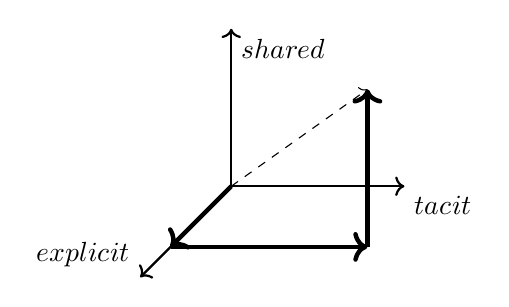
\begin{tikzpicture}
  \draw[thick,->] (0,0,0) -- (2.2,0,0) node[anchor= north west]{$tacit$};
  \draw[thick,->] (0,0,0) -- (0,2,0) node[anchor= north west]{$shared$};
  \draw[thick,->] (0,0,0) -- (0,0,3) node[anchor= south east]{$explicit$};

  \draw[ultra thick,->](0,0,0) -- (0,0,2);
  \draw[ultra thick,->](0,0,2) -- (2.5,0,2);
  \draw[ultra thick,->](2.5,0,2) -- (2.5, 2,2);
  \draw[dashed,->](0, 0, 0) -- (2.5, 2, 2);
\end{tikzpicture}

\begin{enumerate}
\def\labelenumi{(\arabic{enumi})}
\setcounter{enumi}{15}
\tightlist
\item
  Dimensions of knowledge
\end{enumerate}

\begin{center}\rule{0.5\linewidth}{0.5pt}\end{center}

In figure 16, one can see a path to knowledge. Around the year 1418,
Prince Henry the Navigator founded a School of Navigation in Sagres. In
the classroom, a future sailor was trained in map-making and reading,
which is explicit knowledge that one can write in books. The student
would advance along the explicit axis, as shown in figure 16. Then he
would embark on a vessel, where he would acquire actual job skills
through hands-on training. Could a sailor learn about maps while already
on a ship? Such a training method is represented by the dotted path in
figure 16 and is very dangerous. It is like a physician who would
consult the Sobotta to learn Anatomy while performing surgery.

One acquires tacit knowledge through training, there is no other way.
Don't expect to learn how to play the violin, become a wrestler, deliver
babies or pilot a jet plane exclusively from a classroom setting or from
books and youtube videos.

The shared knowledge is the one that cannot be found between our two
ears. It is distributed throughout organizations or expert guilds. For
instance, the knowledge about air combat, on which Manfred von
Richthofen -- the Red Baron -- excelled, was distributed between the
pilot, who was the Baron himself, and Anthony Fokker, the Dutch engineer
that designed Manfred's triplane. This knowledge was seamed so well that
the Baron could not perceive the stitches. The Red Baron was not able to
note the gaps in his dominance of the airplane, even when those gaps
were filled by automatic contrivances hard wired into the controls by
Anthony Fokker. In fact, any perceptible transition between engineering
expertise and flight tacit knowledge could hinder the pilot's ability to
anticipate the consequences of his actions and be fatal in a battle.

I am telling you all this in a attempt to convince you that this book
alone will not take you very far from the axis of explicit knowledge.

\chapter{Variations on a theme of
Vindaar}\label{variations-on-a-theme-of-vindaar}

\begin{Shaded}
\begin{Highlighting}[]
\CommentTok{\# counter.nim}
\KeywordTok{import}\NormalTok{ macros}\KeywordTok{,}\NormalTok{ strutils}\KeywordTok{,}\NormalTok{ os}

\KeywordTok{proc }\StringTok{parseArgs}\KeywordTok{(}\NormalTok{cmd}\KeywordTok{:} \DataTypeTok{NimNode}\KeywordTok{):} \KeywordTok{(}\DataTypeTok{NimNode}\KeywordTok{,} \DataTypeTok{NimNode}\KeywordTok{)} \CommentTok{=}
  \DataTypeTok{doAssert}\NormalTok{ cmd}\KeywordTok{.}\DataTypeTok{len} \CommentTok{==} \DecValTok{2}
  \DataTypeTok{expectKind}\KeywordTok{(}\NormalTok{cmd}\KeywordTok{[}\DecValTok{0}\KeywordTok{],}\NormalTok{ nnkIdent}\KeywordTok{)}
  \OtherTok{result} \CommentTok{=} \KeywordTok{(}\DataTypeTok{cmd}\KeywordTok{[}\DecValTok{0}\KeywordTok{],} \CommentTok{\# cmd[0] has an integer expr}
\NormalTok{            cmd}\KeywordTok{[}\DecValTok{1}\KeywordTok{])} \CommentTok{\# identifier to use for loop}

\KeywordTok{macro }\StringTok{cnt}\KeywordTok{(}\NormalTok{cmd}\KeywordTok{:} \DataTypeTok{untyped}\KeywordTok{,}\NormalTok{ stmts}\KeywordTok{:} \DataTypeTok{untyped}\KeywordTok{):} \DataTypeTok{untyped} \CommentTok{=}
  \DataTypeTok{expectKind}\KeywordTok{(}\NormalTok{cmd}\KeywordTok{,}\NormalTok{ nnkCommand}\KeywordTok{)}
  \DataTypeTok{expectKind}\KeywordTok{(}\NormalTok{stmts}\KeywordTok{,}\NormalTok{ nnkStmtList}\KeywordTok{)}
  \KeywordTok{let} \KeywordTok{(}\NormalTok{iterVar}\KeywordTok{,}\NormalTok{ toIdx}\KeywordTok{)} \CommentTok{=} \DataTypeTok{parseArgs}\KeywordTok{(}\NormalTok{cmd}\KeywordTok{)}
  \OtherTok{result} \CommentTok{=} \DataTypeTok{quote} \DataTypeTok{do}\KeywordTok{:}
    \DataTypeTok{for}\NormalTok{ \textasciigrave{}iterVar\textasciigrave{} }\CommentTok{in} \DecValTok{1}\KeywordTok{..}\NormalTok{\textasciigrave{}toIdx\textasciigrave{}}\KeywordTok{:}
\NormalTok{      \textasciigrave{}stmts\textasciigrave{}}
  \DataTypeTok{echo} \OtherTok{result}\KeywordTok{.}\DataTypeTok{repr}

\DataTypeTok{cnt} \DataTypeTok{j} \DataTypeTok{paramStr}\KeywordTok{(}\DecValTok{1}\KeywordTok{).}\DataTypeTok{parseInt}\KeywordTok{:}
    \DataTypeTok{echo}\NormalTok{ j}\KeywordTok{,} \StringTok{"{-} Give me some beer"}

\CommentTok{\#[ › ./build.nim scounter}
\CommentTok{   nim c {-}o:counter.x {-}d:danger {-}{-}hints:off {-}{-}nimcache:lixo counter.nim}
\CommentTok{   for j in 1 .. paramStr(1).parseInt:}
\CommentTok{       echo j, "{-} Give me some beer"}
\CommentTok{   › bin/counter.x 2}
\CommentTok{   1{-} Give me some beer}
\CommentTok{   2{-} Give me some beer}
\CommentTok{]\#}
\end{Highlighting}
\end{Shaded}

\begin{enumerate}
\def\labelenumi{(\arabic{enumi})}
\setcounter{enumi}{16}
\tightlist
\item
  A simpler counting macro
\end{enumerate}

When Vindaar provided us with the macro on listing 15, he gave us
explicit knowledge. In fact, since he could present the macro on paper,
it was explicit knowledge. In order to learn macro design, it is
necessary to practice, and one should start practicing with simple
stuff. In listing 17, the definition of \texttt{cnt} couldn't be
simpler. The \texttt{cmd} parameter has 2 elements, the first one must
be a variable. The statements below check whether these two conditions
are met by the \texttt{cnt} macro.

\begin{verbatim}
  doAssert cmd.len == 2
  expectKind(cmd[0], nnkIdent)
\end{verbatim}

\chapter{More Variations}\label{more-variations}

\begin{Shaded}
\begin{Highlighting}[]
\CommentTok{\# infixLoop.nim}
\KeywordTok{import}\NormalTok{ macros}\KeywordTok{,}\NormalTok{ strutils}\KeywordTok{,}\NormalTok{ os}

\KeywordTok{proc }\StringTok{parseArgs}\KeywordTok{(}\NormalTok{cmd}\KeywordTok{:} \DataTypeTok{NimNode}\KeywordTok{):} \KeywordTok{(}\DataTypeTok{NimNode}\KeywordTok{,} \DataTypeTok{NimNode}\KeywordTok{)} \CommentTok{=}
  \DataTypeTok{expectKind}\KeywordTok{(}\NormalTok{cmd}\KeywordTok{[}\DecValTok{0}\KeywordTok{],}\NormalTok{ nnkIdent}\KeywordTok{)}
  \DataTypeTok{expectKind}\KeywordTok{(}\NormalTok{cmd}\KeywordTok{[}\DecValTok{1}\KeywordTok{],}\NormalTok{ nnkIdent}\KeywordTok{)}
  \DataTypeTok{doAssert}\NormalTok{ cmd}\KeywordTok{[}\DecValTok{0}\KeywordTok{].}\DataTypeTok{strVal} \CommentTok{==} \StringTok{"++="}
  \OtherTok{result} \CommentTok{=} \KeywordTok{(}\NormalTok{cmd}\KeywordTok{[}\DecValTok{1}\KeywordTok{],}\NormalTok{ cmd}\KeywordTok{[}\DecValTok{2}\KeywordTok{])} 

\KeywordTok{macro }\StringTok{rpt}\KeywordTok{(}\NormalTok{cmd}\KeywordTok{:} \DataTypeTok{untyped}\KeywordTok{,}\NormalTok{ stmts}\KeywordTok{:} \DataTypeTok{untyped}\KeywordTok{):} \DataTypeTok{untyped} \CommentTok{=}
  \DataTypeTok{expectKind}\KeywordTok{(}\NormalTok{cmd}\KeywordTok{,}\NormalTok{ nnkInfix}\KeywordTok{)}
  \DataTypeTok{expectKind}\KeywordTok{(}\NormalTok{stmts}\KeywordTok{,}\NormalTok{ nnkStmtList}\KeywordTok{)}
  \KeywordTok{let} \KeywordTok{(}\NormalTok{iterVar}\KeywordTok{,}\NormalTok{ toIdx}\KeywordTok{)} \CommentTok{=} \DataTypeTok{parseArgs}\KeywordTok{(}\NormalTok{cmd}\KeywordTok{)}
  \OtherTok{result} \CommentTok{=} \DataTypeTok{quote} \DataTypeTok{do}\KeywordTok{:}
    \DataTypeTok{for}\NormalTok{ \textasciigrave{}iterVar\textasciigrave{} }\CommentTok{in} \DecValTok{1}\KeywordTok{..}\NormalTok{\textasciigrave{}toIdx\textasciigrave{}}\KeywordTok{:}
\NormalTok{      \textasciigrave{}stmts\textasciigrave{}}

\DataTypeTok{rpt}\NormalTok{ j }\CommentTok{++=} \DataTypeTok{paramStr}\KeywordTok{(}\DecValTok{1}\KeywordTok{).}\DataTypeTok{parseInt}\KeywordTok{:}
    \DataTypeTok{echo}\NormalTok{ j}\KeywordTok{,} \StringTok{"{-} Give me some beer"}

\CommentTok{\#[}
\CommentTok{› nim c {-}o:infixLoop.x {-}d:danger {-}{-}hints:off infixLoop.nim}

\CommentTok{› ./infixLoop.x 3}
\CommentTok{1{-} Give me some beer}
\CommentTok{2{-} Give me some beer}
\CommentTok{3{-} Give me some beer}
\CommentTok{]\#}
\end{Highlighting}
\end{Shaded}

\begin{enumerate}
\def\labelenumi{(\arabic{enumi})}
\setcounter{enumi}{17}
\tightlist
\item
  Macro with an infix operator
\end{enumerate}

Listing 18 is my second attempt at building an interesting macro. This
time, \texttt{cmd} has a single infix expression. I learned that I
should not place an assertion on the length of infix expressions. For
instance, the compiler protests if I add the following check on the
definition of \texttt{parseArgs} in listing 18:

\begin{verbatim}
proc parseArgs(cmd: NimNode): (NimNode, NimNode) =
  doAssert cmd.len == 2
  expectKind(cmd[0], nnkIdent)
  expectKind(cmd[1], nnkIdent)
  doAssert cmd[0].strVal == "++="
  result = (cmd[1], cmd[2]) 
\end{verbatim}

It seems that infix expressions do not have length. I would never
discover this if I had not been practicing over the last three days.

\chapter{Tree constructors}\label{tree-constructors}

\begin{Shaded}
\begin{Highlighting}[]
\CommentTok{\# ./build.nims akavelIter}
\KeywordTok{import}\NormalTok{ macros}\KeywordTok{,}\NormalTok{ strutils}\KeywordTok{,}\NormalTok{ os}

\KeywordTok{macro }\StringTok{iter}\KeywordTok{(}\NormalTok{cmd}\KeywordTok{:} \DataTypeTok{untyped}\KeywordTok{,}\NormalTok{ stmts}\KeywordTok{:} \DataTypeTok{untyped}\KeywordTok{):} \DataTypeTok{untyped} \CommentTok{=}
  \DataTypeTok{expectKind}\KeywordTok{(}\NormalTok{cmd}\KeywordTok{,}\NormalTok{ nnkInfix}\KeywordTok{)}
  \DataTypeTok{expectKind}\KeywordTok{(}\NormalTok{cmd}\KeywordTok{[}\DecValTok{0}\KeywordTok{],}\NormalTok{ nnKIdent}\KeywordTok{)}
  \DataTypeTok{doAssert}\NormalTok{ cmd}\KeywordTok{[}\DecValTok{0}\KeywordTok{].}\DataTypeTok{strVal} \CommentTok{==} \StringTok{"{-}\textgreater{}"}
  \DataTypeTok{expectKind}\KeywordTok{(}\NormalTok{cmd}\KeywordTok{[}\DecValTok{2}\KeywordTok{],}\NormalTok{ nnkIdent}\KeywordTok{)}
  \DataTypeTok{expectKind}\KeywordTok{(}\NormalTok{stmts}\KeywordTok{,}\NormalTok{ nnkStmtList}\KeywordTok{)}
  \KeywordTok{let} \KeywordTok{(}\NormalTok{ix}\KeywordTok{,}\NormalTok{ rng}\KeywordTok{)} \CommentTok{=} \KeywordTok{(}\NormalTok{cmd}\KeywordTok{[}\DecValTok{2}\KeywordTok{],}\NormalTok{ cmd}\KeywordTok{[}\DecValTok{1}\KeywordTok{])}
  \OtherTok{result} \CommentTok{=}\NormalTok{ nnkStmtList}\KeywordTok{.}\DataTypeTok{newTree}\KeywordTok{(}\NormalTok{nnkForStmt}\KeywordTok{.}\DataTypeTok{newTree}\KeywordTok{(}\NormalTok{ix}\KeywordTok{,}\NormalTok{ rng}\KeywordTok{,}\NormalTok{ stmts}\KeywordTok{))}

\DataTypeTok{iter} \DecValTok{3}\KeywordTok{..}\DataTypeTok{paramStr}\KeywordTok{(}\DecValTok{1}\KeywordTok{).}\DataTypeTok{parseInt} \CommentTok{{-}\textgreater{}}\NormalTok{ j}\KeywordTok{:}
    \DataTypeTok{echo}\NormalTok{ j}\KeywordTok{,} \StringTok{"{-} Give me some beer"}
\end{Highlighting}
\end{Shaded}

\begin{enumerate}
\def\labelenumi{(\arabic{enumi})}
\setcounter{enumi}{18}
\tightlist
\item
  An iterating program by akavel
\end{enumerate}

Here is an example of running iter:

\begin{verbatim}
~/nim/nimacros/src master ×
› ./build.nims akavelIter
nim c -o:akavelIter.x -d:danger --hints:off akavelIter.nim

~/nim/nimacros/src master ×
› bin/akavelIter.x 5
3- Give me some beer
4- Give me some beer
5- Give me some beer
\end{verbatim}

Program 19 shows that different people choose different solutions to the
same problem. The programmer whose nickname is \emph{vindaar} used a
quote pattern for creating the Abstract Syntactic Tree of a loop.

Another programmer, whose nickname is \emph{akavel}, I believe his true
name is Mateusz Czapliński, prefers to use the tree constructor
directly.

Languages such as Lisp and Scheme use the same kind of node for any
tree, the \texttt{consp} data structure, therefore, Lisp and Scheme need
only a tree constructor, to wit, the \texttt{cons} function. In an
Abstract Syntactic Tree, when it is necessary to differentiate one node
from the other, a Lisp programmer will put the identifier as the first
element in the list of ramifications. This is an elegant solution that
makes Lisp terse and powerful.

The design of Nim opted by using different nodes. Consider the program
of listing 19. The node that represents the statement list,
\texttt{nnkStmtList}, is completely different from the
\texttt{nnkForStmt} node, which represents the \texttt{for-loop}. The
Nim approach to AST construction has the advantage of preventing a kind
of error that is very common in Lisp, which is inserting a wrong node
identifier in the tree. However, the Nim system has also a serious
drawback, which is memorizing a different node constructing method for
each kind of node.

In listing 20 below, you will find a variation of the \texttt{iter}
loop. As far as I understand, a Nim command has two components, the part
that comes before the colon, and the part that comes after the colon.
The difference between listings 19 and 20 is restricted to the syntax of
the part that comes before the colon.

\begin{verbatim}
# ./build.nims akavelLoop
import macros, strutils, os

macro iter(cmd: untyped, sts: untyped): untyped =
  # Checking syntax of command
  expectKind(cmd, nnkCommand)
  doAssert cmd.len == 2
  expectKind(cmd[1], nnkInfix)
  for i in 0..2: expectKind(cmd[1][i], nnkIdent)
  doAssert cmd[1][0].strVal == "->"
  doAssert cmd[1][1].strVal == "times"
  expectKind(sts, nnkStmtList)
  let
    rng = cmd[0]
    ix = cmd[1][2]
  result = nnkStmtList.newTree(nnkForStmt.newTree(ix, rng, sts))

iter (3..paramStr(1).parseInt) times -> j:
    echo j, "- Give me some beer"
    echo "Now"
\end{verbatim}

\begin{enumerate}
\def\labelenumi{(\arabic{enumi})}
\setcounter{enumi}{19}
\tightlist
\item
  A more elaborate syntax for \texttt{iter}
\end{enumerate}

\chapter{A Lisp-like macro toolkit}\label{a-lisp-like-macro-toolkit}

\label{chp:Lisp-like-macro}

\begin{Shaded}
\begin{Highlighting}[]
\CommentTok{\# nim c {-}o:cons.x {-}d:danger {-}{-}hints:off {-}{-}nimcache:xx lispmacros.nim }
\KeywordTok{import}\NormalTok{ os}\KeywordTok{,}\NormalTok{ strutils}\KeywordTok{,}\NormalTok{ macros}\KeywordTok{,}\NormalTok{ consp}

\KeywordTok{macro }\StringTok{def}\KeywordTok{(}\NormalTok{id}\KeywordTok{:}\DataTypeTok{untyped}\KeywordTok{,}\NormalTok{ x}\KeywordTok{:}\DataTypeTok{untyped}\KeywordTok{,}\NormalTok{ y}\KeywordTok{:}\DataTypeTok{untyped}\KeywordTok{):} \DataTypeTok{untyped}\CommentTok{=}
  \KeywordTok{let}\NormalTok{ ix}\CommentTok{=}\NormalTok{ x}\KeywordTok{.}\DataTypeTok{strVal}\KeywordTok{.}\DataTypeTok{sy}
  \KeywordTok{let}\NormalTok{ iy}\CommentTok{=}\NormalTok{ y}\KeywordTok{.}\DataTypeTok{strVal}\KeywordTok{.}\DataTypeTok{sy}
  \KeywordTok{let}\NormalTok{ body}\CommentTok{=} \DataTypeTok{cons}\KeywordTok{(}\NormalTok{plus}\KeywordTok{,} \DataTypeTok{cons}\KeywordTok{(}\NormalTok{ix}\KeywordTok{,} \DataTypeTok{cons}\KeywordTok{(}\NormalTok{iy}\KeywordTok{,} \FloatTok{nil}\KeywordTok{))).}\DataTypeTok{walkAST}
  \DataTypeTok{quote} \DataTypeTok{do}\KeywordTok{:}
    \KeywordTok{proc }\StringTok{\textasciigrave{}id\textasciigrave{}}\KeywordTok{(}\NormalTok{\textasciigrave{}x\textasciigrave{}}\KeywordTok{:} \DataTypeTok{int}\KeywordTok{,}\NormalTok{ \textasciigrave{}y\textasciigrave{}}\KeywordTok{:} \DataTypeTok{int}\KeywordTok{):} \DataTypeTok{int}\CommentTok{=}
\NormalTok{       \textasciigrave{}body\textasciigrave{}}

\DataTypeTok{def}\KeywordTok{(}\NormalTok{sum}\KeywordTok{,}\NormalTok{ cx}\KeywordTok{,}\NormalTok{ cy}\KeywordTok{)}

\DataTypeTok{echo} \DataTypeTok{cons}\KeywordTok{(}\StringTok{"hi"}\KeywordTok{.}\DataTypeTok{sy}\KeywordTok{,} \DataTypeTok{cons}\KeywordTok{(}\DecValTok{42}\KeywordTok{.}\DataTypeTok{mI}\KeywordTok{,} \DataTypeTok{cons}\KeywordTok{(}\DataTypeTok{cons}\KeywordTok{(}\StringTok{"world"}\KeywordTok{.}\DataTypeTok{sy}\KeywordTok{,} \FloatTok{nil}\KeywordTok{),} \FloatTok{nil}\KeywordTok{)))}
\DataTypeTok{echo} \DataTypeTok{sum}\KeywordTok{(}\DataTypeTok{paramStr}\KeywordTok{(}\DecValTok{1}\KeywordTok{).}\DataTypeTok{parseInt}\KeywordTok{,} \DecValTok{8}\KeywordTok{)}
 
\end{Highlighting}
\end{Shaded}

\begin{enumerate}
\def\labelenumi{(\arabic{enumi})}
\setcounter{enumi}{20}
\tightlist
\item
  A Lisp style macro
\end{enumerate}

Here is an example of the above program in action:

\begin{verbatim}
› nim c -o:cons.x -d:danger --hints:off --nimcache:xx lispmacros.nim
› ./cons.x 34
(hi 42 (world))
42
\end{verbatim}

In Lisp, it is customary to represent any kind of tree as a combination
of binary trees. The great advantage of this approach is that Lisp
programmers need to learn only one constructor of branches, the
\texttt{cons} node. In a future version of this tutorial, I intend to
give a lengthy introduction to the Lisp method of dealing with tree. One
last thing, in order to compile the program of listing 21, you need to
keep the library of listing 22 in the same folder.

\pagebreak

\begin{Shaded}
\begin{Highlighting}[]
\CommentTok{\# Library: consp.nim}
\KeywordTok{import}\NormalTok{ strutils}\KeywordTok{,}\NormalTok{ macros}
\KeywordTok{type}
  \DataTypeTok{SExprKind} \CommentTok{=} \KeywordTok{enum }\DataTypeTok{Intp}\KeywordTok{,} \DataTypeTok{Floatp}\KeywordTok{,} \DataTypeTok{St}\KeywordTok{,} \DataTypeTok{Sym}\KeywordTok{,}\NormalTok{ consp}
  \DataTypeTok{SExpr} \CommentTok{=} \DataTypeTok{ref} \KeywordTok{object}
       \DataTypeTok{case}\NormalTok{ kind}\KeywordTok{:} \DataTypeTok{SExprKind}
       \CommentTok{of} \DataTypeTok{Intp}\KeywordTok{:}\NormalTok{ intVal}\KeywordTok{:} \DataTypeTok{int}
       \CommentTok{of} \DataTypeTok{Floatp}\KeywordTok{:}\NormalTok{ floatVal}\KeywordTok{:} \DataTypeTok{float}
       \CommentTok{of} \DataTypeTok{Sym}\KeywordTok{:}\NormalTok{ symb}\KeywordTok{:} \DataTypeTok{string}
       \CommentTok{of} \DataTypeTok{St}\KeywordTok{:}\NormalTok{ str}\KeywordTok{:} \DataTypeTok{string}
       \CommentTok{of}\NormalTok{ consp}\KeywordTok{:}\NormalTok{ h}\KeywordTok{,}\NormalTok{ t}\KeywordTok{:} \DataTypeTok{SExpr}

\KeywordTok{template }\StringTok{mI}\CommentTok{*}\KeywordTok{(}\NormalTok{a}\KeywordTok{:}\DataTypeTok{int}\KeywordTok{):} \DataTypeTok{SExpr}\CommentTok{=} \DataTypeTok{SExpr}\KeywordTok{(}\NormalTok{kind}\KeywordTok{:} \DataTypeTok{Intp}\KeywordTok{,}\NormalTok{ intVal}\KeywordTok{:}\NormalTok{ a}\KeywordTok{)}
\KeywordTok{template }\StringTok{sy}\CommentTok{*}\KeywordTok{(}\NormalTok{s}\KeywordTok{:} \DataTypeTok{string}\KeywordTok{):} \DataTypeTok{SExpr}\CommentTok{=} \DataTypeTok{SExpr}\KeywordTok{(}\NormalTok{kind}\KeywordTok{:} \DataTypeTok{Sym}\KeywordTok{,}\NormalTok{ symb}\KeywordTok{:}\NormalTok{ \textasciigrave{}s\textasciigrave{}}\KeywordTok{)}
\KeywordTok{template }\StringTok{car}\CommentTok{*}\KeywordTok{(}\NormalTok{s}\KeywordTok{:}\DataTypeTok{SExpr}\KeywordTok{):} \DataTypeTok{SExpr}\CommentTok{=}\NormalTok{ s}\KeywordTok{.}\DataTypeTok{h}
\KeywordTok{template }\StringTok{cdr}\CommentTok{*}\KeywordTok{(}\NormalTok{s}\KeywordTok{:}\DataTypeTok{SExpr}\KeywordTok{):} \DataTypeTok{Sexpr}\CommentTok{=}\NormalTok{ s}\KeywordTok{.}\DataTypeTok{t}
\KeywordTok{template }\StringTok{cons}\CommentTok{*}\KeywordTok{(}\NormalTok{x}\KeywordTok{:}\DataTypeTok{SExpr}\KeywordTok{,}\NormalTok{ y}\KeywordTok{:}\DataTypeTok{SExpr}\KeywordTok{):} \DataTypeTok{SExpr}\CommentTok{=} \DataTypeTok{SExpr}\KeywordTok{(}\NormalTok{kind}\KeywordTok{:}\NormalTok{ consp}\KeywordTok{,}\NormalTok{ h}\KeywordTok{:}\NormalTok{ x}\KeywordTok{,}\NormalTok{ t}\KeywordTok{:}\NormalTok{ y}\KeywordTok{)}

\KeywordTok{proc }\StringTok{\textasciigrave{}$\textasciigrave{}}\CommentTok{*}\KeywordTok{(}\NormalTok{se}\KeywordTok{:} \DataTypeTok{SExpr}\KeywordTok{):} \DataTypeTok{string} \CommentTok{=}
  \DataTypeTok{case}\NormalTok{ se}\KeywordTok{.}\DataTypeTok{kind}
  \CommentTok{of} \DataTypeTok{Intp}\KeywordTok{:} \OtherTok{result}\CommentTok{=} \CommentTok{$}\NormalTok{se}\KeywordTok{.}\DataTypeTok{intVal}
  \CommentTok{of} \DataTypeTok{Floatp}\KeywordTok{:} \OtherTok{result} \CommentTok{=} \CommentTok{$}\NormalTok{se}\KeywordTok{.}\DataTypeTok{floatVal}
  \CommentTok{of} \DataTypeTok{ST}\KeywordTok{:} \OtherTok{result} \CommentTok{=} \CharTok{\textquotesingle{}"\textquotesingle{}} \CommentTok{\&}\NormalTok{ se}\KeywordTok{.}\DataTypeTok{str} \CommentTok{\&} \CharTok{\textquotesingle{}"\textquotesingle{}}
  \CommentTok{of} \DataTypeTok{Sym}\KeywordTok{:} \OtherTok{result} \CommentTok{=}\NormalTok{ se}\KeywordTok{.}\DataTypeTok{symb}
  \CommentTok{of}\NormalTok{ consp}\KeywordTok{:}
    \OtherTok{result}\KeywordTok{.}\DataTypeTok{add}\KeywordTok{(}\StringTok{"("}\KeywordTok{)}
    \KeywordTok{var} \KeywordTok{(}\NormalTok{r}\KeywordTok{,}\NormalTok{ ind}\KeywordTok{)} \CommentTok{=} \KeywordTok{(}\NormalTok{se}\KeywordTok{,} \DecValTok{0}\KeywordTok{)}
    \DataTypeTok{while}\NormalTok{ r }\CommentTok{!=} \FloatTok{nil}\KeywordTok{:}
      \OtherTok{result}\KeywordTok{.}\DataTypeTok{add}\KeywordTok{(}\DataTypeTok{indent}\KeywordTok{(}\CommentTok{$}\NormalTok{r}\KeywordTok{.}\DataTypeTok{car}\KeywordTok{,}\NormalTok{ ind}\KeywordTok{))}
      \KeywordTok{(}\NormalTok{r}\KeywordTok{,}\NormalTok{ ind}\KeywordTok{)}\CommentTok{=} \KeywordTok{(}\NormalTok{r}\KeywordTok{.}\DataTypeTok{cdr}\KeywordTok{,} \DecValTok{1}\KeywordTok{)}
    \OtherTok{result}\KeywordTok{.}\DataTypeTok{add}\KeywordTok{(}\StringTok{")"}\KeywordTok{)}

\KeywordTok{let}\NormalTok{ plus}\CommentTok{*}\AttributeTok{\{.compileTime.\}}\CommentTok{=}  \StringTok{"+"}\KeywordTok{.}\DataTypeTok{sy}
\KeywordTok{proc }\StringTok{walkAST}\CommentTok{*}\KeywordTok{(}\NormalTok{e}\KeywordTok{:}\DataTypeTok{SExpr}\KeywordTok{):} \DataTypeTok{NimNode} \CommentTok{=}
   \DataTypeTok{case}\NormalTok{ e}\KeywordTok{.}\DataTypeTok{kind}\KeywordTok{:}
     \CommentTok{of} \DataTypeTok{Sym}\KeywordTok{:} \DataTypeTok{return} \DataTypeTok{newIdentNode}\NormalTok{ e}\KeywordTok{.}\DataTypeTok{symb}
     \CommentTok{of} \DataTypeTok{Intp}\KeywordTok{:} \DataTypeTok{return} \DataTypeTok{newLit}\NormalTok{ e}\KeywordTok{.}\DataTypeTok{intVal}
     \CommentTok{of}\NormalTok{ consp}\KeywordTok{:}
       \DataTypeTok{if} \DataTypeTok{car}\KeywordTok{(}\NormalTok{e}\KeywordTok{)} \CommentTok{==}\NormalTok{ plus}\KeywordTok{:}
         \DataTypeTok{return}\NormalTok{ nnkCall}\KeywordTok{.}\DataTypeTok{newTree}\KeywordTok{(}\NormalTok{ newIdentNode}\StringTok{"+"}\KeywordTok{,}
\NormalTok{                                 e}\KeywordTok{.}\DataTypeTok{cdr}\KeywordTok{.}\DataTypeTok{car}\KeywordTok{.}\DataTypeTok{walkAST}\KeywordTok{,}
\NormalTok{                                 e}\KeywordTok{.}\DataTypeTok{cdr}\KeywordTok{.}\DataTypeTok{cdr}\KeywordTok{.}\DataTypeTok{car}\KeywordTok{.}\DataTypeTok{walkAST}\KeywordTok{)}
     \DataTypeTok{else}\KeywordTok{:} \DataTypeTok{return} \DataTypeTok{newLit} \StringTok{"Erro"}
\end{Highlighting}
\end{Shaded}

\begin{enumerate}
\def\labelenumi{(\arabic{enumi})}
\setcounter{enumi}{21}
\tightlist
\item
  A Library for the \texttt{consp} data structure
\end{enumerate}

\chapter{Finite Automaton}\label{finite-automaton}

\begin{figure}[!h]
\renewcommand\figurename{Fig.}
\begin{tikzpicture}[shorten >=1pt,
                   auto,node distance=3cm]
\node[initial,state,accepting] (S)      {$S$};
\node[state]         (q0) [right of=S]  {$skp$};
\node[state]         (q1) [right of=q0]  {$q_1$};
\node[state]         (q3) [right of=q1] {$q_2$};
\node[state]         (r0) [below of= S] {$\rightarrow n$};
\node[state]         (q2) [below of=q1] {$\rightarrow n$};

\path[->] (S)  edge  (q0)
(q0) edge [->] node {\small else} (q1)
(q1) edge [bend right] node {.,:?!} (q2)
(q0) edge [loop above] node {blank} (q0)
(q3) edge [bend left=60] node {\small else} (q2)
(q1) edge [->,bend left] node {else} (q3)
(q1) edge [] node {""} (r0);
\path[->]
(q3) edge [loop right] node {a-z} (q3);
\end{tikzpicture}
\caption{Finite automaton that recognizes English words}
\label{fig:automaton}
\end{figure}

A deterministic finite automaton is a finite state machine that accepts
or rejects finite strings of chars and only produces a unique
computation for each input string. Figure \ref{fig:automaton} above
illustrates a deterministic finite automaton using a state diagram. The
aforementioned automaton recognizes words and puctuation marks from a
text using the Roman alphabet, which is the same as in English.
Therefore, this automaton can accept a stream of words and punctuation
from an English text.

In the automaton of figure \ref{fig:automaton}, there are three states:
\(skp\), \(q_1\) and \(q_2\). The automaton remains in the state
\(skp\), while the stream produces blank chars, i.e., \verb|' '|,
\texttt{newline} or \texttt{TAB}. If the computation reaches the end of
the string, the automaton stops. If a punctuation mark appears in the
stream, the automaton accepts it, and returns \(\rightarrow n\). If the
\(q_1\) state receives an alphabetical letter, the automaton goes to
state \(q_2\) and remains there, while the reader keeps feeding letters.

The program of listing 23 implements the finite automaton and stores the
tokens into a singly linked list, of the same sort that you learned in
chapter \ref{chp:Lisp-like-macro}. I hope that by now you will be able
to compile and test the program without the need for detailed
instruction.

\begin{Shaded}
\begin{Highlighting}[]
\KeywordTok{type}
   \DataTypeTok{LLKind} \CommentTok{=} \KeywordTok{enum }\DataTypeTok{Sym}\KeywordTok{,}\NormalTok{ consp}
   \DataTypeTok{LL}\CommentTok{=} \DataTypeTok{ref} \KeywordTok{object }\DataTypeTok{of}\CommentTok{ }\DataTypeTok{RootObj}
     \DataTypeTok{case}\NormalTok{ kind}\KeywordTok{:} \DataTypeTok{LLKind}
     \CommentTok{of} \DataTypeTok{Sym}\KeywordTok{:}\NormalTok{ symb}\KeywordTok{:} \DataTypeTok{string}
     \CommentTok{of}\NormalTok{ consp}\KeywordTok{:}\NormalTok{ car}\KeywordTok{,}\NormalTok{ cdr}\KeywordTok{:} \DataTypeTok{LL}

\KeywordTok{template }\StringTok{sy}\CommentTok{*}\KeywordTok{(}\NormalTok{s}\KeywordTok{:} \DataTypeTok{string}\KeywordTok{):}  \DataTypeTok{LL}\CommentTok{=} \DataTypeTok{LL}\KeywordTok{(}\NormalTok{kind}\KeywordTok{:} \DataTypeTok{Sym}\KeywordTok{,}\NormalTok{  symb}\KeywordTok{:}\NormalTok{ \textasciigrave{}s\textasciigrave{}}\KeywordTok{)}
\KeywordTok{template }\StringTok{\textasciigrave{}\textgreater{}\textgreater{}\textasciigrave{}}\CommentTok{ }\KeywordTok{(}\NormalTok{a}\KeywordTok{,}\NormalTok{b}\KeywordTok{:} \DataTypeTok{LL}\KeywordTok{):} \DataTypeTok{LL}\CommentTok{=} \DataTypeTok{LL}\KeywordTok{(}\NormalTok{kind}\KeywordTok{:}\NormalTok{ consp}\KeywordTok{,}\NormalTok{ car}\KeywordTok{:}\NormalTok{ a}\KeywordTok{,}\NormalTok{ cdr}\KeywordTok{:}\NormalTok{ b}\KeywordTok{)}

\KeywordTok{proc }\StringTok{tkz}\CommentTok{*}\KeywordTok{(}\NormalTok{s}\KeywordTok{:} \DataTypeTok{string}\KeywordTok{,}\NormalTok{  ix}\KeywordTok{:} \DataTypeTok{int}\KeywordTok{):} \DataTypeTok{LL} \CommentTok{=}
  \KeywordTok{proc }\StringTok{skp}\KeywordTok{(}\NormalTok{s}\KeywordTok{:} \DataTypeTok{string}\KeywordTok{,}\NormalTok{ i}\KeywordTok{:} \DataTypeTok{int}\KeywordTok{):} \DataTypeTok{int}\CommentTok{=}
    \DataTypeTok{if}\NormalTok{ i }\CommentTok{\textgreater{}=}\NormalTok{ s}\KeywordTok{.}\DataTypeTok{len}\KeywordTok{:} \OtherTok{result}\CommentTok{=}\NormalTok{ s}\KeywordTok{.}\DataTypeTok{len}
    \DataTypeTok{elif}\NormalTok{ s}\KeywordTok{[}\NormalTok{i}\KeywordTok{]} \CommentTok{==} \CharTok{\textquotesingle{} \textquotesingle{}} \KeywordTok{:} \OtherTok{result}\CommentTok{=} \DataTypeTok{skp}\KeywordTok{(}\NormalTok{s}\KeywordTok{,}\NormalTok{ i}\CommentTok{+}\DecValTok{1}\KeywordTok{)}
    \DataTypeTok{else}\KeywordTok{:} \OtherTok{result}\CommentTok{=}\NormalTok{ i}
  
  \KeywordTok{proc }\StringTok{q1}\KeywordTok{(}\NormalTok{s}\KeywordTok{:} \DataTypeTok{string}\KeywordTok{,}\NormalTok{ i}\KeywordTok{:} \DataTypeTok{int}\KeywordTok{):} \DataTypeTok{int}\CommentTok{=}
    \DataTypeTok{if}\NormalTok{ i }\CommentTok{\textgreater{}=}\NormalTok{ s}\KeywordTok{.}\DataTypeTok{len}\KeywordTok{:} \OtherTok{result}\CommentTok{=}\NormalTok{ i}\CommentTok{{-}}\DecValTok{1}
    \DataTypeTok{elif}\NormalTok{ s}\KeywordTok{[}\NormalTok{i}\KeywordTok{]} \CommentTok{in} \KeywordTok{\{}\CharTok{\textquotesingle{} \textquotesingle{}}\KeywordTok{,} \CharTok{\textquotesingle{},\textquotesingle{}}\KeywordTok{,} \CharTok{\textquotesingle{};\textquotesingle{}}\KeywordTok{,} \CharTok{\textquotesingle{}?\textquotesingle{}}\KeywordTok{\}:} \OtherTok{result}\CommentTok{=}\NormalTok{ i}\CommentTok{{-}}\DecValTok{1}
    \DataTypeTok{else}\KeywordTok{:} \OtherTok{result}\CommentTok{=} \DataTypeTok{q1}\KeywordTok{(}\NormalTok{s}\KeywordTok{,}\NormalTok{ i}\CommentTok{+}\DecValTok{1}\KeywordTok{)}
  
  \KeywordTok{var}\NormalTok{ i}\CommentTok{=} \DataTypeTok{skp}\KeywordTok{(}\NormalTok{s}\KeywordTok{,}\NormalTok{ ix}\KeywordTok{)}
  \DataTypeTok{if}\NormalTok{ i }\CommentTok{\textgreater{}=}\NormalTok{ s}\KeywordTok{.}\DataTypeTok{len}\KeywordTok{:} \DataTypeTok{return} \FloatTok{nil}
  \DataTypeTok{if}\NormalTok{ s}\KeywordTok{[}\NormalTok{i}\KeywordTok{]} \CommentTok{in} \KeywordTok{\{}\CharTok{\textquotesingle{},\textquotesingle{}}\KeywordTok{,} \CharTok{\textquotesingle{};\textquotesingle{}}\KeywordTok{,} \CharTok{\textquotesingle{}?\textquotesingle{}}\KeywordTok{\}:} \DataTypeTok{return}\NormalTok{ s}\KeywordTok{[}\NormalTok{i}\KeywordTok{..}\NormalTok{i}\KeywordTok{].}\DataTypeTok{sy} \CommentTok{\textgreater{}\textgreater{}} \DataTypeTok{tkz}\KeywordTok{(}\NormalTok{s}\KeywordTok{,}\NormalTok{ i}\CommentTok{+}\DecValTok{1}\KeywordTok{)}
  \KeywordTok{var}\NormalTok{ j}\CommentTok{=} \DataTypeTok{q1}\KeywordTok{(}\NormalTok{s}\KeywordTok{,}\NormalTok{ i}\KeywordTok{)}
  \DataTypeTok{if}\NormalTok{ j }\CommentTok{\textgreater{}=}\NormalTok{ s}\KeywordTok{.}\DataTypeTok{len}\KeywordTok{:} \DataTypeTok{return}\NormalTok{ s}\KeywordTok{[}\NormalTok{i}\KeywordTok{..}\NormalTok{s}\KeywordTok{.}\DataTypeTok{len}\CommentTok{{-}}\DecValTok{1}\KeywordTok{].}\DataTypeTok{sy} \CommentTok{\textgreater{}\textgreater{}} \FloatTok{nil}
  \DataTypeTok{else}\KeywordTok{:} \DataTypeTok{return}\NormalTok{ s}\KeywordTok{[}\NormalTok{i}\KeywordTok{..}\NormalTok{j}\KeywordTok{].}\DataTypeTok{sy} \CommentTok{\textgreater{}\textgreater{}} \DataTypeTok{tkz}\KeywordTok{(}\NormalTok{s}\KeywordTok{,}\NormalTok{ j}\CommentTok{+}\DecValTok{1}\KeywordTok{)}

\KeywordTok{proc }\StringTok{\textasciigrave{}$\textasciigrave{}}\CommentTok{*}\KeywordTok{(}\NormalTok{se}\KeywordTok{:} \DataTypeTok{LL}\KeywordTok{):} \DataTypeTok{string}\CommentTok{=}
 \DataTypeTok{case}\NormalTok{ se}\KeywordTok{.}\DataTypeTok{kind}
 \CommentTok{of} \DataTypeTok{Sym}\KeywordTok{:} \OtherTok{result} \CommentTok{=}\NormalTok{ se}\KeywordTok{.}\DataTypeTok{symb}
 \CommentTok{of}\NormalTok{ consp}\KeywordTok{:}
   \OtherTok{result}\KeywordTok{.}\DataTypeTok{add}\KeywordTok{(}\StringTok{"("}\KeywordTok{)}
   \KeywordTok{var} \KeywordTok{(}\NormalTok{r}\KeywordTok{,}\NormalTok{ ind}\KeywordTok{)} \CommentTok{=} \KeywordTok{(}\NormalTok{se}\KeywordTok{,} \StringTok{""}\KeywordTok{)}
   \DataTypeTok{while}\NormalTok{ r }\CommentTok{!=} \FloatTok{nil}\KeywordTok{:}
     \OtherTok{result}\KeywordTok{.}\DataTypeTok{add}\KeywordTok{(}\NormalTok{ind }\CommentTok{\&} \CommentTok{$}\NormalTok{r}\KeywordTok{.}\DataTypeTok{car}\KeywordTok{)}
     \KeywordTok{(}\NormalTok{r}\KeywordTok{,}\NormalTok{ ind}\KeywordTok{)}\CommentTok{=} \KeywordTok{(}\NormalTok{r}\KeywordTok{.}\DataTypeTok{cdr}\KeywordTok{,} \StringTok{" "}\KeywordTok{)}
   \OtherTok{result}\KeywordTok{.}\DataTypeTok{add}\KeywordTok{(}\StringTok{")"}\KeywordTok{)}

\DataTypeTok{echo} \DataTypeTok{tkz}\KeywordTok{(}\StringTok{"  She walks in beauty, like the night"}\KeywordTok{,}  \DecValTok{0}\KeywordTok{)} \CommentTok{\textgreater{}\textgreater{}}
         \KeywordTok{(}\DataTypeTok{tkz}\KeywordTok{(}\StringTok{"Of cloudless climes and starry skies;"}\KeywordTok{,} \DecValTok{0}\KeywordTok{)} \CommentTok{\textgreater{}\textgreater{}} \FloatTok{nil}\KeywordTok{)}
\end{Highlighting}
\end{Shaded}

\begin{enumerate}
\def\labelenumi{(\arabic{enumi})}
\setcounter{enumi}{22}
\tightlist
\item
  Finite Automaton in Nim
\end{enumerate}

\chapter{Nightmares}\label{nightmares}

I was born in Provo, a small town in Utah, about 82 miles from Salt Lake
City. If you are not acquainted with customary units, you will find a
good opportunity to practice Nim in the American units of measurement.
Therefore, let us interrupt my story and deal with unit conversions. Let
us consider only conversions between miles and kilometers for the time
being. You will discover easily how to deal with other units. Below, you
can see how to use the program of listing 24.

\begin{verbatim}
~/nim/tutorial/src
› ./build.nims units
nim c -o:units.x -d:danger --hints:off --nimcache:lixo units.nim

~/nim/tutorial/src
› bin/units.x
> 82 mi km
131.938km
> q
\end{verbatim}

As you are probably aware, there are a lot of Mormons in that region of
the United States. I myself am an atheist, as befits a physician. The
rest of my family are members of The Church of Jesus Christ of
Latter-day Saints, which is the official name of the Mormon Church.
Since The Church of Jesus Christ of Latter-day Saints is a very long
name to write or pronounce, Mormons often abbreviate it as The LDS
Church, an acronym that reminds me of a popular hallucinogenic drug.

A Mormon believes in many weird doctrines. According to the doctrine of
continuing revelation, Jesus Christ leads the LDS Church by revealing
his will to its president. The belief is also that each individual
member of the church can receive personal revelation from God, while
getting on with conducting his or her personal life. However, I never
did, which makes me the only Mormon to whom God never revealed anything!

Who is this guy that calls himself God? Apparently, he is a king that
rules the Earth from his throne somewhere near the star Kolob.

\pagebreak

\begin{Shaded}
\begin{Highlighting}[]
\CommentTok{\# ./build.nims units}
\KeywordTok{import}\NormalTok{ os}\KeywordTok{,}\NormalTok{ strutils}

\KeywordTok{type}
  \DataTypeTok{LL}\CommentTok{=} \DataTypeTok{ref} \KeywordTok{object }\DataTypeTok{of}\CommentTok{ }\DataTypeTok{RootObj}
\NormalTok{          h}\KeywordTok{:}  \DataTypeTok{U}
\NormalTok{          t}\KeywordTok{:} \DataTypeTok{LL}
  \DataTypeTok{UnitKind}\CommentTok{=} \KeywordTok{enum }\DataTypeTok{mi}\CommentTok{=} \StringTok{"mi"}\KeywordTok{,}\NormalTok{ km}\CommentTok{=} \StringTok{"km"}\KeywordTok{,}\NormalTok{ nm}\CommentTok{=} \StringTok{"nm"}
  \DataTypeTok{U} \CommentTok{=} \DataTypeTok{ref} \KeywordTok{object}
        \DataTypeTok{case}\NormalTok{ kind}\KeywordTok{:} \DataTypeTok{UnitKind}
           \CommentTok{of}\NormalTok{ mi}\KeywordTok{,}\NormalTok{ km}\KeywordTok{,}\NormalTok{ nm}\KeywordTok{:}\NormalTok{ fVal}\KeywordTok{:} \DataTypeTok{float}

\KeywordTok{template }\StringTok{car}\KeywordTok{(}\NormalTok{a}\KeywordTok{:}\DataTypeTok{untyped}\KeywordTok{)} \KeywordTok{:} \DataTypeTok{untyped}\CommentTok{=}
  \DataTypeTok{if}\NormalTok{ a }\CommentTok{==} \FloatTok{nil}\KeywordTok{:} \DataTypeTok{quit}\KeywordTok{(}\StringTok{"Empty stack"}\KeywordTok{)} \DataTypeTok{else}\KeywordTok{:}\NormalTok{ a}\KeywordTok{.}\DataTypeTok{h}

\KeywordTok{template }\StringTok{psh}\KeywordTok{(}\NormalTok{knd}\KeywordTok{:} \DataTypeTok{untyped}\KeywordTok{,}\NormalTok{ v}\KeywordTok{:} \DataTypeTok{untyped}\KeywordTok{,}\NormalTok{ s}\KeywordTok{:} \DataTypeTok{untyped}\KeywordTok{)} \CommentTok{=}
\NormalTok{  s }\CommentTok{=} \DataTypeTok{LL}\KeywordTok{(}\NormalTok{h}\KeywordTok{:} \DataTypeTok{U}\KeywordTok{(}\NormalTok{kind}\KeywordTok{:}\NormalTok{ knd}\KeywordTok{,}\NormalTok{ fVal}\KeywordTok{:}\NormalTok{ v}\KeywordTok{),}\NormalTok{ t}\KeywordTok{:}\NormalTok{ s}\KeywordTok{.}\DataTypeTok{t}\KeywordTok{)}

\KeywordTok{proc }\StringTok{eval}\KeywordTok{(}\NormalTok{x}\KeywordTok{:} \DataTypeTok{string}\KeywordTok{,}\NormalTok{ s}\KeywordTok{:} \KeywordTok{var} \DataTypeTok{LL}\KeywordTok{)}\CommentTok{=}
  \DataTypeTok{try}\KeywordTok{:}\NormalTok{ s}\CommentTok{=} \DataTypeTok{LL}\KeywordTok{(}\NormalTok{h}\KeywordTok{:} \DataTypeTok{U}\KeywordTok{(}\NormalTok{kind}\KeywordTok{:}\NormalTok{ nm}\KeywordTok{,}\NormalTok{ fVal}\KeywordTok{:}\NormalTok{ x}\KeywordTok{.}\DataTypeTok{strip}\KeywordTok{.}\DataTypeTok{parseFloat}\KeywordTok{),}\NormalTok{ t}\KeywordTok{:}\NormalTok{ s}\KeywordTok{)}
  \DataTypeTok{except}\KeywordTok{:}
    \DataTypeTok{case} \DataTypeTok{x} \KeywordTok{:}
      \CommentTok{of} \StringTok{"km"}\KeywordTok{:}
         \DataTypeTok{if} \KeywordTok{(}\DataTypeTok{car}\NormalTok{ s}\KeywordTok{).}\DataTypeTok{kind} \CommentTok{==}\NormalTok{ nm}\KeywordTok{:} \KeywordTok{(}\DataTypeTok{car}\NormalTok{ s}\KeywordTok{).}\DataTypeTok{kind}\CommentTok{=}\NormalTok{ km}
         \DataTypeTok{elif} \KeywordTok{(}\DataTypeTok{car}\NormalTok{ s}\KeywordTok{).}\DataTypeTok{kind} \CommentTok{==}\NormalTok{ mi}\KeywordTok{:} \DataTypeTok{psh}\KeywordTok{(}\NormalTok{km}\KeywordTok{,}\NormalTok{ s}\KeywordTok{.}\DataTypeTok{h}\KeywordTok{.}\DataTypeTok{fVal} \CommentTok{*} \DecValTok{1}\FloatTok{.}\DecValTok{609}\KeywordTok{,}\NormalTok{ s}\KeywordTok{)}
      \CommentTok{of} \StringTok{"mi"}\KeywordTok{:}
        \DataTypeTok{if} \KeywordTok{(}\DataTypeTok{car}\NormalTok{ s}\KeywordTok{).}\DataTypeTok{kind} \CommentTok{==}\NormalTok{ nm}\KeywordTok{:} \KeywordTok{(}\DataTypeTok{car}\NormalTok{ s}\KeywordTok{).}\DataTypeTok{kind}\CommentTok{=}\NormalTok{ mi}
        \DataTypeTok{elif} \KeywordTok{(}\DataTypeTok{car}\NormalTok{ s}\KeywordTok{).}\DataTypeTok{kind} \CommentTok{==}\NormalTok{ km}\KeywordTok{:} \DataTypeTok{psh}\KeywordTok{(}\NormalTok{mi}\KeywordTok{,}\NormalTok{ s}\KeywordTok{.}\DataTypeTok{h}\KeywordTok{.}\DataTypeTok{fVal} \CommentTok{/} \DecValTok{1}\FloatTok{.}\DecValTok{609}\KeywordTok{,}\NormalTok{ s}\KeywordTok{)}
      \DataTypeTok{else}\KeywordTok{:} \DataTypeTok{echo} \StringTok{"?"}

\KeywordTok{var}\NormalTok{ s}\CommentTok{=}  \StringTok{""}
\KeywordTok{var}\NormalTok{ stk}\KeywordTok{:} \DataTypeTok{LL}\CommentTok{=} \FloatTok{nil}
\KeywordTok{var}\NormalTok{ stack}\KeywordTok{:} \DataTypeTok{LL}\CommentTok{=} \FloatTok{nil}
\NormalTok{stdout}\KeywordTok{.}\DataTypeTok{write} \StringTok{"\textgreater{} "}
\DataTypeTok{while}\NormalTok{ stdin}\KeywordTok{.}\DataTypeTok{readline}\KeywordTok{(}\NormalTok{s}\KeywordTok{)} \CommentTok{and}\NormalTok{ s }\CommentTok{!=} \StringTok{"q"}\KeywordTok{:}
  \DataTypeTok{for}\NormalTok{ x }\CommentTok{in}\NormalTok{ s}\KeywordTok{.}\DataTypeTok{splitWhitespace}\KeywordTok{:} \DataTypeTok{eval}\KeywordTok{(}\NormalTok{x}\KeywordTok{,}\NormalTok{ stk}\KeywordTok{)}
\NormalTok{  stack}\CommentTok{=}\NormalTok{ stk}
  \DataTypeTok{while}\NormalTok{ stack }\CommentTok{!=} \FloatTok{nil}\KeywordTok{:}
    \DataTypeTok{echo}\NormalTok{ stack}\KeywordTok{.}\DataTypeTok{h}\KeywordTok{.}\DataTypeTok{fVal}\KeywordTok{,}\NormalTok{ stack}\KeywordTok{.}\DataTypeTok{h}\KeywordTok{.}\DataTypeTok{kind}
\NormalTok{    stack}\CommentTok{=}\NormalTok{ stack}\KeywordTok{.}\DataTypeTok{t}
\NormalTok{  stdout}\KeywordTok{.}\DataTypeTok{write} \StringTok{"\textgreater{} "}
\end{Highlighting}
\end{Shaded}

\begin{enumerate}
\def\labelenumi{(\arabic{enumi})}
\setcounter{enumi}{23}
\tightlist
\item
  Unit conversion
\end{enumerate}

I am not entirely sure whether the existence of Kolob is truly an
official doctrine of the LDS Church. In fact, I never cared to ask for
an audience with the Mormon Church President, in order to learn the
whereabouts of God. But my grandmother was said to have received a
revelation that firmly placed God's home in the neighborhood of Kolob.

A Mormon male who abides by the convenants that he himself or by proxy
made with God may be considered for priesthood as early as the age of
12. Let me give you my impressions concerning this particular doctrine.
I think that religion should have a content rating system similar to the
Motion Picture film rating system. Buddhism and Jainism could be
classified as entertainment for general audiences. The Seventh-day
Adventist Church do have some material that may not be suitable for
children. Therefore, a child, who wants to attend the Seventh-day
Adventist Church, should receive guidance from a biology teacher or a
philosopher. Teenagers under 17 must be accompanied by an adult
guardian, in order to attend any other Christian Church. Finally, no
one, 17 and under, should be admitted in a mosque or synagogue.

There are people, such as the biologist Richard Dawkins, who think
taking a kid to a Christian temple is tantamount to child abuse. Perhaps
due to a degree of ignorance about Dawkins' books, my grandmother
started to take me to church, while I was still indeed very young. I
cannot remember how old I was when I entered a temple for the first
time, but I can assure you that I was under 17. Notwithstanding, I don't
want to discuss this child abuse issue any longer.

Another strange doctrine preached by the LDS Church is the so called
\emph{law of chastity}, which prohibits adultery, all homosexual
behavior, and any sexual relations outside of marriage. The impact that
this law had on my life was that I only started a normal sex life at
almost 30 years old; it was then that I discovered all doctrines of the
LDS Church to be bullshit.

To be fair, I must accept that Mormons are very tolerant, as the
following story will bear witness. A Study in Scarlet is novel by Arthur
Conan Doyle, where this Scottish author introduced Sherlock Holmes and
Dr.~Watson to the world. Arthur Conan Doyle imitates the style of the
French detective novels by Émile Gaboriau, who always starts his stories
with an investigation and presents a long flash back at the second part
of the book.

Doyle's story flashes back to a valley in Utah, where nowadays is Salt
Lake City. If you read the book, you know that it paints a bleak
portrait of Mormonism that includes forced marriage and violence. I was
browsing the novel in a large bookstore in Logan, Utah, when many
members of the LDS church approached and recommended the book. They have
no hard feelings against the Arthur Conan Doyle, and I am sure that I
will not lose a single Mormon friend for my bland humor directed against
the Church.

There is a custom among members of the LDS Church that is worth
preserving. Young Mormons often go to distant countries as missionaries.
This means that many couples teach foreign languages to their kids, when
they are quite young, so that they are apt to spread God's word to
non-English speakers. For instance, my parents wanted me to serve as a
missionary among South American Indians. To fulfill my father's design
for me, I started learning Portuguese and Spanish when I was 3 years
old. Of course, we did not know at the time that Indians, as a rule, do
not speak either Portuguese or Spanish.

To my regret, my father never saw me taking an airplane from Salt Lake
City airport, in order to teach the Book of Mormon to Brazilian,
Peruvian, Bolivian or Paraguayan Indians. Instead of giving this simple
joy to my father, I decided to go to college when I was 16 years old,
and started medical school when I was 20. After medical school at the
Johns Hopkins School of Medicine, I spent an additional five years in a
general surgery residency. Therefore, I was over thirty years old when I
finally took an airplane to Brazil. My father did not go to the airport
to say goodbye. He passed away three years before due to a colorectal
cancer.

As I said before, my father was not at the airport for reasons of force
majeure. But my grandmother was there. She entrusted me with two large
boxes for the Indians, or Lamanites, as she used to call them. One of
the boxes contained Portuguese translations of The Book of Mormon. The
other box was heavy with Spanish versions of the same book. The sacred
books were quite useful in South America, since my stock of toilet paper
became soaked due to bilge water in the boat, which I used for traveling
along the Amazon river. On the other hand, my grandmother's boxes were
so carefully packaged that no single book was touched by water. So the
exemplars of the Book of Mormon provided a good replacement for my lost
toilet paper.

Believe me, I will provide you with a full account of my years in
college, the medical school at Johns Hopkins, and my residency training.
However, right now I want to report on an event that happened while I
was living among members of an Indian tribe in the north of Brazil. I
will not name the tribe, due to the Hippocratic oath, that forbids me to
divulge in any shape or form whatever I see or hear in the course of my
profession. In any case, I already named it when I was writing a chapter
on money. The fact is that, when I writing about women, money or Italian
poetry, I don't consider myself a physician, and am not bound to ancient
oaths and convenants.

Upon arriving in Brazil, I heard of a government program by the name of
Mais Medicos, which issues a temporary medical license, on the condition
that the applying physician takes a job in a remote region of the
country. The pay amounts to 3000 US dollars a month. In this list of
remote regions, there are a few Indian tribal territories.

By the way, the word Indian is the accepted term that Brazilians use,
when they refer to people descended from the Pre-Columbian indigenous
population of the land. Instead of calling these populations by some
polite noun phrase like Native American, while depriving them of their
lands and properties, Brazilians reserved 12.5\% of the national
territory for Indians. All the same, Brazilians still call them bluntly
-- Indians. If a tribe proves that its ancestors lived in a given
region, it can incorporate that region to their current tribal land.
This constitutional act applies to any tribe, no matter how large the
region is, or how few individuals belong to the tribe. For instance,
Fox/Sun Hills Indigenous Land is the home to 20000 members of the Macuxi
people. Its perimeter is 629 miles long. In May 2009, the Brazilian
Supreme Court ruled that the Fox/Sun Hills Indigenous Land should be
inhabited only by indigenous people, and ordered a military operation to
remove all non-indigenous inhabitants. With the addition of Fox/Sun
Hills reservation, 46\% of the State of Roraima is set aside for
Indians.

Of course, Brazilian doctors don't want their practices in a
reservation. Therefore, Brazilians who live in large cities like
Salvador or Rio de Janeiro form long lines in front of large hospitals
staffed by physicians from prestigious local medical schools, like
Unipac or Unifeso. The Indians must be content with a doctor graduated
in places like Johns Hopkins School of Medicine, Harvard Medical School
or Université de Médicine Paris Descartes.

I must confess that, when I applied for the job, my goal was not to help
poor Indians who live somewhere in the north of Brazil. I was
envisioning trips along large rivers on a jet ski with a pretty French
female doctor riding the pillion.

I must avow that the reality departed from my daydreams in many aspects.
The girl who often rode on the pillion was not French, but an American
of Danish descent. If you know Logan, the home town of the Utah State
University, my Alma Mater, you know that there are a lot of people of
Danish heritage there. Family names like Jensen, Mikkelsen and Jorgensen
are commonplace in Logan. Therefore, I was very disappointed when I
discovered that the closest European girl from my practice was in fact
not only Danish, but a Mormon Dane.

I am sure that you will ask: ``Well, what is the difference if the girl
is French or Danish?'' As a French man would say, \emph{Il y a une
différence} (there is a qualitative difference).

You certainly noticed that American or English men go simply crazy over
French, Iranian or Armenian women. But if a French or Armenian man shows
interest in an American woman, he wants to marry her to obtain the right
to stay in the United States. Sorry, guys, what I said is politically
incorrect, but Truth is often politically incorrect.

A research team showed pictures of pretty women from different countries
to 44000 men in the United States. The preference rating of American men
was as follows. Armenian women came first. Bajan women came in second
place in the preference of American men. Don't ask me where Bajan women
come from. I do not have the slightest idea. French women come third,
followed by Colombian, Brazilian and Bulgarian women in that order.
American and English women occupied the 9th and 10th place in men's
preference respectively. This result would be great for American women,
if the number of contestants were not 10.

Why do men prefer certain nationalities? The answer is \emph{the ass}.
Germanic women often have square butts. By Germanic women, I mean
Anglo-Saxon, German and Scandinavian women. A square or H shaped butt is
due to the position of the hip bones, excess fat around the waist, love
handles or genetics. Armenian, Colombian and French women have a bigger,
rounder and shapely booty. Before proceeding with my narrative, I will
answer the question that my American female readers are impatient to
ask. ``Doctor, is there a cure for a square shaped butt?''

Before answering the question, I will remind the reader, be it female or
male, that Brazilian indigenous people don't mind being called Indians,
provided that they receive 12.5\% of the national territory. I hope that
American women will forgive me for being rude to the point of saying
that most of them have square butts, provided that I tell them how to
get an Armenian butt. And that is the main point of this book: A sure
and safe way to loose weight and get a round and shapely ass.

As for my Danish girlfriend, after two years with me in the Amazon rain
forest, and through following my advice, her butt became so pretty that
you would take her for a Colombian Wayuu Indian, if she were not blond.
Unfortunately, since she is a Mormon, the only kind of intimacy that I
shared with my Danish girlfriend were jet ski trips.

Now, I will start my narrative at the point in time, when I was
traveling on foot to the Indian reservation that the Mais Medicos
program assigned to me. Pülowi, my guide, was a young Wayuu Indian girl
that entered Brazil illegally across the Venezuelan border. Due to the
economic crisis in Venezuela, many Wayuu Indians like Pülowi moved to
Brazil, where they pretend to be native Macuxi.

I did not care to ask the name of the town that Pülowi and I were
crossing on that occasion, because a village in the middle of the jungle
like that one often doesn't have an official name. It is also possible
that different groups of people call it by a different name. A policeman
that the authorities have sent to keep law and order may call it
Hellgate! On the other hand, a drug dealer who takes a break there while
traveling to Colombia or Peru prefers Stopover. Since I did not learn
its name, I cannot point to that weird settlement on a map or give you
any information about its location. What I can say is that the river
that flows through the town flooded, a phenomenon that very often
accompanies the rainy season in that part of Brazil. As long the rain
lasts, a torrent of water flows along the street that runs parallel to
the river, and at that time it was no different.

At last the rain ceased. The right hand sidewalk and the street itself
was almost dried out. There was no car to be seen. I must add that there
are not many cars in the small towns of the Amazonian rain forest. A
boat is more useful in that region than a car. In that particular town
that Pülowi and I were crossing, one could use their fingers to count
the number of cars.

On the right hand sidewalk, instead of normal buildings and houses, I
noted only white painted walls. The height of the walls was not uniform,
but changed according to the plot of land that it was marking.
Notwithstanding, every estate seemed to be surrounded by walls tall
enough to hide from view the terrain and every building that one could
imagine on it.

What secrets were being hidden from inquisitive eyes? Perhaps smuggled
goods? Maybe, that street was a string of chemical laboratories
manufacturing illegal drugs. Another reasonable hypothesis is that the
plots of land were used to park containers of weapons or stolen goods. I
know that, when you reach the end of this book without learning the
purpose of these high walls around the tracts of land you will be
extremely frustrated. But, believe it or not, I was too scared to stay
any longer in that unwelcoming place. What follows will show you that my
fear was not misplaced. Due to my unwillingness for any additional
exploration, those walls brought only one contribution to this logbook:
The inhabitants of the town that Pülowi and I were traversing are not
good and law abiding people. It would not take long before my suspicion
was confirmed.

Before proceeding with the narrative, I will ask the reader to ponder
for a moment about the layout and surprising aspect of the scenery in
the street, through which I and Pülowi were walking. A river flows on
the left hand side. On the right, there is a line of walls without gates
or entryways. How can the owners or their employees reach the buildings
or tracts of land that the walls surround? In my mind, I was asking
these questions, and to which I never found a satisfying answer.

Only a far away building broke the disparate line of uneven walls. In
front of the building, that perhaps was a movie theater, there was a
compact mass of people.

The building still was far away, nonetheless I started planning how to
make my way through the mass of people to carry on my journey.

I walked slowly due to the heat that danced in the still air. One
hundred meters in front of me, Pülowi was running. She was close enough
for me to see with pleasure the swinging movement of her buttocks.
Whenever she thought that she had distanced far enough away from me,
Pülowi would reverse the step, run in my direction, and stop 50 meters
in front of me. There she would practice the monkey jump, the half moon,
and other moves very popular among Brazilian martial arts practitioners.
After this display, she would run again forward along the chosen path.

This way, I was walking with regular steps, while Pülowi kept running
forward and backward, in a zigzag movement. Of course, she would
displace herself in ever longer distances going forward than coming
backward, so she could advance at the same speed as her companion, of
course that was me.

Since that town seemed to be so dangerous, people may wonder why I kept
such a slow pace. The northern part of Brazil is hot as hell, that is
why! During the day, the temperature often reaches 100 Fahrenheit. What
I think is amazing is not my lumbering, but the zigzag jogging of the
Indian girl.

Although we were advancing very slowly, due the slow pace that the heat
imposed on me, and Pülowi's zigzag jogging, we finally reached the
throng of men in front of the movie theater. The methods that each one
of us chose to cross the horde could be used by a psychologist to draw
our profile.

The Indian girl penetrated the crowd boldly, poking people who were at
her right and left sides, kicking anyone in front of her, squeezing
herself forward like a determined winding snake, while stepping on any
foot that was in her way. Don't ask me how she was able to avoid
harassments from the bullies and attacks from the thugs that were
gathered in their element. It is possible that the ruffians thought that
she was the lover of a local drug lord. After all, what kind of woman
could dare to jump in the middle of such a dangerous crowd, unless she
felt herself protected by a top dog?

As I told you, there is a river that flows along the left hand side of
the street. The overflowing water spread over the left hand sidewalk. A
long flatboat was moored across the throng. The layout was such that the
crowd took up completely the narrow space between the river ship and the
movie theater leaving no room for easy passing. In fact, the river ship
was in itself long enough in that the bow and stern were free of this
multitude. I figured that if I entered the vessel at the bow, walked
along its deck, and disembarked at the stern, I would get around the
crowd. The point for me was the boat, in that position, stood out like
an invitation around trouble. I guess that an FBI profiler who might
observe me performing this maneuver, would deem me a coward, a man prone
at all cost to avoid confrontation. Pülowi, to the contrary, would be
classified by the same profiler as a risk taker.

The ship's taffrail formed the outermost wall of the cabin. Judging from
the size of the cabin, one could infer that the boat was a floating
home. However, the owner was elsewhere in all likelihood. He could even
be mingled in with the crowd in front of the movie theater, trying to do
whatever the others were doing. The cabin door opened on deck side,
towards the river. Then I could not see the man who was crouched at the
entrance, and the circumstances seemed to indicate that nobody was home.
Therefore, when I jumped on the deck, and started towards the stern, I
was startled by a voice coming from my right hand side shouting --
``What are you doing on my boat?''

My error is understandable. At the time of these events, I did not know
that people do not leave their houses unattended in Brazil. If somebody
is stupid enough to leave his house without a guardian, theft is
certain, and invasion followed by squatting is very likely. I cannot
resist the temptation of comparing Brazilians with Russians in this
particular. When I studied at the Bauman University, in Russia, I knew
Victor Bojarczuk, a mathematician whose parents and brothers lived
somewhere in Siberia.

When the Bojarczuk family traveled to a far away town, in order to buy
supplies and tools, Mother Bojarczuk would prepare non perishable food
and fuel for heating. Therefore, if a traveler should get lost in those
vast frozen expanses, he would find a welcoming abode, a refuge, which
would protect him from the cold, through providing firewood, food and
water. Mother Bojarczuk did not hope for gratitude from the men and
women that she helped along her life. It is a fact that many men, women
and even children enjoyed the anonymous hospitality of the Bojarczuk
family and other Russians that share these beautiful traditions and
practices. But Mother Bojarczuk never met any of these persons that she
saved from a horrible and almost certain death. On the other hand,
Victor told me that his family never missed anything of value that they
left in the house. Travelers would eat the food, use the firewood, sleep
in the beds, but would not steal a thing. Since I don't want to leave
this behavior without witness and mention, I will list here the names of
some people who are members of the Bojarczuk family: Leon, Victor, Nina
and Tom.

The deck of the flat bottomed boat sat only 2 feet above the water
level. Therefore, the design of the ship made it easy for me to throw my
medical bag over the rail, and raise myself onto the bow deck. There, I
quickly recovered my medical bag, and started to walk friskily towards
the stern. As I said before, the ship master's voice stopped me abruptly
in my tracks: ``What are you doing on my boat?''.

The man, to my reckoning, was about fifty years old. However, it is hard
to know the exact age of people who live in that region of Brazil by
appearances, as their skin is marked by wrinkles and grooves. These deep
skin furrows can be explained both through old age, or constant exposure
to the hot tropical sun, which also accentuates skin grooves.

If natives from northern Brazil were there with me in front of the boat
dweller, they would not be able to say for sure whether that man had
ancestors among South American Indians, Africans or Europeans, but his
forefathers certainly came from one of these parts of the world. In
Brazil, the climate and the methods used to earn a living have deeper
influence on the phenotypical aspect than does ethnic origin.

The boat dweller had a length of tobacco, which looked like a thick
piece of rope. This he was chopping very finely with a curved knife. The
making of straw cigarettes from rope tobacco is very popular among
Brazilian men who live in the country side. The behavior of chopping
tobacco is relaxing, and this psychological addiction adds to the effect
of the nicotine. In fact, many Brazilians claim that they managed to get
rid of the habit of smoking, but they could not stop tobacco chopping
and hand rolling straw cigarettes. An important component of the
behavior is to perform tobacco chopping while crouching on one's heels.
Researchers observed that chopping tobacco and hand rolling straw
cigarettes consume so much time that country side Brazilians end up
smoking moderately. At least, if one has to chop tobacco and hand roll
one's own cigarettes, chain smoking becomes impossible.

When I mentioned the curved knife that the Brazilian boat dweller was
using to chop tobacco, the reader certainly imagined some kind of weapon
similar to the Turkish scimitar. However, the tobacco chopper's knife
did not have the cutting edge on the outer part of the blade curvature.
The edge of the Brazilian knife is in fact found within the curved
blade. A good way to imagine this knife is as a cutting hook. The ship
master did not wait for me to arrive at any conclusion as to the goal of
such a knife design.

``What are you doing on my boat? I will answer this question myself. You
thought that I am an old man, therefore you can enter my house, steal my
property and kill me in the process, if necessary. After that, you would
probably rape my granddaughter. But I have something to tell you. I may
be stronger than you, or perhaps you are stronger than me. In any case,
do you see this hooked knife? Do you know why it has a cutting edge
curved to the inside? I will answer you this question as well, for you
do not seem to know local customs. In my land, that you are visiting,
one uses this kind of knife to castrate pigs. The curvature hooks around
the testicles, and all one needs do is pull on the knife, in order to
complete the task. Since you are a curious man, you certainly have
another question. Why do I need such a long knife for castrating
piglets? The fact is that this knife has two functions. The first one is
to castrate pigs, as I already made clear. The other one is to gut
intruders. I am a civilized fellow, and do not usually castrate men
before gutting them. However, I may make an exception in your case,
since you certainly intended to rape my granddaughter. In this special
circumstance, castrate before killing is not an unusual or cruel
punishment.''

I tried to show myself as being calm and collect in light of the
circumstances I now found myself in, while replying to the long diatribe
of the boatman. ``You are mistaken, my friend. I am not a thief,
murderer or rapist. All I want to do is to go around that mob over
there. That is the only reason for my entering your flat bottomed
ship.''

At this moment a girl came out of the cabin. She was the granddaughter
of the old man, to be sure. She was wearing a sooted dress, which was
white at some point in time. However, the girl often held and shook it
over an open flame in order to kill fleas and ticks. The girl's hair was
tangled and dirty. She was holding a rag doll, which had lost the two
arms and one leg. The doll's skirt was also gray with soot, just like
the girl's dress. I guess that the girl held and shook the doll over the
fire, in order to kill imaginary ticks. Another possibility is that she
used her old clothes to make skirts and dresses for the doll.

Suddenly, the girl spoke. ``Grandfather, after killing this bad man, and
before throwing the body into the river, cut his hair off for me. I need
it for Rachel's wig. The hair of the other bad man, which I sewed to my
doll's head has almost entirely gone.''

The old man answered the girl: ``I am not sure whether this man is
really evil. After all, he has not hurt you or me. Of course, I don't
know what he would do, given the chance. For the time being, he is only
a trespasser. Anyway, my dear, I still have not had the time to
interrogate this individual, as to whether he did not attack us for lack
of opportunity or for not being of violent intent. In the latter case, I
will give him a speedy death by cutting his throat, and throwing his
body over the rail. Besides this, if he is only a trespasser or a mere
thief, I don't intend to mutilate his face or defile his body. But if he
is a rapist or a murderer of children, then I need to make him an
example for others with like character. A rapist deserves to be gutted
and lay in agony on the deck before being thrown into the river.
Whatever is my decision, I think you should enter the cabin. You are too
young to witness an execution.''

At this moment, I felt the need to interrupt this not so delicate
conversation between this loving grandfather and his lovely
granddaughter. This was not due to my having any preference concerning
the methods proposed for my death, but purely to gain some time. ``I ask
you, dear Sir, do not try to cut my throat, because I don't think I
deserve dying so young. I am a doctor, a physician. I was born in the
United States, a country where doctors are held in high esteem and
usually do not get involved in crimes. On the contrary, they are always
ready to help people. For instance, you have a skin condition that I
suspect to be basal cell carcinoma. In simple terms, you have cancer,
but not a dangerous and aggressive kind of malignancy. I can heal you.''

The talk about cancer was contrived in order to gain time. I could not
diagnose cancer through a glimpse from two meters away, let alone
classify the disease as basal cell carcinoma. However, if the man were
to buy my talk, I could fake a medical procedure and try to win his good
will. At the very least, I could divert his attention long enough for a
quick escape. Unfortunately he seemed too stupid to understand the
meaning of carcinoma. Anyway, without waiting for his reaction to my
words, I kept my eyes on him, while stepping backwards, in the direction
of the stern. However, I was so unfortunate that I tripped on that kind
of step produced through those differences that often exist between the
prow and the stern of a deck. I tripped and fell on my back.

The first thing that a retreating person thinks when she or he falls
back is to prop on both hands to get up. This strategy is dangerous,
since it precludes the use of hands for defense or attack. Therefore,
practitioners of Brazilian Jiu Jitsu developed techniques for taking the
fight to the ground. I learned these techniques while still at Logan,
but they proved to be ineffective on this particular occasion, since my
opponent did not make any gesture towards attacking me. He merely
shouted orders to his granddaughter. ``Darling, could you bring my
shotgun here? It is fixed on the wall, above my bed.''

Masters of Brazilian Jiu Jitsu never told me anything about shotguns.
Then I forgot their excellent lessons, turned by back to the boat
dweller, raised on my foot and started the six meters that separated me
from the stern. Of course, I am not sure about the distance that
separated me from the stern and safety. Probably I would not be safe
even after jumping out of the boat, since the crowd in front of the
movie theater could side with the boat dweller. In any case, when I was
making the final steps to the stern, my way was interrupted by the
presence of two uniformed men blocking my way.

The policemen seemed to be more interested in the boatman than in me.
Therefore, it was to my enemy that one of the policemen, a tall European
looking fellow, said: ``So, did you kill the Bolivian? I mean, the
Bolivian policeman who was found floating down the river, with large
patches of missing hair.'' The other policeman, a short and stout
mulatto complemented the thought: ``I wondered who would kill a man to
steal his hair. Now I have a good explanation for the event.''

One thing that I learned from Brazilians is to trust policemen less than
gangsters. Therefore, while the two policemen were interrogating the
boatman, I started to walk around them in order to escape from that
ambiguous situation, where I could not tell the intent of the new
arrivals. But the stout mulatto tried to interrupt my get away. ``My
partner and me, we just saved your balls and maybe your life. Aren't you
going to show your gratitude?'' I was in Brazil long enough to know how
to show gratitude, therefore I asked: ``How much do you want?'' The
response of the police officer did not help to make the negotiations
advance: ``How much do you have there?''

At that moment, I saw Pülowi standing by the door of a car and
frantically signaling me. I did not give further heed to the two
policemen, and reached for the low rail around the stern, jumped to the
sidewalk, and ran to the car. Pülowi entered the car ahead of me, slided
on the seat over to the other side. With that movement, she left the
open door ready for me to enter the vehicle. As soon as I was half sat,
the driver accelerated the car so fast that the door closed on its own
inertia.

Pülowi started a conversation in Russian to keep me a par of
developments. ``I guess you speak Russian, as I saw you reading a novel
by Boris Akunin on your Kindle. When I hired this fake taxi driver, I
pretended not to know Portuguese or Spanish. Therefore, when he hears us
speaking Russian, he probably will think that we are conversing in an
Indian language, such as Quechua. I would doubt very much that he can
tell the difference between Russian and Quechua. The point is that we
are not safe yet, since this man clearly intends to steal your money and
rape me. He avowed these plans to his companions, since he thought that
I could not understand what he was saying. Therefore, whatever he does,
don't react. Let me handle the situation. My job is to get you safe to
Raposa do Sol, so don't let your amateurish maneuvers make this task
harder than it already is.''

The street along the banks of the river ended at a glade that grazing
animals had cleared in the forest. The driver stopped the car and told
me: ``Start walking, leave the little Chinese girl entrusted to my
care.'' People in Brazil often confuse native Indians with Chinese or
Japanese, since they display oriental features.

The assassin spoke in coloquial Portuguese, when he made the suggestion
that I should depart and leave Pülowi behind. However, he was not sure
that I could understand Portuguese. Therefore he made his meaning clear
with a Glock pistol that he brandished, using the weapon to make a
gesture in the direction of a single line track that penetrated into the
forest.

I am not brave enough to face an armed drug trafficker. Even so, I did
not hide myself in the forest, as the fake driver suggested. In fact, I
stayed put, in doubt about what to do. Even if I would be coward enough
to run into the wood, after raping the girl, the ruffian would remember
that I could be carrying money. In that case, he would chase me and kill
me easily, since he knew the land. Evasion was not a good option for an
intelligent coward, like myself.

After suggesting me the way into the woods, the bully focused his
attention on Pülowi. Initially, he pointed the gun on her head, in order
to bend the girl to his will. Then he probably concluded that a gun was
an excessive resource for taming a young woman, and it could get in his
way during the rape. I could infer that the man concluded that a gun was
not necessary for the task at hand, because he dropped the pistol on the
ground. I immediately thought that an opportunity could arise, where my
taking hold of the pistol could be attainable, when the rapist started
doing what rapists do best.

I cannot remember what plans I had created in my mind for wrestling the
gun away from the thug. In any case, my plans did not come to bear. As
soon as the rapist dropped his pants, the girl drew a knife from a
sheath on her lower left leg and cut his penis off. The proceeding stage
of Pülowi's master plan was to get hold of the gun. Upon doing so, she
liberated the wounded man from his misery by shooting him in the head.

I followed the wild woman in silence to wherever she wanted to lead me.
We followed the river downstream through the dense forest until we found
a motorized boat hidden among the canopies of the low lying trees that
grew on adjacent swampland. It seems that Pülowi left that boat there a
few days before for the sole purpose of providing us a quick getaway.

Pülowi piloted the boat to a much bigger town, with well constructed and
conserved buildings. There were many warehouses and illegal sawmills
built in their essence from premolded concrete. The Indian girl guided
me to a two floor office facility. Only one of the offices was occupied,
and even here there was a lone middle aged man, who was sat in a very
comfortable chair behind a desk. The girl and me stood, as there were no
additional chairs for possible visitors.

The Indian girl told the owner of the establishment: ``Here is your man,
safe and sound as I had promised you. I hope that my payment has been
transfered to my account in Colombia.''

``I still need your services, young woman, and as long as I need you, be
rest assured that I will deposit your money as agreed. Do you need ready
cash for your trip back home?''

``I am not crazy enough to carry cash on me in such a place. When I need
something, such as food and tools, I prefer to steal or rob, instead of
drawing attention to myself by paying in cash for an item and showing
everybody that their attack on me could be profitable.''

``Since you are satisfied that matters between us are settled, you can
leave me with the doctor to talk business.''

I thought that the man behind the desk was some sort of government
officer in charge of administrating the Indian reservation. Therefore, I
asked him when I would depart for the Indian village, where I was
supposed to work.

``There is no Indian village. In fact, there is no Pirunucu tribe. The
bureaucrats in Brasilia created many fictional towns and villages for
bogus medical positions. Politicians and fake entrepreneurs keep half of
the payment that should go to the doctors in charge of inexistent
practices. The doctors themselves receive the other half for doing
nothing, which is a good deal for everybody!

``Creating fake ids or borrowing the id from a dead person is a common
practice in Brazil. For instance, crooks often claim that a deceased
person is alive to collect benefits from social security or medical
insurance companies. In practice, long after the death of the client,
hospitals and lawyers keep collecting pension checks, benefits and
payments for providing health care. The case of Mais Medicos is
interesting, because the swindlers have created whole tribes, towns and
cities for embezzling money. However, this is by no means the largest
scheme for stealing public money! For example, the supplying of water to
urban populations provided interesting opportunities for corrupt
politicians to rake off some good cash.

``The most notorious case of such schemes to earn money with water
transference projects, which in fact deliver little or next to nothing
of the promised resource, is the transference of water from the San
Francisco River to smaller streams in the Northeast of Brazil. The civil
engineering works should have taken at least 10 years. The fake
engineering firms asked for two billion dollars in small installments
for completing the project, only to revise the value upward to 4
billion, when arriving at the deadline of completion. It is pointless to
say that at the deadline there were no channels to speak of. The
make-believe engineers counted on time for removing the necessity of
accountability: In ten years, honest engineers and politicians involved
in the project would be dead from natural causes, killed or removed from
the political process, and the surviving engineers and corrupt
politicians would have time for making the money untraceable. The other
possibility is that the incumbent government would go bankrupt and stop
paying the installments, which would provide a good excuse for
interrupting the works, thus keeping the amount already paid.

``In this town of ours, the world and his wife are organizing schemes
for accumulating wealth. There are people who are chopping down the
forest to obtain wood, which will worsen global warming, but not before
making the criminals rich from selling the wood to furniture
manufacturers in Denmark. There are also people that are mining gold in
the Indian reservations, which is by the way illegal. I represent the
miners and panners. Since I am not half as bad as many of the criminals
here, I saw to it that the Indians receive their fair share of the
criminal operation. I am talking about real Indians, flesh and blood
human beings, not imagined tribes, such as the Pirunucus. These Indians
do need physicians and dentists, and have the money to pay you. What do
you think about working for my Indians? Not that I care about these
Indians, but they have low immune resistance to European infectious
diseases. If all of them die from the contact with civilization,
squatters will occupy their land, and I will not have the monopoly of
buying the gold that belongs to them.''

``If what you are telling me is true, I am involved in a criminal
scheme, and I will denounce it to the authorities.''

I must reveal a few things about myself. The first revelation is that I
am not like Archie Goodwin. This means that I cannot reproduce a
conversation verbatim. For those of you who do not know who is Archie
Goodwin, Rex Stout wrote many books about an old man, Nero Wolfe, who
was so fat that he rarely left his brownstone house voluntarily.
Therefore, he spent a lot of money to make his home amenable to all his
needs, hobbies, desires, impulses and cravings. One of his passions was
eating, the other was orchids, in that order. Therefore, he hired a
Swiss chef and a German gardener. Of course, the Swiss chef was born in
that region of Switzerland, where the locals speak French. It was in
French that Nero Wolfe discussed the everyday menu with Fritz, this is
the name of the Swiss chef.

In September 1934, Nero Wolfe left his home willingly for the privilege
of dining at the same table as Albert Einstein. I guess that he accepted
the invitation not because he would sit with Einstein, but because the
food was good.

How could Nero Wolfe manage to sustain such an expensive life style?
Well, he owned a detective agency, where the only fixed employee was
Archie Goodwin. The peculiar ability of Archie Goodwin in repeating
conversations verbatim came to my mind because the top of the desk was
full of books on Nero Wolfe. The man in front of me certainly was fond
of tales about the obese \emph{bon vivant}. However, let us return to
that strange office with only two pieces of furniture, a desk and a
chair. Before this long digression, where I explained who Archie Goodwin
was, this report came to a stop at the point, where I was strongly
putting the case to my host of the need to inform the authorities about
this scheme for hiring fake physicians.

``I repeat, it seems that I became one of the victims of a criminal
scheme for hiring unscrupulous doctors. The authorities must be told
of\\
this embezzlement of public funds.''

``From your choice of vocabulary, gestures and tone of voice, I got the
impression that you believe that I am part of these criminal activities.
I can also infer that you are a newcomer to Brazil, since you believe
that the local authorities are engaged in crime fighting operations in
the broader sense. This may be true, if the criminals are disrupting
crimes committed by the authorities themselves, such as corruption,
misconduct, passing legislation without rising above self-interest,
overpricing, report falsification and fake bids. I could keep on listing
the different transgressions of the laws of the land and crimes against
humanity that Brazilian authorities have devised to increase their
income or for a comfortable retirement plan in Paraguay. Unfortunately,
I am not sure whether the English language has all the technical words
for describing the variety of unlawful acts that Brazilian public
officers commit on a daily basis.

``You need to wise up. For instance, did you notice that there is no
chair for visitors in my office? The reasons for a person coming to me
are many. Very few people enter through that front door, in order to
propose a mutually beneficial deal, but given the opportunity through a
lapse on my part, they will force the tide to turn in their favor. A
slightly larger class of callers want to profit at my expense. Finally,
there is a large group of men and women that appear with the clear
intention of killing me or taking me for everything they can.

``In any case, when you say that you will report the misappropriation of
public funds, you sound as you were threatening somebody. Since I am the
only person in this room, it seems as though your threat is aimed at me.
The fact is that I have nothing to do with this health scam. I found out
that it existed through pure chance. When people in Brasilia discovered
that you would come here to take up a doctor's position for an
inexistent tribe, they decided it would be best to kill you, since you
could call public attention to what they are doing. As things stand, the
criminals do not have operatives in this part of the country, and so
they contacted my cousin Pafuncio to do the job, who subcontracted me. I
don't know what I would do if the amount paid were large enough.
However, I am a little soft and sympathize with your predicament.
Therefore, I am proposing a deal, where you will do exactly what you
intended to do at the start of your long wending journey to this place,
to wit, provide health services to an Indian tribe.''

``Sorry for being rude. I guess I will accept your offer for no other
reason than to discover a way for returning to civilization.''

``I don't know why this place cannot be considered as civilized. Perhaps
because people here prefer to do business with Indians, instead of
exterminating them with the intent of bringing a doubtful brand of
civilization. Don't worry. You won't find civilization in the abstract
sense of the word, but you will enjoy all benefits of civilization. In
the restaurant downtown, you can drink French wine, eat ratatouille and
hear La Vie en Rose on an old jukebox. Sorry, the waiter does not speak
French, only the whores do. I am not sure whether our health service is
as good as in Paris, but providing health care is your job, isn't it?''

At that moment, a blond young woman appeared behind me and poked my ribs
with the muzzle of a handgun. Since I was not expecting an interruption
in that strange conversation, hearing a voice behind me coupled with the
poke in the ribs, really gave me a fright. The official, at least, let's
call him that, explained the situation, both to calm me and prevent the
new arrival from becoming overly protective by shooting me.

``Sorry, Doctor. I called Ms Anita Nikolaisen, who will show you your
accommodations, and teach you the basics of Nheengatu, that is the
language spoken by the tribe where your practice will be located. To
make sure that I receive what is due for my intermediary services over
this whole arrangement, the hired doctor, in this case you, should
double as my interpreter in my dealings with the council that governs
the Indians. Therefore, it is important that you learn at least some
Nheengatu with the help of Ms.~Nikolaisen.''

After signaling to the blond woman that everything was fine and that I
posed no threat, the man continued his rambling.

``Since I couldn't imagine a better way of calling Ms.~Nicolaisen, I
pressed the panic button under the top of my desk. When Anita hears the
signal from the panic button, she enters my office shooting. I raised my
hand, as a signal for her not kill you. The hand signal sometimes works
as intended.''

Anita continued the explanation, giving her side of the whole episode,
as an excuse for her behavior toward me.

``The problem is that I did not know anything about the signal. When I
received the panic signal, I thought that we were under attack. I
entered here ready for shooting. What is your name? Well, Mr.~Jensen, I
refrained from killing you, not because of Mr.~Rafael's raised hand. For
one thing, I was afraid that the bullet could hit my boss, after going
through your body. Besides this, I don't know what you carry in this
suitcase, but it may be a bomb ready to explode if you drop dead and
release a possible trigger that you keep pressed while you are alive and
conscious. While the terrorist keeps such a trigger down, the bomb does
not explode, but if an agent of law kills the fanatic, he automatically
releases the trigger, and the bomb goes off. I heard that Islamic
fundamentalists rely on such a device.''

``Now that I have learned of my narrow escape from death, let us discuss
my wages.''

``I am afraid you didn't understand what is going on. My business is not
health care. I do not run a charity institution. I am a racketeer. The
contract is very simple: You pay 20\% of every penny you earn in the
Indian Reservation. The value is so low, because you are going to render
me invaluable services as an interpreter and bookkeeper of the gold
extracted from the mines.''

``Then, how will I earn my money?''

``That is a good question. Should I answer that this is your problem?
You bet I should! However, since you are a foreigner unaccustomed with
the practices of the land, I will elaborate on the standard answer. The
Indians have their share of the valuable minerals extracted from their
land. Therefore, they can pay your fees. Then you have the gold diggers,
that are stabbed from time to time. If you save the life of a stabbed
man, or a shot man for that matter, you can send him a fat bill. When I
say \emph{send a fat bill}, I don't mean really send a fat bill.
Brazilian miners carry their valuables, such as gold nuggets, precious
stones and even foreign currency in their underpants. Everybody knows
that. Therefore, at airports, the first thing that a customs officer
checks are the underpants of any individual suspected of smuggling money
from one place to the other. Even though most people know where the
valuables are, nobody steals from a wounded miner. Except his doctor and
nurses of course. If you save the life of a man, you can collect some
70\% of his belongings as fee. Please, collect at least 20\%, that is my
part of the deal. Leave him with 30\% of his money or gold nuggets, for
the trip back home.

``There is another way of making your stay in Brazil profitable. From
time to time, French cosmetologists come to this particular region of
Brazil to buy raw material for soaps, perfumes and the like from the
Indians. You can intermediate the sale of such products and realize a
sizable amount of euros. Don't forget about my 20\% here as well.''

\backmatter
\end{document}
